% !TeX program = pdflatex
%==============================================================================
%  Independent security audit of the MagicFrens "Cauldron" protocol
%  Build:  pdflatex CauldronAudit.tex   (twice, for the ToC / longtable pass)
%==============================================================================
\documentclass[10pt,a4paper]{article}

\usepackage[T1]{fontenc}
\usepackage[utf8]{inputenc}
\usepackage{lmodern}
\usepackage[margin=2.1cm]{geometry}
\usepackage{amsmath,amssymb}
\usepackage{booktabs}
\usepackage{longtable}
\usepackage{array}
\usepackage{tabularx}
\usepackage{xcolor}
\usepackage{graphicx}
\usepackage{enumitem}
\usepackage{listings}
\usepackage{tikz}
\usetikzlibrary{arrows.meta,positioning,fit,backgrounds,shapes.geometric}
\usepackage{fancyhdr}
\usepackage{titlesec}
\usepackage[hidelinks,colorlinks=true,linkcolor=cauldronblue,citecolor=cauldronblue,urlcolor=cauldronblue]{hyperref}

%------------------------------------------------------------------ colours ---
\definecolor{cauldronblue}{HTML}{1F4E79}
\definecolor{sevcrit}{HTML}{8B1A1A}
\definecolor{sevhigh}{HTML}{C1440E}
\definecolor{sevmed}{HTML}{B8860B}
\definecolor{sevlow}{HTML}{2F6F4E}
\definecolor{sevinfo}{HTML}{4A5568}
\definecolor{codebg}{HTML}{F6F8FA}
\definecolor{rulegray}{HTML}{CBD5E0}

%------------------------------------------------------------------ headings --
\titleformat{\section}{\normalfont\Large\bfseries\color{cauldronblue}}{\thesection}{0.7em}{}
\titleformat{\subsection}{\normalfont\large\bfseries}{\thesubsection}{0.6em}{}
\titleformat{\subsubsection}{\normalfont\normalsize\bfseries}{\thesubsubsection}{0.5em}{}

\pagestyle{fancy}
\fancyhf{}
\fancyhead[L]{\small\color{cauldronblue}Cauldron Protocol --- Independent Security Audit}
\fancyhead[R]{\small\thepage}
\renewcommand{\headrulewidth}{0.4pt}

%------------------------------------------------------------------ listings --
\lstdefinestyle{sol}{
  basicstyle=\ttfamily\scriptsize,
  backgroundcolor=\color{codebg},
  keywordstyle=\color{cauldronblue}\bfseries,
  commentstyle=\color{sevinfo}\itshape,
  stringstyle=\color{sevlow},
  numbers=left, numberstyle=\tiny\color{sevinfo}, numbersep=6pt,
  frame=leftline, framerule=1.2pt, rulecolor=\color{rulegray},
  breaklines=true, breakatwhitespace=false,
  showstringspaces=false, columns=fullflexible,
  xleftmargin=1.4em, framexleftmargin=1.4em,
  morekeywords={function,external,internal,public,private,view,pure,payable,
    returns,memory,storage,calldata,require,revert,if,else,for,while,return,
    address,uint256,uint128,int24,int256,bool,bytes,mapping,contract,library,
    interface,emit,new,delegatecall,assembly,try,catch,immutable,constant,
    modifier,struct,unchecked,override,virtual,transient}
}
\lstset{style=sol}

%------------------------------------------------------------------ macros ----
\newcommand{\sev}[1]{%
  \ifthenelse{\equal{#1}{Critical}}{\textcolor{sevcrit}{\textbf{Critical}}}{%
  \ifthenelse{\equal{#1}{High}}{\textcolor{sevhigh}{\textbf{High}}}{%
  \ifthenelse{\equal{#1}{Medium}}{\textcolor{sevmed}{\textbf{Medium}}}{%
  \ifthenelse{\equal{#1}{Low}}{\textcolor{sevlow}{\textbf{Low}}}{%
  \textcolor{sevinfo}{\textbf{Info}}}}}}}
\usepackage{ifthen}

\newcommand{\finding}[5]{%
  \subsection*{\texorpdfstring{\colorbox{#5!12}{\parbox{0.97\textwidth}{\textbf{#1} \quad #2 \hfill \textcolor{#5}{\textbf{#3}} \;\textbar\; \textsf{#4}}}}{#1 #2}}%
  \addcontentsline{toc}{subsection}{#1 --- #2}%
}
% Location block: allow the path list to wrap instead of running off the page.
\newcommand{\loc}[1]{%
  \smallskip\noindent
  {\raggedright\textbf{Location.}\quad\texttt{\small #1}\par}\smallskip}
% Inline code that may break at a line end rather than overflowing the margin.
\newcommand{\code}[1]{\texttt{\small #1}}
% Long file:line references and identifiers in prose would otherwise overflow the
% right margin; sloppy + a generous emergency stretch keeps them inside the block.
\sloppy
\emergencystretch=2.2em
\hbadness=10000  % suppress underfull-hbox noise from ragged table cells

\setlist[itemize]{leftmargin=1.2em,itemsep=2pt,topsep=3pt}
\setlist[enumerate]{leftmargin=1.4em,itemsep=2pt,topsep=3pt}

\begin{document}

%==============================================================================
\begin{titlepage}
\centering
\vspace*{2.2cm}
{\Huge\bfseries\color{cauldronblue} The Cauldron Protocol\par}
\vspace{0.5cm}
{\LARGE An Independent Security Audit\par}
\vspace{0.35cm}
{\large\itshape A first-principles review of 9{,}167 lines of Solidity across 31 contracts\par}
\vspace{1.6cm}

\begin{tabular}{@{}rl@{}}
\textbf{Subject} & MagicFrens ``Cauldron'' --- an eternal, self-relaunching\\
                 & token machine on Uniswap~v4\\[4pt]
\textbf{Scope}   & \texttt{contracts/solidity/}: \texttt{CauldronRegistry.sol},\\
                 & \texttt{CauldronHook.sol}, \texttt{CauldronToken.sol},\\
                 & and all of \texttt{cauldron/} (28 files)\\[4pt]
\textbf{Excluded} & \texttt{lib/}, \texttt{out/}, \texttt{cache/}, \texttt{vendor/}, \texttt{deploy/}, \texttt{test/}\\[4pt]
\textbf{Branch}  & \texttt{feat/registry-facet-split}\\[4pt]
\textbf{Coverage} & 535 function declarations (422 with bodies), \\
                 & 100\,\% inventoried and annotated\\[4pt]
\textbf{Method}  & Manual line-by-line review, whole-system modelling,\\
                 & executable proof-of-concept exploits, and a new\\
                 & Foundry invariant + fuzz suite\\[4pt]
\textbf{Findings} & 4 Critical \textbullet{} 8 High \textbullet{} 6 Medium \textbullet{} 8 Low \textbullet{} 7 Info\\[4pt]
\textbf{Status}  & \textbf{All 33 findings remediated in this repository,}\\
                 & each with a passing regression test\\[4pt]
\textbf{Also}    & Gas-optimisation pass (10 items, \S\ref{sec:gas})\\
\end{tabular}

\vspace{1.8cm}
\begin{minipage}{0.86\textwidth}
\small\itshape
This report was derived entirely from the source. No pre-existing audit,
specification, or design document in the repository was read or referenced.
Every claim is anchored to a file and line, and every finding rated
\emph{Confirmed} is backed by an executable test that is committed alongside
this document and passes against live Uniswap~v4 on a Sepolia fork.
\smallskip\\
\textbf{Every finding in this report has been fixed.} Each exploit was first
demonstrated against the unpatched code, then re-run after the fix and converted
into a permanent regression test. The suite is \textbf{262 passing, 0 failing}.
\end{minipage}

\vfill
{\small Audit date: 2 September 2026 \quad\textbullet\quad Foundry 1.4.4-nightly \quad\textbullet\quad solc 0.8.30, \texttt{via\_ir}, \texttt{optimizer\_runs=1}}
\end{titlepage}

\tableofcontents
\newpage

%==============================================================================
\section{Executive summary}

The Cauldron is an unusually ambitious system. It is a perpetual token machine:
a governed proposal elects the next ``brew,'' the registry deploys a fixed-supply
ERC-20 for it, seeds a Uniswap~v4 pool, and lets an in-hook fee engine fund
NFT floors, a founder dividend, a perp desk and the next relaunch --- with no
oracle, no keeper and no upgradeable proxy on the money contracts. When trading
volume dies, \emph{anyone} may call \code{relaunch()} and the whole cycle
repeats, with old holders migrating $1{:}1$ into the new generation. Value is
carried forward not in a treasury wallet but inside a single out-of-range
Uniswap position --- the \emph{reserve} --- which simultaneously backs migration,
the genesis redemption floor and every dead collection's legacy entitlement.

The engineering is careful in the places that usually go wrong. The
delegatecall facet's storage layout is identical to the registry's by
construction and I verified it byte-for-byte with \code{forge inspect}
(\S\ref{sec:facet}). Fee routing is push-free where the recipient is
attacker-controlled. The reserve position's tick orientation --- the single
most load-bearing piece of math in the protocol --- is correct and I proved it
under fuzzing. The perp engine's liquidation mark is a real on-chain TWAP with
a flood-proof observation ring, and its bad-debt accounting distinguishes the
long and short paths correctly.

What the system does \emph{not} do is defend its own boundary. The most serious
findings in this report all share one root cause: \textbf{the hook is a public
good.} Uniswap~v4 lets anybody create a pool that names any hook address, and
\code{CauldronHook} accepts every such pool unconditionally
(\code{\_afterInitialize}, \code{CauldronHook.sol:473}). It then performs
ETH-denominated accounting and spends real ETH on behalf of pools it has never
heard of. From that single missing check follow a permanent denial of service on
the protocol's central function (\textbf{C-01a}) and outright theft of the
hook's ETH balance (\textbf{C-01b}), both demonstrated with passing exploits.

A second cluster is about \emph{governance inputs becoming code paths}. A
winning \code{BrewSpec} flows unvalidated into a constructor that reverts on
out-of-range input, and because the proposal is only retired in the same
transaction that fails, the machine freezes permanently (\textbf{C-02}).

A third cluster is quieter but costlier in practice: several subsystems are
wired to the wrong address or never reset between generations, so features that
the code and comments describe in detail simply do not work in production ---
the second progressive-seed campaign never streams (\textbf{H-02}), and the
entire legacy-floor recycle path is unreachable because the collection's
\code{deployer} is the factory rather than the registry (\textbf{H-01}).

A fourth cluster --- found in a second pass, after the first round of fixes ---
is about \emph{determinism the protocol did not intend to expose}. The
generation token was deployed with \code{CREATE2} on a salt equal to the
generation number, with every other input publicly readable in advance. Anyone
could compute the next generation's token address and occupy it, and because
\code{new} reverts on a CREATE2 collision --- rolling back
\code{governor.markConsumed} with it --- the same proposal would win again
forever. One transaction, permanent brick (\textbf{A-01}). Three sibling
denial-of-service paths in the same family (a dust reserve that rounds to zero
liquidity, a recovered-token total that can exceed the fixed supply, and a perp
book that can outgrow what one force-close clears) each also revert
\code{relaunch()} irrecoverably.

\medskip
\noindent\fbox{\parbox{0.97\textwidth}{\textbf{Overall assessment.} As
originally written the protocol was \emph{not} ready for a value-bearing
deployment: four Critical findings were unconditional, cheap, and permanent, and
three of them bricked the protocol's central function rather than merely
draining it. The architecture underneath is sound --- the reserve model, the
facet split, the exit guarantee and the perp bad-debt accounting are all
correct --- and the defects were concentrated in boundaries (which pools the hook
serves, which inputs governance may supply, which addresses are predictable)
rather than in the economics. \textbf{All 33 findings have been remediated in
this repository}, each with a regression test that runs the original exploit and
asserts it no longer works; see \S\ref{sec:remediation}.}}

\subsection{Findings at a glance}

\noindent\small\textit{Status} is the remediation state in this repository.
Every row marked \textcolor{sevlow}{\textbf{Fixed}} has a regression test that
executes the original exploit path and asserts it fails.\normalsize


\begin{longtable}{@{}p{0.045\textwidth}p{0.345\textwidth}p{0.075\textwidth}p{0.085\textwidth}p{0.055\textwidth}p{0.25\textwidth}@{}}
\toprule
\textbf{ID} & \textbf{Title} & \textbf{Sev.} & \textbf{Conf.} & \textbf{Status} & \textbf{Primary impact} \\
\midrule\endhead
A-01  & \code{CREATE2} token-address squat bricks the machine & \sev{Critical} & Confirmed & \textcolor{sevlow}{Fixed} & Permanent, 1-tx protocol freeze \\
C-01a & Unbounded hook adoption mints phantom \code{relaunchETH} & \sev{Critical} & Confirmed & \textcolor{sevlow}{Fixed} & Permanent relaunch DoS \\
C-01b & Legacy buyback executes in an attacker's pool & \sev{Critical} & Confirmed & \textcolor{sevlow}{Fixed} & Direct ETH theft \\
C-02  & Un-validated \code{BrewSpec.nftSupply} bricks \code{relaunch()} & \sev{Critical} & Confirmed & \textcolor{sevlow}{Fixed} & Permanent protocol freeze \\
\midrule
A-01b & Dust reserve rounds to zero liquidity, reverting the seed & \sev{High} & Confirmed & \textcolor{sevlow}{Fixed} & Permanent relaunch DoS \\
A-02  & Stale \code{lastTick} poisons the TWAP liquidation mark & \sev{High} & Confirmed & \textcolor{sevlow}{Fixed} & Solvent positions force-liquidated \\
A-03  & Perp book can outgrow the force-close bound & \sev{High} & Confirmed & \textcolor{sevlow}{Fixed} & Engine stranded on a dead token \\
A-05  & Recovered LP tokens can exceed \code{TOTAL\_SUPPLY} & \sev{High} & Confirmed & \textcolor{sevlow}{Fixed} & Relaunch underflow, permanent \\
H-01  & Collection \code{deployer} is the factory: recycle unreachable & \sev{High} & Confirmed & \textcolor{sevlow}{Fixed} & Feature dead; floors unredeemable \\
H-02  & \code{CauldronSeeder} never resets \code{complete} & \sev{High} & Confirmed & \textcolor{sevlow}{Fixed} & 90\,\% of launch liquidity stranded \\
H-03  & \code{claimByBurn} burns first, accepts a short delivery & \sev{High} & Confirmed & \textcolor{sevlow}{Fixed} & Silent value destruction \\
H-04  & Reverting \code{\_sendEth} lets one trader freeze the engine & \sev{High} & Confirmed & \textcolor{sevlow}{Fixed} & Engine stuck on a dead generation \\
H-05  & First token staker captures the whole accrued yield pot & \sev{High} & Confirmed & \textcolor{sevlow}{Fixed} & Yield theft from later stakers \\
\midrule
A-04  & Funding is not a closed transfer & \sev{Medium} & Confirmed & \textcolor{sevlow}{Fixed} & LP principal leak \\
M-01  & \code{setRegistryOverride} defeats the one-shot lock & \sev{Medium} & Confirmed & \textcolor{sevlow}{Fixed} & Owner can drain \code{relaunchETH} \\
M-02  & \code{winner()} is the live leader: front-runnable & \sev{Medium} & Confirmed & \textcolor{sevlow}{Fixed} & Governance capture at zero cost \\
M-03  & Rarity reveal offers two draws; holder picks & \sev{Medium} & Confirmed & \textcolor{sevlow}{Fixed} & Gacha fairness broken \\
M-04  & Ticket resolution has the same 256-block fallback & \sev{Medium} & Confirmed & \textcolor{sevlow}{Fixed} & Grindable lottery outcomes \\
M-05  & \code{skimInsurance} protects a zero-default floor & \sev{Medium} & Confirmed & \textcolor{sevlow}{Fixed} & Owner may drain the buffer \\
M-06  & Forged frens never break their enchantment & \sev{Medium} & Confirmed & \textcolor{sevlow}{Fixed} & Dividends paid to the wrong wallet \\
\midrule
L-01  & \code{MAX\_RANGES} can halt the seed stream mid-launch & \sev{Low} & Confirmed & \textcolor{sevlow}{Fixed} & Streaming pauses \\
L-02  & Surtax jitter predictable one block ahead & \sev{Low} & Confirmed & \textcolor{sevlow}{Fixed} & Marginal sniper advantage \\
L-03  & \code{tx.origin} attribution is smart-account hostile & \sev{Low} & Confirmed & \textcolor{sevmed}{Accepted} & Wrong wallet credited (4337) \\
L-04  & Tiered tax reads the router, not the trader & \sev{Low} & Confirmed & \textcolor{sevlow}{Fixed} & Tier discount unreachable \\
L-05  & Funding index sized at spot, not at the mark & \sev{Low} & Likely & \textcolor{sevlow}{Fixed} & Bounded funding manipulation \\
L-06  & Badge silently lost when no collection is wired & \sev{Low} & Confirmed & \textcolor{sevlow}{Fixed} & Trophy never minted or credited \\
L-07  & \code{CauldronVault.redeem} dead under unified floor & \sev{Low} & Confirmed & \textcolor{sevlow}{Fixed} & Misleading surface \\
L-08  & \code{migrateToSuccessor} leaves the seeder's LP behind & \sev{Low} & Confirmed & \textcolor{sevlow}{Fixed} & Value stranded across V2 handoff \\
\midrule
I-01  & \code{accumulatedTokenFees} never written & \sev{Info} & Confirmed & \textcolor{sevlow}{Fixed} & Dead code removed \\
I-02  & \code{setGuildBps} cap below the deployed default & \sev{Info} & Confirmed & \textcolor{sevlow}{Fixed} & One-way ratchet \\
I-03  & \code{CauldronSeeder.rescue} unreachable & \sev{Info} & Confirmed & \textcolor{sevlow}{Fixed} & Dead escape hatch \\
I-04  & \code{claimed} / \code{hasClaimed} vestigial & \sev{Info} & Confirmed & \textcolor{sevmed}{Documented} & Layout-locked; see note \\
I-05  & \code{liquidityForTokenOut} reverts at extreme ticks & \sev{Info} & Confirmed & \textcolor{sevmed}{Documented} & Unreachable for this token \\
I-06  & \code{PerpEngine} at the EIP-170 limit & \sev{Info} & Confirmed & \textcolor{sevlow}{Fixed} & Headroom reclaimed \\
I-07  & \code{Batch.count} \code{uint16}-narrow cast & \sev{Info} & Suspected & \textcolor{sevlow}{Fixed} & Bounded, now explicit \\
\bottomrule
\end{longtable}

%==============================================================================
\section{Scope, method, and how to reproduce}

\subsection{What was reviewed}

Every Solidity file in \code{contracts/solidity/} outside \code{lib/},
\code{out/}, \code{cache/} and \code{vendor/}. That is 31 files and 9{,}167
lines:

\begin{center}\small
\begin{tabular}{@{}lrl@{}}
\toprule
\textbf{File} & \textbf{Lines} & \textbf{Role} \\
\midrule
\code{CauldronHook.sol}            & 1643 & V4 hook: fees, volume, death, gacha, buyback, liq trigger \\
\code{CauldronRegistry.sol}        & 1235 & Lifecycle orchestrator (summon / relaunch / migrate) \\
\code{cauldron/PerpEngine.sol}     & 1241 & Hook-native leveraged longs \& shorts \\
\code{cauldron/PoolOps.sol}        &  742 & Linked library: all V4 position encoding \\
\code{cauldron/MiFrensGenesis.sol} &  555 & Presale + canonical ERC-721Votes collection \\
\code{cauldron/CauldronSeeder.sol} &  390 & Progressive (streamed) launch seed \\
\code{cauldron/CauldronGachaRouter.sol} & 369 & One-click play router \\
\code{cauldron/CauldronCollection.sol}  & 330 & Per-brew ERC-721C collection \\
\code{cauldron/MigrationVesting.sol}    & 307 & Anti-dump migration escrow \\
\code{cauldron/PerpVault.sol}      &  309 & Community PLV (two-sided share vault) \\
\code{cauldron/CauldronBase.sol}   &  297 & Shared storage for the delegatecall pair \\
\code{cauldron/MiFrensDividend.sol}&  279 & OG fee dividend (``cast the spell'') \\
\code{cauldron/CauldronGovernor.sol}&  278 & Proposals + checkpointed voting \\
\code{cauldron/CollectionLedger.sol}&  156 & Legacy-floor cap table \\
\code{cauldron/RedemptionExt.sol}  &  147 & Delegatecall facet (OG redemption ops) \\
\code{cauldron/SeedLib.sol}        &  146 & Progressive schedule + band geometry \\
\multicolumn{3}{@{}l@{}}{\itshape\ldots{} plus 15 smaller contracts, libraries and interfaces (see \S\ref{sec:inventory})} \\
\bottomrule
\end{tabular}
\end{center}

The repository's own test suite was read as \emph{evidence of intended
behaviour} --- it is how I confirmed, for example, that the second seeder
campaign is meant to stream --- but every judgement in this report is grounded
in the production source.

\subsection{Method}

\begin{enumerate}
\item \textbf{Whole-system model first.} All 31 files were read end to end
before any finding was written, and the cross-contract call graph
(\S\ref{sec:graph}) was built before individual functions were judged. Several
findings (C-01, H-01, H-02) are only visible from the system view; each looks
locally correct.
\item \textbf{Complete inventory.} All 535 function declarations were extracted
mechanically and then annotated by hand with role, state read/written, and
external calls (\S\ref{sec:inventory}). Nothing was skipped or sampled.
\item \textbf{Executable proof.} Every finding marked \emph{Confirmed} has a
passing test. Where the claim is about protocol behaviour rather than a code
reading, that test is an exploit run against \textbf{live Uniswap~v4} on a
Sepolia fork, not a mock.
\item \textbf{Invariant suite.} The protocol's advertised guarantees were
written down as formal invariants (\S\ref{sec:invariants}) and encoded as a
stateful Foundry invariant suite plus targeted fuzz tests
(\S\ref{sec:tests}).
\end{enumerate}

\subsection{Reproducing everything in this report}

\begin{lstlisting}[language=bash,numbers=none]
cd contracts/solidity
export FORK_RPC=https://ethereum-sepolia-rpc.publicnode.com
export POOL_MANAGER=0xE03A1074c86CFeDd5C142C4F04F1a1536e203543
export POSITION_MANAGER=0x429ba70129df741B2Ca2a85BC3A2a3328e5c09b4

# 1. the exploits behind the Critical / High / Medium findings
FOUNDRY_PROFILE=cauldron forge test --match-path "test/audit/*" -vv

# 2. the invariant + fuzz suite delivered with this audit
FOUNDRY_PROFILE=cauldron forge test --match-path "test/invariants/*" -vv

# 3. the whole repository, including the pre-existing suite
FOUNDRY_PROFILE=cauldron forge test

# 4. the storage-layout equality the delegatecall facet depends on
FOUNDRY_PROFILE=cauldron forge inspect CauldronRegistry storage-layout
FOUNDRY_PROFILE=cauldron forge inspect RedemptionExt   storage-layout
\end{lstlisting}

\noindent At the time of writing, (3) reports \textbf{245 passed, 0 failed}
across 45 suites --- the repository's 218 pre-existing tests plus the 27
delivered here.

%==============================================================================
\section{System model}
\label{sec:model}

\subsection{The one-paragraph version}

A \emph{generation} is a fixed-supply ERC-20 plus a v4 pool plus an NFT
collection. Supply is split into an \textbf{active} tranche (tradeable
liquidity) and a \textbf{reserve} tranche parked in a single-sided position far
below spot. The reserve is the protocol's balance sheet: it backs $1{:}1$
migration from every past generation, the genesis redemption floor, and every
dead collection's legacy entitlement --- but because it sits out of range it
never trades, so 100\,\% of supply reads as liquidity while only leaving against
a burn or a redemption. Swap fees are taken in \emph{ETH} by the hook and
divided between the OG dividend, the proposer, an NFT-floor buyback and the
relaunch reserve. When 24-hour volume falls below a threshold the generation is
``dead''; anyone may then call \code{relaunch()}, which tears the old LP down,
burns what it recovers, elects the governance winner, and seeds a new
generation with the proceeds.

\subsection{Actors and trust}

\begin{center}\small
\begin{tabular}{@{}p{0.20\textwidth}p{0.30\textwidth}p{0.44\textwidth}@{}}
\toprule
\textbf{Actor} & \textbf{Power} & \textbf{What they can break} \\
\midrule
\code{owner} (registry) & Pre-ignition wiring; \code{summon()} & In the shipped deploy, ownership is handed to the presale contract, whose only remaining power is \code{finalize()}. Note that this also makes \code{setGovernor} unreachable --- see \textbf{C-02}. \\
\code{owner} (hook) & Every economic parameter; \code{setRegistryOverride} & Can re-point the registry and drain \code{relaunchETH} (\textbf{M-01}). Handed to a Timelock by \code{DeployPerp}. \\
\code{emergencyAdmin} & LP withdrawal, sweeps, successor migration & Full custody, behind an immutable delay and a guardian veto. \\
\code{guardian} & Veto only & Can block an armed action, never propose one. Pure upside. \\
\code{owner} (perp engine) & Risk parameters, insurance skim & \textbf{M-05}: \code{skimInsurance} protects only \code{insuranceFloor}, which defaults to 0. \\
Any MiFren holder & Propose \& vote & \textbf{C-02}, \textbf{M-02}: a proposal is an un-validated input to a constructor, and the winner is whoever leads at the instant of relaunch. \\
Anyone & \code{relaunch}, \code{poke}, \code{resolveTickets}, \code{liquidate}, \code{materializeLegacyReserve}, \code{claimFor} & Permissionless upkeep. Correctly designed as best-effort. \\
\textbf{Any Uniswap user} & \textbf{Create a pool naming the hook} & \textbf{C-01}: the whole of the hook's ETH accounting and spending. \\
\bottomrule
\end{tabular}
\end{center}

\subsection{The contract-interaction graph}
\label{sec:graph}

\begin{center}
\resizebox{\textwidth}{!}{%
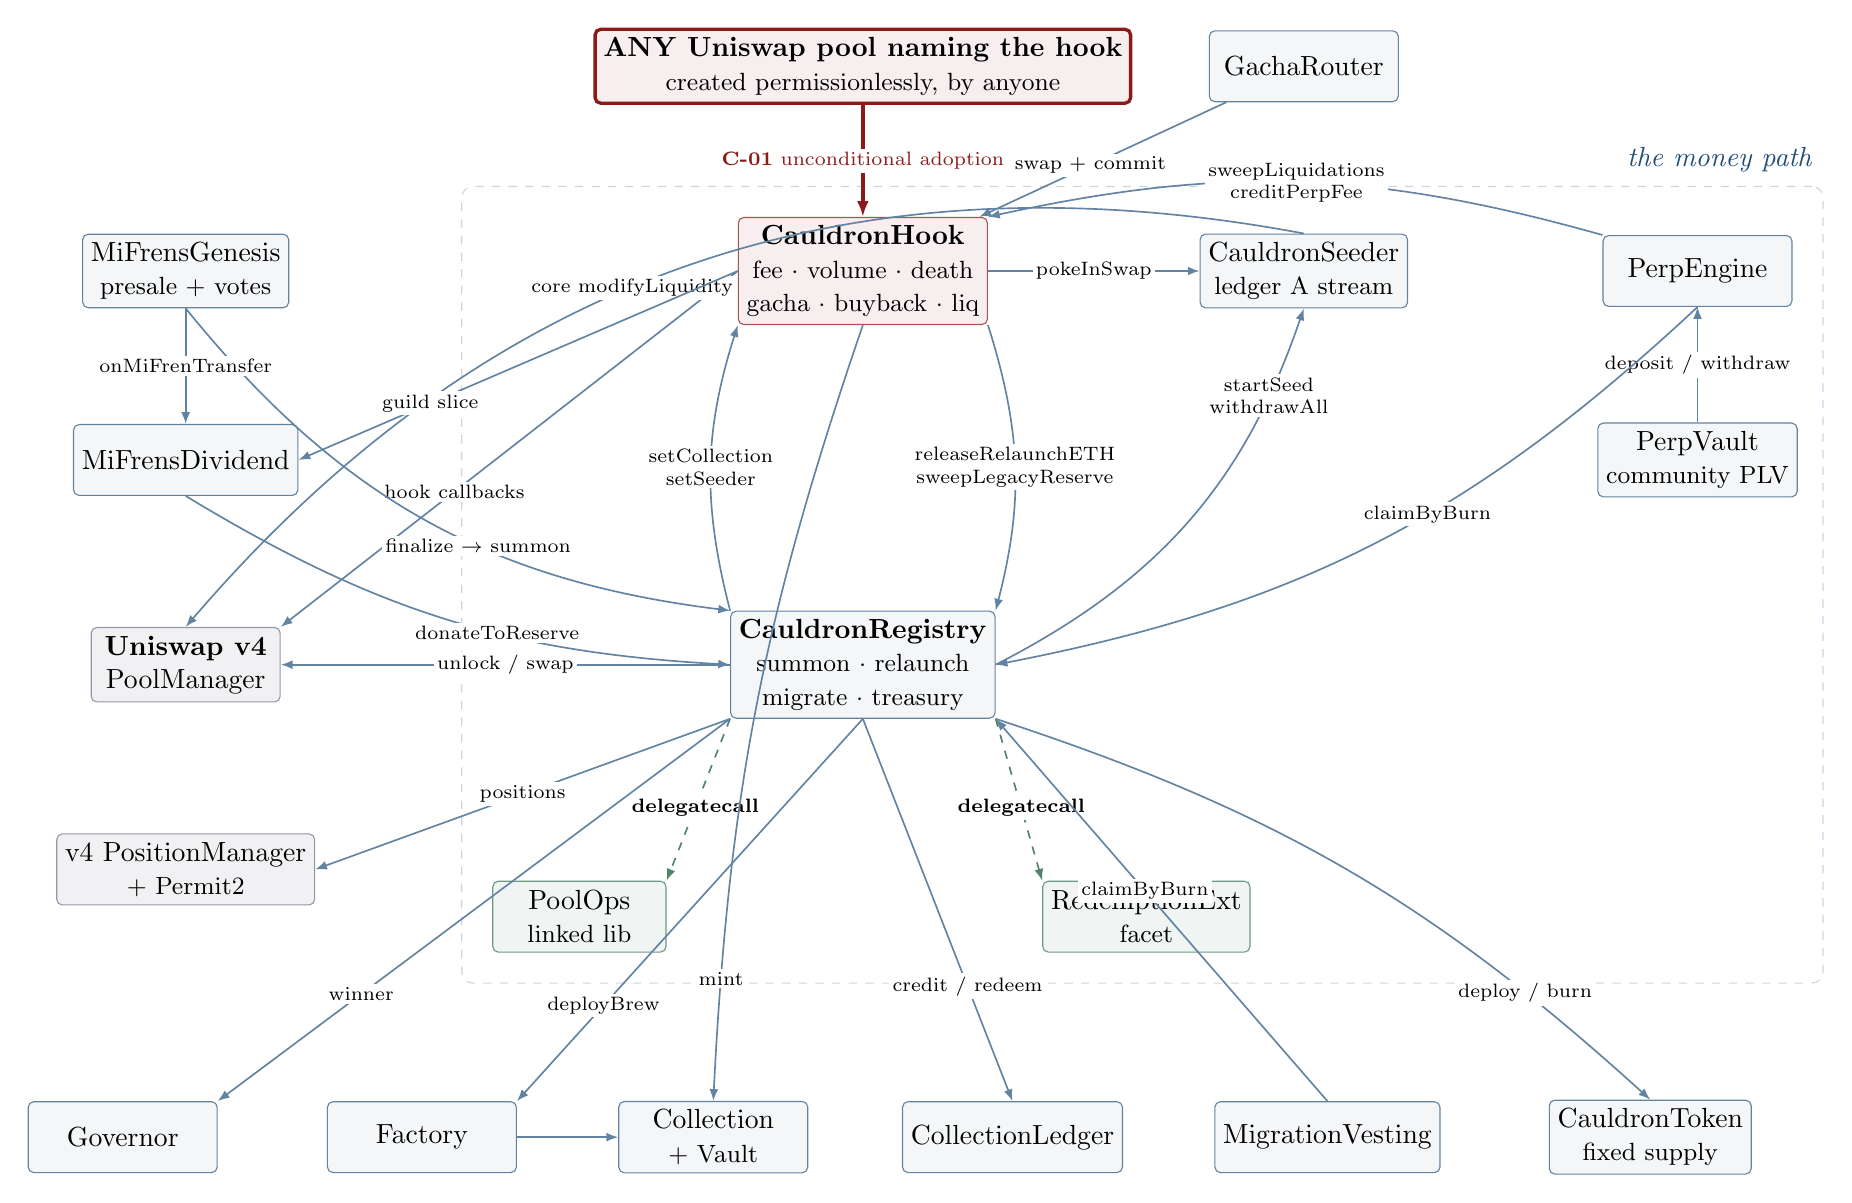
\begin{tikzpicture}[
  font=\normalsize,
  box/.style={draw=cauldronblue!70,fill=cauldronblue!5,rounded corners=2pt,
              minimum height=9mm,minimum width=24mm,inner sep=3pt,align=center},
  ext/.style={draw=sevinfo!60,fill=sevinfo!8,rounded corners=2pt,
              minimum height=9mm,minimum width=24mm,inner sep=3pt,align=center},
  lib/.style={draw=sevlow!70,fill=sevlow!7,rounded corners=2pt,
              minimum height=9mm,minimum width=22mm,inner sep=3pt,align=center},
  hot/.style={draw=sevcrit!75,fill=sevcrit!7,rounded corners=2pt,
              minimum height=9mm,minimum width=26mm,inner sep=3pt,align=center},
  flow/.style={-{Latex[length=1.5mm]},draw=cauldronblue!70,semithick},
  dele/.style={-{Latex[length=1.5mm]},draw=sevlow!85,semithick,dashed},
  danger/.style={-{Latex[length=2mm]},draw=sevcrit,very thick},
  lbl/.style={font=\scriptsize,inner sep=1.2pt,fill=white,align=center}
]

%------ row 0 : the unguarded boundary --------------------------------------
\node[hot,draw=sevcrit,very thick,minimum width=54mm] (any) at (0,5.6)
      {\textbf{ANY Uniswap pool naming the hook}\\{\small created permissionlessly, by anyone}};

%------ row 1 : genesis / dividend ------------------------------------------
\node[box] (mif)  at (-8.6,3.0) {MiFrensGenesis\\{\small presale + votes}};
\node[box] (div)  at (-8.6,0.6) {MiFrensDividend};

%------ row 2 : the hook + its satellites -----------------------------------
\node[hot] (hook) at ( 0,3.0) {\textbf{CauldronHook}\\{\small fee $\cdot$ volume $\cdot$ death}\\{\small gacha $\cdot$ buyback $\cdot$ liq}};
\node[box] (seed) at ( 5.6,3.0) {CauldronSeeder\\{\small ledger A stream}};
\node[box] (perp) at (10.6,3.0) {PerpEngine};
\node[box] (pvlt) at (10.6,0.6) {PerpVault\\{\small community PLV}};
\node[box] (gach) at ( 5.6,5.6) {GachaRouter};

%------ row 3 : the venue + the orchestrator --------------------------------
\node[ext] (pm)   at (-8.6,-2.0) {\textbf{Uniswap v4}\\PoolManager};
\node[box] (reg)  at ( 0,-2.0) {\textbf{CauldronRegistry}\\{\small summon $\cdot$ relaunch}\\{\small migrate $\cdot$ treasury}};
\node[ext] (posm) at (-8.6,-4.6) {v4 PositionManager\\{\small + Permit2}};

%------ row 4 : delegatecall pair -------------------------------------------
\node[lib] (ops)  at (-3.6,-5.2) {PoolOps\\{\small linked lib}};
\node[lib] (ext2) at ( 3.6,-5.2) {RedemptionExt\\{\small facet}};

%------ row 5 : the periphery -----------------------------------------------
\node[box] (gov)  at (-9.4,-8.0) {Governor};
\node[box] (fac)  at (-5.6,-8.0) {Factory};
\node[box] (col)  at (-1.9,-8.0) {Collection\\{\small + Vault}};
\node[box] (led)  at ( 1.9,-8.0) {CollectionLedger};
\node[box] (vest) at ( 5.9,-8.0) {MigrationVesting};
\node[box] (tok)  at (10.0,-8.0) {CauldronToken\\{\small fixed supply}};

%------ the finding -----------------------------------------------------------
\draw[danger] (any) -- node[lbl,text=sevcrit]{\textbf{C-01} unconditional adoption} (hook);

%------ hook <-> venue / registry --------------------------------------------
\draw[flow] (hook.west)  -- node[lbl,pos=0.62]{hook callbacks} (pm.north east);
\draw[flow] (reg.west)   -- node[lbl,pos=0.5]{unlock / swap} (pm.east);
\draw[flow] (reg.south west) -- node[lbl,pos=0.5]{positions} (posm.east);
\draw[flow] (reg.north west) to[bend left=16] node[lbl,pos=0.5]{setCollection\\setSeeder} (hook.south west);
\draw[flow] (hook.south east) to[bend left=16] node[lbl,pos=0.5]{releaseRelaunchETH\\sweepLegacyReserve} (reg.north east);

%------ delegatecall pair ------------------------------------------------------
\draw[dele] (reg.south west) -- node[lbl,pos=0.55]{\textbf{delegatecall}} (ops.north east);
\draw[dele] (reg.south east) -- node[lbl,pos=0.55]{\textbf{delegatecall}} (ext2.north west);

%------ seeder ---------------------------------------------------------------
\draw[flow] (hook) -- node[lbl]{pokeInSwap} (seed);
\draw[flow] (reg.east) to[bend right=22] node[lbl,pos=0.82]{startSeed\\withdrawAll} (seed.south);
\draw[flow] (seed.north) to[bend right=30] node[lbl,pos=0.55]{core modifyLiquidity} (pm.north);

%------ perps ----------------------------------------------------------------
\draw[flow] (perp.north west) to[bend right=14] node[lbl,pos=0.5]{sweepLiquidations\\creditPerpFee} (hook.north east);
\draw[flow] (pvlt) -- node[lbl]{deposit / withdraw} (perp);
\draw[flow] (perp.south) to[bend left=16] node[lbl,pos=0.42]{claimByBurn} (reg.east);

%------ lifecycle -------------------------------------------------------------
\draw[flow] (reg.south west) -- node[lbl,pos=0.72]{winner} (gov.north east);
\draw[flow] (reg.south) -- node[lbl,pos=0.75]{deployBrew} (fac.north east);
\draw[flow] (fac) -- (col);
\draw[flow] (hook.south) to[bend right=8] node[lbl,pos=0.86]{mint} (col.north);
\draw[flow] (reg.south) -- node[lbl,pos=0.7]{credit / redeem} (led.north);
\draw[flow] (vest.north) -- node[lbl,pos=0.55]{claimByBurn} (reg.south east);
\draw[flow] (reg.south east) to[bend left=12] node[lbl,pos=0.8]{deploy / burn} (tok.north);

%------ genesis + play --------------------------------------------------------
\draw[flow] (mif.south) to[bend right=22] node[lbl,pos=0.6]{finalize $\to$ summon} (reg.north west);
\draw[flow] (hook.west) -- node[lbl,pos=0.7]{guild slice} (div.east);
\draw[flow] (mif) -- node[lbl]{onMiFrenTransfer} (div);
\draw[flow] (div.south) to[bend right=14] node[lbl,pos=0.6]{donateToReserve} (reg.west);
\draw[flow] (gach) -- node[lbl,pos=0.55]{swap + commit} (hook);

\begin{scope}[on background layer]
\node[draw=rulegray,dashed,rounded corners,fit=(hook)(reg)(ops)(ext2)(seed)(perp),
      inner sep=11pt] (money) {};
\node[font=\normalsize,text=cauldronblue,above left=0.5mm and 0mm of money.north east]
      {\textit{the money path}};
\end{scope}
\end{tikzpicture}}
\end{center}

\noindent
Solid arrows are ordinary external calls; dashed green arrows are
\code{delegatecall} (the callee runs in the registry's storage and custody); the
red arrow is the unguarded boundary that produces both Critical findings.

\subsection{The token lifecycle}

\begin{center}
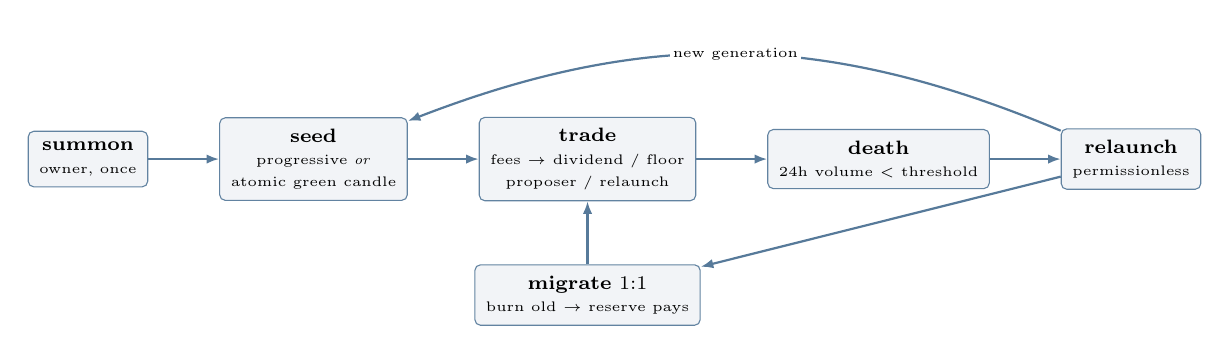
\begin{tikzpicture}[font=\scriptsize,node distance=4mm,
  st/.style={draw=cauldronblue!70,fill=cauldronblue!6,rounded corners=2pt,minimum height=7mm,inner sep=4pt,align=center},
  ar/.style={-{Latex[length=1.6mm]},thick,draw=cauldronblue!75}]
\node[st] (a) {\textbf{summon}\\{\tiny owner, once}};
\node[st,right=9mm of a] (b) {\textbf{seed}\\{\tiny progressive \emph{or}}\\{\tiny atomic green candle}};
\node[st,right=9mm of b] (c) {\textbf{trade}\\{\tiny fees $\to$ dividend / floor}\\{\tiny proposer / relaunch}};
\node[st,right=9mm of c] (d) {\textbf{death}\\{\tiny 24h volume $<$ threshold}};
\node[st,right=9mm of d] (e) {\textbf{relaunch}\\{\tiny permissionless}};
\node[st,below=8mm of c] (f) {\textbf{migrate} $1{:}1$\\{\tiny burn old $\to$ reserve pays}};
\draw[ar] (a)--(b); \draw[ar] (b)--(c); \draw[ar] (c)--(d); \draw[ar] (d)--(e);
\draw[ar] (e) to[bend right=22] node[font=\tiny,fill=white,inner sep=1pt,pos=0.5]{new generation} (b);
\draw[ar] (e) -- (f);
\draw[ar] (f) -- (c);
\end{tikzpicture}
\end{center}

\subsection{Two ledgers, one reserve}

The clearest idea in the design is the separation between \emph{ledger A} (the
active, tradeable tranche) and \emph{ledger B} (the reserve). Only ledger A is
ever handed to the seeder; ledger B is placed by the registry directly and its
position NFT never leaves the registry's custody. This makes ``the seeder can
never touch the redemption reserve'' a structural property rather than a
behavioural one, and I encoded it as invariant~\textbf{I-4}
(\S\ref{sec:invariants}), which holds under fuzzing.

The orientation of ledger B is subtle enough to be worth restating, because
getting it backwards would silently destroy the protocol's entire backing. ETH
is \code{currency0} and the brew token is \code{currency1}, so the pool price is
\emph{tokens per ETH}. When the token appreciates, tokens-per-ETH \emph{falls},
so the tick \emph{falls}. A position is pure \code{token1} only when the current
price is \emph{above} its range. Therefore the reserve must sit \emph{below} the
launch tick --- and \code{ReserveLib.reserveTicks}
(\code{ReserveLib.sol:49}) does exactly that. I verified this under fuzzing
across the whole reachable tick domain
(\code{testFuzz\_ReserveSitsBelowLaunchTick}).

%==============================================================================
\section{The delegatecall facet}
\label{sec:facet}

\code{CauldronRegistry} exceeds EIP-170 on its own, so four OG-redemption
entrypoints were moved into \code{RedemptionExt} and are reached through a
raw-assembly \code{delegatecall} forwarder (\code{CauldronRegistry.sol:965}).
This is the highest-risk structural pattern in the codebase --- a delegatecall
target has full code-execution power over the caller's storage and custody ---
so it deserves its own verification, and it passes.

\begin{enumerate}
\item \textbf{Layout equality.} Both contracts derive from
\code{CauldronBase} and neither adds state, so the layouts are identical
\emph{by construction}. I confirmed it mechanically: both report 52 slots with
identical labels, slots and offsets. The only differences are solc AST node
identifiers embedded in type strings (e.g.\ \code{t\_contract(IPoolManager)12919}
vs \code{...10372}), which are compilation artefacts, not layout.

\item \textbf{The immutable trap is correctly avoided.}
\code{poolManager}, \code{positionManager} and \code{hook} were immutables in
the monolith. Immutables live in the \emph{executing} contract's code, so under
delegatecall the facet would read them as zero and every redemption would call
into \code{address(0)}. \code{CauldronBase.sol:259--261} correctly promotes all
three to storage. This is a real trap that the code sidesteps deliberately.

\item \textbf{The reentrancy-guard interaction is correct and non-obvious.}
The facet's functions carry \code{nonReentrant}, which under delegatecall
operates on the \emph{registry's} guard slot (OZ~5.6 uses a fixed ERC-7201
namespace, not a layout-dependent slot). The forwarders therefore must
\emph{not} also be \code{nonReentrant} --- and they are not
(\code{CauldronRegistry.sol:937--957}). Adding a guard there would double-lock
and revert every redemption. The comment at line 929 shows this was understood.

\item \textbf{A direct call to the facet is inert.} Its own storage has
\code{summoned == false}, so every entrypoint reverts \code{NotSummoned} before
touching value, and it custodies nothing.

\item \textbf{The zero-target check is right for the right reason.}
\code{\_forwardToExt} rejects \code{address(0)}, and \code{setRedemptionExt}
rejects code-less targets (\code{CauldronRegistry.sol:148}). A delegatecall to
an empty account returns \emph{success with no returndata}, which would make
every redemption a silent no-op returning zero rather than a revert. Catching
this is a genuinely sharp piece of defensive engineering.
\end{enumerate}

\noindent All five properties are encoded in
\code{test/invariants/FacetLayoutInvariant.t.sol}, including a fuzz test that
runs the facet's compiled code against a third contract's storage image and
checks it reads the right slots.

%==============================================================================
\section{Invariants}
\label{sec:invariants}

Below are the protocol's advertised guarantees, restated formally, with a
verdict for each. ``Holds'' means I could neither construct a counterexample by
hand nor find one under fuzzing; ``Conditional'' means it holds only under a
stated assumption; ``Breaks'' means I have a passing exploit.

\subsubsection*{I-1 --- Supply is fixed and never inflates}
\[
\forall g:\; \mathrm{totalSupply}(T_g) \le \textsc{total\_supply}
\quad\wedge\quad
\mathrm{totalSupply}(T_{\mathrm{current}}) = \textsc{total\_supply}
\]
\textbf{Verdict: holds.} \code{CauldronToken} has no \code{mint()}; the entire
supply is minted once in the constructor to the registry
(\code{CauldronToken.sol:46}) and \code{burn} is registry-gated and
monotonically decreasing. A retired generation's supply can only shrink, via
relaunch's LP burn (\code{CauldronRegistry.sol:596}), migration
(\code{PoolOps.migrateOne}) and the legacy flush. Encoded as
\code{invariant\_supplyIsFixedAndNeverInflates}.

\subsubsection*{I-2 --- Migration is $1{:}1$}
\[
\Delta\,\mathrm{received}_{\mathrm{new}} = \Delta\,\mathrm{burned}_{\mathrm{old}}
\]
\textbf{Verdict: conditional --- and the failure mode is unsafe
(\textbf{H-03}).} The \emph{safe} half holds unconditionally: a claimer can
never receive more than they burned. The other half does not. \code{claimByBurn}
burns \code{amount} and then takes whatever \code{claimFromReserve} yields,
without comparing them. While the reserve is sufficient the gap is
liquidity-quantization dust --- I measured \textbf{276 wei} on a
$2.8\times10^{26}$ claim --- but when the reserve is short the same missing
check silently destroys the difference. Encoded as two invariants
(\code{invariant\_migrationNeverOverDelivers}, which is the hard safety
property, and \code{invariant\_migrationShortfallIsDustOnly}, which bounds the
benign case) plus an explicit regression test pinning the deviation.

\subsubsection*{I-3 --- The reserve always backs its claims}
\[
\mathrm{reserveTokens}(g) \;\ge\;
\underbrace{\textsc{genesisReserveOutstanding}}_{\text{OG floor}}
\;+\;
\underbrace{\textstyle\sum_{k}\textsc{entitledTokens}(k)}_{\text{legacy floors}}
\]
\textbf{Verdict: holds, by careful construction.} The design decision that makes
this work is that \code{materializeLegacyReserve} deposits the bought tokens
\emph{and} credits the ledger in one call
(\code{RedemptionExt.sol:118}), so a credit can never out-run the backing. The
ledger side is separately proved: \code{invariant\_entitlementNeverExceedsCredited}
shows a generation's entitlement never exceeds what was credited to it, and
\code{invariant\_totalEntitledEqualsSum} shows the global sum never drifts.
The system-level version is \code{invariant\_reserveBacksItsClaims}, which reads
the live position's token amount from the fork.

\subsubsection*{I-4 --- The seeder only ever touches ledger A}
\textbf{Verdict: holds, structurally.} The reserve position NFT is minted to and
owned by the registry (\code{PoolOps.\_seedReserve}); the seeder is funded by a
scoped \code{approve} for exactly \code{activeTokens} and pulls only that
(\code{PoolOps.sol:270--277}). Encoded as
\code{invariant\_seederNeverOwnsTheReserve}, which additionally checks that no
tracked seeder range ever coincides with the reserve band.

\subsubsection*{I-5 --- Registry and facet storage layouts are byte-identical}
\textbf{Verdict: holds.} See \S\ref{sec:facet}.

\subsubsection*{I-6 --- Hook ETH accounting is backed by real ETH}
\[
\mathrm{balance}(\textsc{hook}) \;\ge\; \textsc{relaunchETH} + \textsc{legacyBuffer}
\]
\textbf{Verdict: BREAKS (\textbf{C-01}).} For pools the protocol created this
holds --- and the invariant passes under fuzzing against a legitimate pool. But
a swap in \emph{any} pool naming the hook can inflate \code{relaunchETH} with
units of a worthless token, so the accounting exceeds the balance and
\code{releaseRelaunchETH} reverts forever. The invariant is written to be
sensitive to this so a future fix can be validated against it.

\subsubsection*{I-7 --- Perp engine solvency}
\[
\mathrm{balance}_{\mathrm{ETH}}(\textsc{engine}) \ge \textsc{plv} + \textsc{insuranceEth} + \textsc{tokYieldEth}
\quad\wedge\quad
\mathrm{balance}_{\mathrm{token}} \ge \textsc{plvToken}
\]
\textbf{Verdict: holds.} The subtle part is bad debt, and both directions are
handled correctly and \emph{differently}: on the long path \code{plv} has
already booked the reduced repayment so insurance \emph{replenishes} it
(\code{\_replenishPlv}), while on the short path the buy-back overspent raw ETH
that was never booked, so the loss must be \emph{absorbed}
(\code{\_absorbPlvLoss}), saturating at zero. Getting these backwards would be a
silent insolvency; the code gets them right. Encoded as
\code{invariant\_perpEngineIsSolvent}.

\subsubsection*{I-8 --- PLV principal is protected against governance}
\textbf{Verdict: holds for the vault pointer; \emph{fails} for insurance.}
\code{setVault} cannot be re-pointed while any depositor funds are staked
(\code{PerpEngine.sol:1188}) --- a genuinely good guard that blocks the obvious
owner-drain path. But \code{skimInsurance} only protects \code{insuranceFloor},
which defaults to \code{0}, so the owner can withdraw the entire bad-debt buffer
that is actively backing open positions (\textbf{M-05}).

\subsubsection*{I-9 --- The exit guarantee}
\[
\text{redeem blocked} \iff \textsc{redemptionPaused} \wedge (\textsc{emergencyReadyAt} = 0)
\]
\textbf{Verdict: holds.} The instant a custody action is armed, the exit is
forced open, so holders can always leave at floor \emph{before} anything moves
(\code{CauldronBase.sol:292}). This is a strong design choice and it is
implemented exactly as documented. Fuzzed in
\code{testFuzz\_ExitGuarantee}.

\subsubsection*{I-10 --- The progressive stream cannot be accelerated}
\textbf{Verdict: holds mathematically; \emph{fails operationally}
(\textbf{H-02}).} \code{SeedLib.deployedTargetWad} is a pure function of elapsed
time, monotone and capped at $10^{18}$ --- proved under fuzzing
(\code{testFuzz\_ScheduleIsMonotoneAndCapped}) --- so no caller can over-deploy
or block the stream. But the seeder never resets \code{complete} between
campaigns, so from generation~2 onward the stream never starts at all.

\subsubsection*{I-11 --- Relaunch is conserved: no dilution}
\textbf{Verdict: holds.} Relaunch mints nothing to the caller and burns
everything it recovers from the dead LP (\code{CauldronRegistry.sol:596}). The
new active tranche mirrors the rescued tokens minus outstanding genesis and
legacy claims, and the reserve is \code{TOTAL\_SUPPLY - newActive} --- so the
split is sized to actual obligations rather than a fixed fraction. The degenerate
guards at lines 673--676 prevent a zero-seed.

%==============================================================================
\section{Findings}

Findings are ordered by severity. Each states its location, the mechanism, a
concrete exploit path, the impact, and a specific code-level fix.

%------------------------------------------------------------------------------
\finding{C-01a}{Unbounded hook adoption mints phantom \texttt{relaunchETH}, permanently bricking \texttt{relaunch()}}{Critical}{Confirmed}{sevcrit}

\loc{CauldronHook.sol:473 \texttt{\_afterInitialize} \textbullet\ :943 \texttt{\_takeEthFee} \textbullet\ :1077 \texttt{releaseRelaunchETH}}

\textbf{Mechanism.} Uniswap~v4 lets anyone initialize a pool with any hook
address whose permission bits match. \code{CauldronHook} adopts every such pool
without question:

\begin{lstlisting}[firstnumber=473]
function _afterInitialize(address, PoolKey calldata key, uint160, int24)
    internal override returns (bytes4)
{
    PoolId id = key.toId();
    trackedPools[id] = true;          // <-- no allow-list, no currency check
    _lastUpdateBlock[id] = block.number;
    poolInitBlock[id] = block.number;
    emit PoolTracked(id);
    return BaseHook.afterInitialize.selector;
}
\end{lstlisting}

The hook's entire fee engine then assumes what is true only for pools the
protocol created: that \code{currency0} is native ETH. \code{\_beforeSwap}
checks this explicitly (line 760, \code{Currency.unwrap(key.currency0) ==
address(0)}) --- but \code{\_afterSwap} does not. It decides the sell leg
applies purely from swap direction and exactness:

\begin{lstlisting}[firstnumber=635]
bool exactInput = params.amountSpecified < 0;
bool unspecifiedIsEth = exactInput ? (!params.zeroForOne) : (params.zeroForOne);
if (!unspecifiedIsEth) return (BaseHook.afterSwap.selector, 0);
...
uint256 fee = _takeEthFee(key, sender, ethAmount, false);
\end{lstlisting}

\noindent and \code{\_takeEthFee} takes \code{key.currency0} --- \emph{whatever
that token is} --- then credits the proceeds to ETH-denominated counters:

\begin{lstlisting}[firstnumber=961]
poolManager.take(key.currency0, address(this), total);   // an arbitrary ERC20
...
else _routeEthFee(baseFee);                              // -> relaunchETH += ...
\end{lstlisting}

\textbf{Exploit path.} One transaction, no capital at risk:
\begin{enumerate}
\item Deploy two worthless ERC-20s, \code{A} and \code{B}.
\item \code{poolManager.initialize} the pool \code{(A, B)} naming the Cauldron
hook. Both are ERC-20s, so \emph{neither} leg is ETH.
\item Add your own liquidity, then swap \code{B}$\to$\code{A} exact-input. Now
\code{zeroForOne == false} and \code{exactInput == true}, so
\code{unspecifiedIsEth} is \code{true} and the hook charges its ``ETH'' fee ---
in units of \code{A}.
\item \code{relaunchETH} is now a large number backed by nothing.
\end{enumerate}

\noindent Measured on a Sepolia fork
(\code{test/audit/AuditPoC.t.sol::test\_PoC\_PhantomRelaunchEth\_BricksRelaunch}):

\begin{center}\small
\begin{tabular}{@{}lr@{}}
\toprule
\code{relaunchETH} after one attacker swap & $989{,}374{,}614{,}163{,}774{,}780{,}306$ (\textasciitilde{}0.99 ``ETH'') \\
Hook's actual ETH balance & $0$ \\
\code{releaseRelaunchETH()} & \textbf{reverts} \code{"ETH transfer failed"} \\
\bottomrule
\end{tabular}
\end{center}

\textbf{Impact.} \code{CauldronRegistry.relaunch()} calls
\code{releaseRelaunchETH()} whenever \code{relaunchETH > 0}
(\code{CauldronRegistry.sol:615}), and that call is \emph{not} wrapped in
try/catch --- \code{require(ok, "ETH transfer failed")} propagates. So the
protocol's central, permissionless, self-funding function reverts forever. There
is no reset path: \code{relaunchETH} is only ever zeroed inside the function
that now always reverts. Because \code{emergencySweep} moves ETH but not the
counter, even the break-glass admin cannot clear it. The eternal machine stops
being eternal, and every generation's holders lose the migration path that
depends on relaunch. The attack costs one pool creation plus gas and can be
repeated after any hypothetical manual reset.

\textbf{Fix.} Restrict adoption to pools the protocol created, and defend in
depth on the fee path:

\begin{lstlisting}[numbers=none]
// 1. Only the registry's own pools are ever tracked.
function _afterInitialize(address sender, PoolKey calldata key, uint160, int24)
    internal override returns (bytes4)
{
    if (sender != registry) return BaseHook.afterInitialize.selector; // ignore
    if (Currency.unwrap(key.currency0) != address(0)) revert ZeroAddress();
    PoolId id = key.toId();
    trackedPools[id] = true;
    _lastUpdateBlock[id] = block.number;
    poolInitBlock[id] = block.number;
    emit PoolTracked(id);
    return BaseHook.afterInitialize.selector;
}

// 2. Belt and braces: never charge the ETH fee on a non-ETH pool.
//    In _afterSwap, before the fee block:
if (Currency.unwrap(key.currency0) != address(0) || !trackedPools[id]) {
    return (BaseHook.afterSwap.selector, 0);
}
\end{lstlisting}

\noindent Note that returning the selector without tracking (rather than
reverting) is deliberate: reverting in \code{afterInitialize} would let anyone
grief \emph{pool creation}, whereas ignoring the pool simply declines to serve
it. Because \code{registry} is set once and the registry initializes every
legitimate pool through \code{PoolOps}, the \code{sender} check is exact.

%------------------------------------------------------------------------------
\finding{C-01b}{The legacy buyback spends the hook's ETH inside an attacker-chosen pool}{Critical}{Confirmed}{sevcrit}

\loc{CauldronHook.sol:662 \texttt{\_maybeLegacyBuyback} \textbullet\ :694 \texttt{legacyBuyStep}}

\textbf{Mechanism.} The same missing boundary, but this one moves real money.
When the buyback buffer is full, \code{\_afterSwap} fires a self-call at the
\emph{top} of the function --- before any pool validation --- passing the
\code{PoolKey} of \emph{the swap currently executing}:

\begin{lstlisting}[firstnumber=662]
function _maybeLegacyBuyback(PoolKey calldata key) private {
    if (legacyRegistry == address(0) || legacyBuffer < legacyThreshold) return;
    uint256 gl = gasleft();
    if (gl > LEGACY_GAS_MIN) {
        address(this).call{gas: gl - LEGACY_GAS_RESERVE}(
            abi.encodeWithSelector(this.legacyBuyStep.selector, key)   // attacker's key
        );
    }
}
\end{lstlisting}

\noindent \code{legacyBuyStep} then spends the \emph{entire} buffer buying
\code{key.currency1} --- whatever the attacker chose --- and pays for it with
the hook's real ETH:

\begin{lstlisting}[firstnumber=700]
_inSelfBuy = true;
BalanceDelta d = poolManager.swap(key, SwapParams({zeroForOne: true,
    amountSpecified: -int256(amt), sqrtPriceLimitX96: MIN_SQRT_LIMIT}), "");
_inSelfBuy = false;
poolManager.settle{value: amt}();               // <-- the hook's ETH leaves
\end{lstlisting}

\textbf{Exploit path.}
\begin{enumerate}
\item Deploy a worthless ERC-20 \code{E} and initialize \code{(ETH, E)} naming
the hook, priced so that ETH buys an enormous quantity of \code{E}.
\item Seed it with your own liquidity.
\item Swap a trivial amount (0.001~ETH). In \code{afterSwap}, the hook sees a
full buffer and buys \code{E} with all of it --- inside \emph{your} pool.
\item Withdraw your liquidity. The hook's ETH is now yours; the hook holds
worthless \code{E}.
\end{enumerate}

\noindent Measured on a Sepolia fork
(\code{test/audit/AuditPoC.t.sol::test\_PoC\_LegacyBufferTheft}):

\begin{center}\small
\begin{tabular}{@{}lrr@{}}
\toprule
& \textbf{before} & \textbf{after} \\
\midrule
Hook ETH balance    & 5.000 ETH & \textbf{0.000 ETH} \\
Hook \code{legacyBuffer} & 5.000 ETH & 0 \\
Attacker ETH        & 495.000 ETH & \textbf{500.000 ETH} \\
Hook \code{EVIL} received & --- & 13.26 (worthless) \\
\bottomrule
\end{tabular}
\end{center}

\textbf{Impact.} Direct, repeatable theft of every ETH the hook accumulates in
its buyback buffer, with a probe swap of arbitrarily small size. Under the
shipped configuration (\code{DeployLaunchpad.s.sol}: \code{LEGACY\_BPS=4000},
\code{LEGACY\_THRESHOLD=0.02 ether}) the buffer is continuously refilled from
40\,\% of the post-guild fee, so this is a standing tap on protocol revenue that
would otherwise back the live collection's NFT floor. The attacker also
poisons \code{legacyOwedToReserve} with a claim on tokens the hook does not hold
in the live token, though \code{sweepLegacyReserve} caps at the real balance so
that part is contained.

\textbf{Fix.} Never spend on a key the caller supplied. Drive the buyback from
the protocol's own live pool key:

\begin{lstlisting}[numbers=none]
// Store the live key when the registry wires the generation.
PoolKey private _liveKey;
function setLiveKey(PoolKey calldata k) external {
    if (msg.sender != registry) revert OnlyRegistry();
    _liveKey = k;
}

function _maybeLegacyBuyback(PoolKey calldata key) private {
    if (legacyRegistry == address(0) || legacyBuffer < legacyThreshold) return;
    // ONLY ever buy in the protocol's own pool.
    if (PoolId.unwrap(key.toId()) != PoolId.unwrap(_liveKey.toId())) return;
    ...
        abi.encodeWithSelector(this.legacyBuyStep.selector, _liveKey)
}
\end{lstlisting}

\noindent The \code{trackedPools} fix in C-01a is necessary but \emph{not}
sufficient here: an attacker pool would still be tracked if the allow-list were
keyed on tracking alone. Pin the key.

%------------------------------------------------------------------------------
\finding{C-02}{A winning proposal with an out-of-range \texttt{nftSupply} freezes the protocol permanently}{Critical}{Confirmed}{sevcrit}

\loc{CauldronGovernor.sol:123 \texttt{propose} \textbullet\ CauldronRegistry.sol:641,745 \textbullet\ CauldronCollection.sol:126}

\textbf{Mechanism.} \code{propose()} validates the name, symbol and metadata
source, but places \emph{no bound} on \code{nftSupply}:

\begin{lstlisting}[firstnumber=137]
if (bytes(name).length == 0 || bytes(symbol).length == 0) revert EmptyField();
if (mode == MetadataMode.BaseURI) {
    if (bytes(baseURI).length == 0) revert EmptyField();
} else {
    if (renderer == address(0) || renderer.code.length == 0) revert BadRenderer();
}
// nftSupply and volumePerNFT: unvalidated
\end{lstlisting}

\noindent \code{relaunch()} adopts it verbatim (\code{if (spec.nftSupply > 0)
nftSupply = spec.nftSupply;}, line 641) and passes it to the factory, whose
collection constructor enforces a hard bound so art ids can never collide with
Liquidatoor badge ids:

\begin{lstlisting}[firstnumber=126]
if (minter_ == address(0) || maxSupply_ == 0 || maxSupply_ >= LIQUIDATOR_ID_BASE)
    revert BadConfig();          // LIQUIDATOR_ID_BASE == 1_000_000
\end{lstlisting}

\noindent The bound is correct. The problem is \emph{where} it fires. The revert
propagates out of \code{relaunch()}, and because \code{governor.markConsumed(winId)}
executed earlier \emph{in the same transaction} (line 643), it is rolled back
too. The poisoned proposal is never retired, so it wins again on the next
attempt, forever.

\textbf{Exploit path.} Any MiFren holder proposes a brew with
\code{nftSupply = 1\_000\_000} and accumulates enough votes to lead. It need not
even be malicious --- a proposer who wants a one-million-piece collection
triggers it by accident. When the generation dies, every \code{relaunch()} call
reverts.

\noindent Verified on a Sepolia fork
(\code{test/audit/AuditPoC4.t.sol}): \code{relaunch()} reverts
\code{CauldronCollection.BadConfig}, \code{markConsumed} is rolled back
(\code{gov.consumed() == false}), the generation stays at 1, and a second
attempt reverts identically.

\textbf{Impact.} Permanent, unrecoverable freeze of the eternal machine. No
relaunch means: no new generation, no migration target for existing holders, no
perp \code{syncGeneration}, and the dead pool's LP stays locked in a
zero-volume pool. \emph{The only escape is \code{setGovernor}, which is
\code{onlyOwner}} --- and \code{DeployLaunchpad.s.sol:248} transfers registry
ownership to the \code{MiFrensGenesis} presale contract, which exposes no call
that would forward to it. So on the shipped deployment there is no recovery
short of \code{migrateToSuccessor} --- a full V2 migration behind the emergency
timelock. My PoC demonstrates recovery via \code{setGovernor} only to prove that
is the sole exit.

\textbf{Fix.} Validate at the boundary, and make relaunch resilient to a bad
winner:

\begin{lstlisting}[numbers=none]
// 1. CauldronGovernor.propose -- reject what can never be launched.
uint256 constant MAX_NFT_SUPPLY = 100_000;   // << LIQUIDATOR_ID_BASE
if (nftSupply > MAX_NFT_SUPPLY) revert EmptyField();

// 2. CauldronRegistry.relaunch -- clamp defensively as well, so a governor
//    swapped in later cannot re-introduce the freeze.
if (spec.nftSupply > 0) {
    nftSupply = spec.nftSupply > MAX_NFT_SUPPLY ? MAX_NFT_SUPPLY : spec.nftSupply;
}
\end{lstlisting}

\noindent The same reasoning applies to every other field of \code{BrewSpec}
that reaches a constructor. \code{renderer} is already checked for code size at
proposal time, but note it is checked \emph{again} in the collection constructor
--- a renderer that self-destructs between proposal and relaunch would reproduce
this exact freeze. Clamping in \code{relaunch} covers both.

%------------------------------------------------------------------------------
\finding{H-01}{The collection's \texttt{deployer} is the factory, so the entire legacy-floor recycle path is unreachable}{High}{Confirmed}{sevhigh}

\loc{CauldronFactory.sol:37 \textbullet\ CauldronCollection.sol:134,296 \textbullet\ PoolOps.sol:716,740}

\textbf{Mechanism.} \code{CauldronCollection} records
\code{deployer = msg.sender} in its constructor (line 134). Because collections
are created \emph{by the factory} (\code{new CauldronCollection(...)} at
\code{CauldronFactory.sol:37}), \code{deployer} is the \textbf{factory address},
not the registry. But the custody entrypoint the legacy-floor design depends on
is gated on \code{deployer}:

\begin{lstlisting}[firstnumber=296]
function custodyTransfer(address from, address to, uint256 tokenId) external {
    if (msg.sender != deployer) revert OnlyVault();   // deployer == the FACTORY
    _transfer(from, to, tokenId);
}
\end{lstlisting}

\noindent while the caller is always the registry:

\begin{lstlisting}[firstnumber=712]
if (ICollectionOps(collection).ownerOf(tokenId) != caller) revert("not owner");
uint256 payout = ILedgerOps(ledger).redeem(gen, mintedNow);
ICollectionOps(collection).custodyTransfer(caller, address(this), tokenId); // reverts
\end{lstlisting}

\noindent The factory exposes only \code{deployBrew} and \code{deployVault} ---
there is no forwarding function --- so \emph{no address in the system} can pass
the gate.

\textbf{Impact.} Three separate consequences, all confirmed by test
(\code{test/audit/AuditPoC.t.sol::PoC\_CollectionCustodyLockout}):

\begin{enumerate}
\item \code{recycleCollectionNFT} and \code{buyCollectionNFT} always revert.
The collection legacy floor --- an entire subsystem with its own ledger,
crystallisation logic and $2\times$ buyback ratchet --- is dead code in
production. NFT holders can never redeem the floor their collection's own
volume paid for. Notably \code{ledger.redeem} is called \emph{before} the
reverting transfer, so the whole transaction rolls back and the ledger is not
corrupted --- the failure is clean, just total.
\item Every other \code{deployer}-gated admin function is permanently
unreachable: \code{setMetadata} (so a broken renderer can never be repointed,
defeating its stated purpose), \code{setTransferValidator} (so ERC-721C royalty
enforcement can never be switched on), \code{setLiquidatorURI}, and
\code{setRarityOdds}.
\item The genesis path is \emph{not} affected --- \code{MiFrensGenesis.custodyTransfer}
is correctly gated on \code{registry} (line 337), which is why OG redemption
works and the discrepancy is easy to miss.
\end{enumerate}

\textbf{Fix.} Pass the registry explicitly rather than inferring it from
\code{msg.sender}. The \code{Config} struct already carries it:

\begin{lstlisting}[numbers=none]
// CauldronCollection: take the controller as a constructor argument.
constructor(..., address registry_, ...) ERC721(name_, symbol_) {
    ...
    deployer = registry_;        // was: msg.sender (the factory)
}

// CauldronFactory.deployBrew: the vault wiring must then happen through a
// path the factory still controls, so do it before handing over -- or keep a
// separate `configurator` slot the factory holds and `deployer` for the registry:
//    address public immutable configurator; // = msg.sender (factory), setVault/setRoyalty
//    address public immutable deployer;     // = c.registry,  custodyTransfer/setMetadata
\end{lstlisting}

\noindent The two-slot variant is the safer refactor: the factory keeps exactly
the two rights it needs at deploy time (\code{setVault}, \code{setRoyalty}) and
the registry gets custody and the governed art/validator setters. Add a
regression test asserting \code{col.deployer() == address(registry)}.

%------------------------------------------------------------------------------
\finding{H-02}{\texttt{CauldronSeeder} never resets \texttt{complete}, so generation 2 onward never streams}{High}{Confirmed}{sevhigh}

\loc{CauldronSeeder.sol:125 \texttt{startSeed} \textbullet\ :182 \texttt{\_pendingStep} \textbullet\ :360 \texttt{withdrawAll}}

\textbf{Mechanism.} The seeder is explicitly designed to be persistent --- one
instance serves every generation (``\emph{Deployed once (pointed at this
registry) and reused every generation}'', \code{CauldronRegistry.sol:168}).
Teardown sets three flags:

\begin{lstlisting}[firstnumber=360]
function withdrawAll(address to) external onlyRegistry lock returns (...) {
    poolManager.unlock(abi.encode(ACT_WITHDRAW, to));
    ...
    delete ranges;
    seeding = false;
    complete = true;        // <-- sticky
}
\end{lstlisting}

\noindent but \code{startSeed} resets only \code{seeding}:

\begin{lstlisting}[firstnumber=145]
    seeding = true;
    // `complete`     : NOT reset
    // `_basePlaced`  : NOT reset
\end{lstlisting}

\noindent and every placement is gated on \code{complete}:

\begin{lstlisting}[firstnumber=182]
function _pendingStep() private view returns (uint256) {
    if (!seeding || complete) return 0;      // <-- always 0 from gen 2 onward
    ...
}
\end{lstlisting}

\textbf{Exploit path.} No attacker required --- this is the \emph{normal}
second launch. Verified on a Sepolia fork
(\code{test/audit/AuditPoC.t.sol::test\_PoC\_SecondCampaignNeverStreams}):

\begin{center}\small
\begin{tabular}{@{}lr@{}}
\toprule
Gen-1 campaign streams to 100\,\% & \code{deployedWad == 1e18} \\
After teardown, gen-2 \code{startSeed} & \code{isComplete() == true} \textbf{immediately} \\
After the full window elapses + \code{poke()} & \code{deployedWad == 0.1e18} (unchanged) \\
Gen-2 token stranded in the seeder & $91{,}500{,}000$ of $100{,}000{,}000$ (\textbf{91.5\,\%}) \\
Gen-2 ETH stranded in the seeder & $9.15$ of $10$ ETH (\textbf{91.5\,\%}) \\
\bottomrule
\end{tabular}
\end{center}

\textbf{Impact.} From generation 2 onward, only the 10\,\% seed floor ever
reaches the pool. The remaining $\approx$90\,\% of the active tranche --- both
ETH and tokens --- sits in the seeder contract for the entire life of the
generation. Consequences compound:
\begin{itemize}
\item \textbf{Catastrophically thin liquidity.} The pool trades on a tenth of
its intended depth for its whole life, so ordinary trades suffer roughly an
order of magnitude more slippage.
\item \textbf{Death threshold becomes trivial to hit.} Thin liquidity suppresses
volume, and volume is what keeps the generation alive.
\item \textbf{Perps are silently disabled.} \code{\_basePlaced} is also sticky,
so \code{\_placeBase} never runs and the pool has no spot-straddling base ---
\code{activeEthDepth()} collapses and \code{maxLeverage()} bottoms out.
\item Funds are \emph{not} lost --- the next \code{withdrawAll} recovers them ---
but they are unavailable for the entire generation.
\end{itemize}

\noindent The repository's own \code{LifecycleE2E} test asserts
\code{seeder.seeding()} after the gen-2 relaunch but never re-checks
\code{deployedWad}, which is why this survived to now.

\textbf{Fix.} One line, plus a hygiene reset:

\begin{lstlisting}[numbers=none]
function startSeed(SeederConfig calldata cfg) external payable onlyRegistry lock {
    if (seeding) revert AlreadySeeding();
    ...
    seeding     = true;
    complete    = false;     // <-- FIX: a fresh campaign is not complete
    _basePlaced = false;     // <-- FIX: lay a new two-sided base for the new pool
    _lastEthOut = 0;         //     hygiene: stale return-value scratch
    _lastTokenOut = 0;
    ...
}
\end{lstlisting}

\noindent Then extend \code{ProgressiveSeed.t.sol} to run \emph{two}
progressive generations back to back and assert \code{deployedWad() == 1e18} on
the second.

%------------------------------------------------------------------------------
\finding{H-03}{\texttt{claimByBurn} burns the full amount but silently accepts a short delivery}{High}{Confirmed}{sevhigh}

\loc{CauldronRegistry.sol:835 \texttt{claimByBurn} \textbullet\ PoolOps.sol:524 \texttt{claimFromReserve} \textbullet\ :601 \texttt{migrateOne}}

\textbf{Mechanism.} \code{claimFromReserve} caps the withdrawal at the
position's available liquidity and returns whatever it managed to take:

\begin{lstlisting}[firstnumber=533]
uint128 liquidity = ReserveLib.liquidityForTokenOut(tickLower, tickUpper, amount);
if (liquidity == 0) return 0;
uint128 have = pm.getPositionLiquidity(positionId);
if (liquidity > have) liquidity = have;      // <-- silently truncate
if (liquidity == 0) return 0;
...
taken = IERC20(...).balanceOf(recipient) - tokBefore;   // may be << amount
\end{lstlisting}

\noindent \code{migrateOne} burns \emph{first} and never compares:

\begin{lstlisting}[firstnumber=601]
function migrateOne(..., uint256 amount, ReserveRef memory r) public returns (uint256 got) {
    ICauldronBurn(prevToken).burn(from, amount);                    // full amount destroyed
    got = claimFromReserve(pm, r.positionId, ..., amount, from);    // may deliver less
}
\end{lstlisting}

\noindent The registry's own comment asserts the opposite --- ``\emph{A short
reserve reverts, rolling the burn back with it}'' (line 851) --- which is
exactly the behaviour the code does \emph{not} implement.

\textbf{Exploit path.} Verified against live v4
(\code{test/audit/AuditPoC2.t.sol::PoC\_ReserveUnderDelivery}): a reserve holding
100 tokens, asked for 10{,}000, delivers $99.99$ and returns normally ---
a $99\,\%$ shortfall with no revert.

\begin{center}\small
\begin{tabular}{@{}lr@{}}
\toprule
Requested & $10{,}000 \times 10^{18}$ \\
Delivered & $99.999\ldots \times 10^{18}$ \\
Shortfall & $9{,}900 \times 10^{18}$ \textbf{destroyed} \\
\bottomrule
\end{tabular}
\end{center}

\noindent In the benign case the gap is quantization dust: my lifecycle test
measured \textbf{276 wei} lost on a $2.8\times10^{26}$ claim
(\code{test\_KnownDeviation\_MigrationIsNotExactlyOneToOne}). That is
economically irrelevant \emph{but it proves the check is absent}, so the
unbounded case is reachable whenever the reserve is short.

\textbf{When is the reserve short?} Relaunch sizes it as
\code{TOTAL\_SUPPLY - newActive}, intended to cover migration plus genesis plus
legacy. Several paths can under-size it: the degenerate guard at line 676
(\code{if (newActive == 0) newActive = GEN1\_ACTIVE\_TOKENS}) discards the
sizing entirely; \code{PoolOps.crystallizeCollection} can add entitlement after
sizing; and cumulative dust across many generations compounds in the same
direction.

\textbf{Impact.} A migrating holder can have their old tokens burned and receive
materially less than $1{:}1$, with no revert and no recourse. The loss is
permanent (the old tokens are destroyed). This directly violates the advertised
``migration is conserved $1{:}1$'' property, and because
\code{MigrationVesting.\_pullAndVest} wraps the same call, escrow users are
exposed identically --- though note the escrow \emph{does} verify its own
balance delta (line 186), which is the right pattern applied one layer too high.

\textbf{Fix.} Make short delivery a revert, not a silent truncation:

\begin{lstlisting}[numbers=none]
// PoolOps.migrateOne -- the migration path must be exact.
function migrateOne(IPositionManagerOps pm, address prevToken, address from,
                    uint256 amount, ReserveRef memory r) public returns (uint256 got) {
    ICauldronBurn(prevToken).burn(from, amount);
    got = claimFromReserve(pm, r.positionId, r.key, r.tickLower, r.tickUpper, amount, from);
    // Liquidity math rounds DOWN, so allow a wei-scale tolerance but nothing more.
    require(got + 1e12 >= amount, "reserve short");   // reverts -> burn rolls back
}
\end{lstlisting}

\noindent Apply the same guard in \code{PoolOps.recycleCollection} and in
\code{RedemptionExt.redeemOgFren}, where the NFT has already moved to the
treasury before the reserve is drawn. For the redemption paths a strict
\code{require(taken >= payout)} is appropriate, since those amounts are computed
from the ledger rather than supplied by the caller.

%------------------------------------------------------------------------------
\finding{H-04}{A trader contract that rejects ETH can freeze the perp engine on a dead generation}{High}{Confirmed}{sevhigh}

\loc{PerpEngine.sol:993 \texttt{\_sendEth} \textbullet\ :858 \texttt{\_settle} \textbullet\ :700 \texttt{forceCloseAllDead} \textbullet\ :725 \texttt{syncGeneration}}

\textbf{Mechanism.} Settlement pays the trader with a send that reverts on
failure:

\begin{lstlisting}[firstnumber=993]
function _sendEth(address to, uint256 amount) internal {
    (bool ok, ) = to.call{value: amount}(""); if (!ok) revert EthSend();
}
\end{lstlisting}

\begin{lstlisting}[firstnumber=858]
if (residual > 0) _sendEth(p.trader, residual);   // trader controls this
\end{lstlisting}

\noindent A contract whose \code{receive()} reverts therefore makes its own
position permanently unsettleable --- by \code{close}, by \code{liquidate}, by
\code{forceCloseDead}, and critically by the batch:

\begin{lstlisting}[firstnumber=709]
while (openCount != 0 && iters < 96) {
    uint256 id = _openIds[0];
    _settle(id, positions[id], 0, MODE_DEATH, msg.sender);   // reverts -> whole batch reverts
}
\end{lstlisting}

\noindent and \code{syncGeneration} refuses to re-arm while anything is open:

\begin{lstlisting}[firstnumber=728]
if (openCount != 0) revert PositionsOpen();
\end{lstlisting}

\textbf{Exploit path.} Verified on a Sepolia fork
(\code{test/audit/AuditPoC3.t.sol::test\_PoC\_RejectingTraderFreezesTheEngine}):

\begin{enumerate}
\item Deploy a contract with a reverting \code{receive()}; open a 0.05~ETH long
through it. (Cost: the 6.9\,\% open fee.)
\item The generation dies. An honest position force-closes fine.
\item \code{forceCloseDead(griefId)} reverts \code{EthSend}.
\item \code{forceCloseAllDead()} reverts \code{EthSend} --- the entire batch.
\item \code{relaunch()} still succeeds, because the registry try/catches the
force-close (\code{CauldronRegistry.sol:737}) --- good defensive design --- but
the position survives the rebirth.
\item \code{syncGeneration()} reverts \code{PositionsOpen}, permanently.
\end{enumerate}

\noindent Observed end state: \code{syncedToken} $=$ the \emph{dead}
generation-1 token while \code{registry.currentToken()} is generation 2, with
$50{,}000{,}000$ tokens of short inventory denominated in a token nobody trades.

\textbf{Impact.} For roughly the cost of one open fee, an attacker permanently
disables the perp engine across every future generation:
\begin{itemize}
\item \code{plvToken} stays denominated in a dead token; the entire short-side
inventory is stranded and \code{PerpVault} token stakers cannot be made whole
(\code{withdrawPlvTokenTo} pays out the dead token).
\item \code{openShort} still reads \code{plvToken} as available, so shorts could
be opened against inventory the engine cannot actually deliver on the live pool.
\item The advertised ``stake \& chill'' auto-migration silently stops working
for everyone.
\end{itemize}

\textbf{Fix.} Never let an untrusted recipient's revert block settlement. Use a
pull pattern for the trader payout, exactly as the hook already does for
\code{proposerOwed}:

\begin{lstlisting}[numbers=none]
mapping(address => uint256) public payoutOwed;

function _sendEthSafe(address to, uint256 amount) internal {
    if (amount == 0) return;
    (bool ok, ) = to.call{value: amount, gas: 30_000}("");
    if (!ok) payoutOwed[to] += amount;      // credit instead of reverting
}

function claimPayout() external nonReentrant returns (uint256 amt) {
    amt = payoutOwed[msg.sender];
    if (amt == 0) revert ZeroValue();
    payoutOwed[msg.sender] = 0;
    (bool ok, ) = msg.sender.call{value: amt}("");
    if (!ok) revert EthSend();
}
\end{lstlisting}

\noindent Use \code{\_sendEthSafe} for the trader residual (line 858) and the
keeper reward (line 846/856). Keep the reverting \code{\_sendEth} only for the
protocol's own trusted sinks (\code{dividend}, \code{treasury}) where a failure
genuinely indicates misconfiguration --- though crediting there too would be
more robust still.

%------------------------------------------------------------------------------
\finding{H-05}{The first token-side staker captures the entire previously-accrued yield pot}{High}{Confirmed}{sevhigh}

\loc{PerpVault.sol:177 \texttt{\_syncTokYield}}

\textbf{Mechanism.} Short-side fees accrue in the engine as
\code{tokYieldEth} with a monotonic watermark \code{tokYieldCumulative}. The
vault folds new accrual into a per-share accumulator:

\begin{lstlisting}[firstnumber=177]
function _syncTokYield() internal {
    uint256 cum = engine.tokYieldCumulative();
    if (cum == lastTokYieldCum || tokShares == 0) return;   // <-- watermark NOT advanced
    accEthPerTokShare += FullMath.mulDiv(cum - lastTokYieldCum, ACC, tokShares);
    lastTokYieldCum = cum;                                  // "the first staker collects"
}
\end{lstlisting}

\noindent When \code{tokShares == 0} the function returns \emph{without}
advancing \code{lastTokYieldCum}. So all yield accrued during the
zero-stake period stays in the delta and is divided over whatever share count
exists at the next sync. The trailing comment (``\emph{the first staker
collects}'') shows the behaviour was noticed; the finding is that its magnitude
is unbounded.

\textbf{Exploit path.} A watcher monitors \code{tokYieldEth}. When it is large
and \code{tokShares == 0} (true at launch, and again after any full
unstake), they deposit the minimum that mints one share and immediately claim.
Verified in \code{test/audit/AuditPoC.t.sol::PoC\_PerpVaultYieldCapture}:

\begin{center}\small
\begin{tabular}{@{}lr@{}}
\toprule
Pot accrued while \code{tokShares == 0} & 10.0 ETH \\
Sniper deposit & 1{,}000 tokens \\
Sniper claim & \textbf{10.0 ETH} (100\,\% of the pot) \\
Whale deposit, 1000$\times$ larger, moments later & 1{,}000{,}000 tokens \\
Whale pending yield & \textbf{0} \\
\bottomrule
\end{tabular}
\end{center}

\textbf{Impact.} The entire short-side yield pot is transferred to whoever
deposits first after a zero-stake window, in proportion to nothing. The window
is guaranteed to occur at least once (launch) and recurs after any complete
unstake. Deposit size is irrelevant --- only ordering matters --- so the capture
is essentially free. There is no cap: the longer the protocol runs before the
token side is seeded, the larger the prize. This is a two-sided problem: it also
means honest first stakers receive a windfall they did not earn, distorting the
vault's advertised yield.

\textbf{Fix.} Advance the watermark even when there are no shares, and let the
unattributable yield fall to a defined sink:

\begin{lstlisting}[numbers=none]
function _syncTokYield() internal {
    uint256 cum = engine.tokYieldCumulative();
    if (cum == lastTokYieldCum) return;
    if (tokShares == 0) {
        // Nobody is staked: this yield has no claimant. Advance the watermark so
        // it can never be back-paid to a future first-mover.
        lastTokYieldCum = cum;
        emit UnattributedYield(cum - lastTokYieldCum);
        return;
    }
    accEthPerTokShare += FullMath.mulDiv(cum - lastTokYieldCum, ACC, tokShares);
    lastTokYieldCum = cum;
}
\end{lstlisting}

\noindent The ETH itself remains in the engine's \code{tokYieldEth} pot; add an
owner/timelock path to route the orphaned balance to the treasury or to donate
it into \code{insuranceEth}. Note that \code{pendingTokYield} (line 286) mirrors
the same logic and must be updated in lockstep or the UI will disagree with the
contract.

%------------------------------------------------------------------------------
\finding{M-01}{\texttt{setRegistryOverride} defeats the one-shot registry lock the code documents}{Medium}{Confirmed}{sevmed}

\loc{CauldronHook.sol:1188 \texttt{setRegistry} \textbullet\ :1200 \texttt{setRegistryOverride}}

\textbf{Mechanism.} \code{setRegistry} is one-shot and its comment is explicit
about why: ``\emph{a mutable setter would let the hook owner repoint
\code{registry} to an address they control and drain \code{relaunchETH} via
\code{releaseRelaunchETH()} (audit F1). Set once at deploy, then locked
forever.}'' Twelve lines later:

\begin{lstlisting}[firstnumber=1200]
function setRegistryOverride(address _registry) external onlyOwner {
    if (_registry == address(0)) revert ZeroAddress();
    registry = _registry;          // no one-shot guard
}
\end{lstlisting}

\noindent Verified in \code{test/audit/AuditPoC2.t.sol::PoC\_RegistryOverrideDrain}:
\code{setRegistry} reverts \code{RegistryAlreadySet} while
\code{setRegistryOverride} succeeds, after which the original registry gets
\code{OnlyRegistry} on \code{releaseRelaunchETH}.

\textbf{Impact.} The hook owner can re-point \code{registry} to any address and
immediately call \code{releaseRelaunchETH()} to take the accumulated relaunch
reserve. It also grants \code{setCollection}, \code{setVault},
\code{setNftCurveFrom}, \code{forceClosePerps} and \code{sweepLegacyReserve}.
Mitigating context: \code{DeployPerp.s.sol:106} transfers hook ownership to a
\code{TimelockController}, so on the shipped mainnet configuration this is a
delayed, publicly-visible governance action rather than an instant rug. That is
what keeps it Medium rather than High. The function is legitimately needed for
the V2 handoff --- the issue is that it is unconstrained and that the adjacent
comment claims a protection the contract does not provide.

\textbf{Fix.} Route the override through the same arm/delay/veto machinery that
protects the registry's own custody actions, and correct the misleading comment:

\begin{lstlisting}[numbers=none]
address public pendingRegistry;
uint256 public registrySwapReadyAt;
uint256 public constant REGISTRY_SWAP_DELAY = 7 days;

function proposeRegistryOverride(address _r) external onlyOwner {
    if (_r == address(0)) revert ZeroAddress();
    pendingRegistry = _r;
    registrySwapReadyAt = block.timestamp + REGISTRY_SWAP_DELAY;
    emit RegistryOverrideProposed(_r, registrySwapReadyAt);
}

function executeRegistryOverride() external onlyOwner {
    if (registrySwapReadyAt == 0 || block.timestamp < registrySwapReadyAt) revert Timelocked();
    // Drain the reserve to the OUTGOING registry first, so a swap can never
    // capture ETH the previous registry accrued.
    if (relaunchETH > 0) releaseRelaunchETH();
    registry = pendingRegistry;
    pendingRegistry = address(0); registrySwapReadyAt = 0;
}
\end{lstlisting}

%------------------------------------------------------------------------------
\finding{M-02}{\texttt{winner()} returns the live vote leader, so relaunch is front-runnable}{Medium}{Confirmed}{sevmed}

\loc{CauldronGovernor.sol:211 \texttt{winner} \textbullet\ :181 \texttt{vote} \textbullet\ CauldronRegistry.sol:635}

\textbf{Mechanism.} There is no voting period, no deadline and no quorum.
\code{winner()} returns whichever unconsumed proposal currently has the most
votes, and \code{relaunch()} reads it at execution time. Since \code{relaunch()}
is permissionless and therefore public in the mempool, a voter can place their
vote in the same block, ahead of it.

\noindent Verified in \code{test/audit/AuditPoC2.t.sol::PoC\_GovernorLiveWinner}:
the honest proposal leads; one whale vote flips \code{winner()} to the attacker's
proposal, along with \code{spec.proposer}.

\textbf{Impact.} Whoever holds the largest checkpointed MiFrens balance decides
every relaunch unilaterally, at the last possible instant, with no opportunity
for anyone to respond. The winning \code{proposer} also captures the hook's
proposer fee slice for that entire generation
(\code{CauldronRegistry.sol:658}). Combined with \textbf{C-02}, front-running
also means a malicious winner can be inserted at the instant of relaunch. The
snapshot mechanism at line 191 correctly prevents the classic
transfer-and-revote attack --- the gap is purely the absence of a deadline.

\textbf{Fix.} Give proposals a voting window and freeze the winner before it can
be consumed:

\begin{lstlisting}[numbers=none]
uint256 public constant VOTING_PERIOD = 3 days;
// Proposal gains: uint256 votingEndsAt;   (set to block.timestamp + VOTING_PERIOD)

function vote(uint256 proposalId) external {
    ...
    if (block.timestamp > p.votingEndsAt) revert VotingClosed();
    ...
}

function _bestUnconsumed() private view returns (uint256) {
    // Only proposals whose voting window has CLOSED are eligible to win.
    ...  if (p.votingEndsAt >= block.timestamp) continue;  ...
}
\end{lstlisting}

\noindent This also gives holders a visible window in which to observe and
respond to a proposal before it can be launched, which is the point of having
governance at all.

%------------------------------------------------------------------------------
\finding{M-03}{The rarity reveal offers two independent draws and the holder picks the better}{Medium}{Confirmed}{sevmed}

\loc{CauldronCollection.sol:196 \texttt{reveal} \textbullet\ MiFrensGenesis.sol:409 \texttt{reveal}}

\textbf{Mechanism.} \code{reveal()} rolls rarity from the mint block's hash,
with a deterministic fallback once that hash ages out of the 256-block window:

\begin{lstlisting}[firstnumber=202]
bytes32 bh = blockhash(mb);
if (bh == 0) bh = keccak256(abi.encodePacked("CAULDRON_REVEAL_FALLBACK", mb, tokenId));
uint8 rarity = _rollRarity(uint256(keccak256(abi.encodePacked(bh, tokenId, address(this)))));
\end{lstlisting}

\noindent Reveal timing is entirely the holder's choice, so they get
\emph{two} independent outcomes: the blockhash roll (readable from block
\code{mb+1}) and the fallback roll (computable at mint time, since it depends
only on \code{mb} and \code{tokenId}). They simply wait if the early roll is
worse. Verified in
\code{test/audit/AuditPoC.t.sol::PoC\_RarityDoubleRoll}.

\textbf{Impact.} With the default tiers (Common 79\,\%, Rare 15\,\%,
Epic 5\,\%, Ultra 1\,\%), taking the maximum of two draws lifts
$P(\text{at least Rare})$ from $21\,\%$ to $1-0.79^2 \approx 37.6\,\%$ and
$P(\text{Ultra})$ from $1\,\%$ to $\approx1.99\,\%$ --- roughly doubling the top
tier. Every patient holder gets this; only naive ones do not. The fallback is
also \emph{fully predictable at mint time}, so a minter knows before revealing
whether waiting 256 blocks guarantees them a specific rarity. The comment
acknowledges a weakened fallback but frames the holder's advantage as ``a
one-alternative choice'' --- which is precisely a free re-roll.

\textbf{Fix.} Make the reveal seed independent of when the holder reveals:

\begin{lstlisting}[numbers=none]
function reveal(uint256 tokenId) external {
    if (ownerOf(tokenId) != msg.sender) revert OnlyMinter();
    if (revealed[tokenId]) return;
    uint256 mb = mintBlockOf[tokenId];
    if (block.number <= mb) revert NotReady();
    bytes32 bh = blockhash(mb);
    // Expired seed: DO NOT substitute a second, holder-predictable roll.
    // Anyone may re-anchor the token to a fresh future block instead, so the
    // holder still cannot choose between two known outcomes.
    if (bh == 0) { mintBlockOf[tokenId] = uint48(block.number); revert NotReady(); }
    ...
}
\end{lstlisting}

\noindent Re-anchoring keeps every token revealable indefinitely while ensuring
exactly one unknowable draw. If a permissionless \code{revealMany(uint256[])}
keeper is added, most tokens will be revealed inside the window anyway.

%------------------------------------------------------------------------------
\finding{M-04}{Crystal-ticket resolution shares the same predictable 256-block fallback}{Medium}{Confirmed}{sevmed}

\loc{CauldronHook.sol:1530 \texttt{\_resolveTickets}}

\textbf{Mechanism.} Identical pattern in the gacha lottery:

\begin{lstlisting}[firstnumber=1539]
bytes32 bh = blockhash(b.commitBlock);
if (bh == 0) bh = keccak256(abi.encodePacked("CAULDRON_TICKET_FALLBACK", b.commitBlock, bi));
...
uint256 roll = uint256(keccak256(abi.encodePacked(bh, player, bi, r))) % 10_000;
\end{lstlisting}

\noindent Here the exposure is different in kind. Resolution is permissionless
and FIFO, so a player cannot choose \emph{their} outcome directly --- but the
fallback seed is computable from \code{commitBlock} and the batch index alone,
both known at commit time. A player who lets their batch age past 256 blocks
knows their outcome in advance and can decide whether to call
\code{resolveTickets} at all, or to wait for a state in which a loss costs less
(e.g.\ after mint-out, when losses are free). Because \code{missStreak} feeds a
pity counter, selectively resolving batches is a real lever on future odds.

\textbf{Impact.} Weakened grind-resistance for the gacha and a manipulable pity
counter. The severity is limited by the FIFO cursor --- a player cannot resolve
past someone else's unresolved batch --- and by \code{outstandingOf} capping
total wins at remaining supply, so the collection cap is never breached. It also
affects the honest path: the hook calls \code{resolveTickets(300)} during
\code{relaunch} (\code{CauldronRegistry.sol:603}), which is exactly when old
batches are most likely to have aged out.

\textbf{Fix.} Do not substitute a computable seed. Skip aged batches and let
them be re-anchored:

\begin{lstlisting}[numbers=none]
bytes32 bh = blockhash(b.commitBlock);
if (bh == 0) {
    // Seed expired: re-anchor to a fresh future block rather than rolling from a
    // value the player already knows. Costs one SSTORE, preserves fairness.
    b.commitBlock = uint48(block.number);
    break;   // FIFO: stop here, resume next call
}
\end{lstlisting}

\noindent Combined with the existing in-swap resolution
(\code{NATIVE\_RESOLVE\_MAX}) and the router's \code{resolveTickets(30)}, batches
are resolved within a handful of blocks in practice, so re-anchoring should be
rare.

%------------------------------------------------------------------------------
\finding{M-05}{\texttt{skimInsurance} protects only \texttt{insuranceFloor}, which defaults to zero}{Medium}{Confirmed}{sevmed}

\loc{PerpEngine.sol:1213 \texttt{skimInsurance} \textbullet\ :142 \texttt{insuranceFloor}}

\textbf{Mechanism.}

\begin{lstlisting}[firstnumber=1213]
function skimInsurance(uint256 amount, address to) external onlyOwner {
    if (to == address(0)) revert BadParam();
    if (insuranceEth < insuranceFloor + amount) revert BadParam(); // keep the floor
    insuranceEth -= amount;
    _sendEth(to, amount);
}
\end{lstlisting}

\noindent The guard is only as strong as \code{insuranceFloor}, which is
declared \code{uint256 public insuranceFloor;} with no initialiser --- so
\textbf{0} --- and is documented as ``\code{0 = off}'' (line 141). Neither
\code{DeployPerp.s.sol} nor any test sets it. With a zero floor the condition
reduces to \code{insuranceEth >= amount}, i.e.\ no protection at all.

\textbf{Impact.} The owner can withdraw the entire bad-debt buffer, including
the 10\,\% of every routed fee (\code{insuranceBps}) that accumulated
specifically to protect depositor principal. This directly undercuts the
invariant the buffer exists to support: with insurance drained,
\code{\_absorbPlvLoss} socialises the next short shortfall straight onto
\code{plv} --- LP principal. It also silently disables the circuit breaker at
line 487, since \code{insuranceFloor == 0} makes that check a no-op. Contrast
with \code{setVault}, whose drain guard is genuinely strong; the two protections
are inconsistent in strength.

\textbf{Fix.} Derive the protected minimum from live risk rather than a
zero-defaulted knob:

\begin{lstlisting}[numbers=none]
function skimInsurance(uint256 amount, address to) external onlyOwner {
    if (to == address(0)) revert BadParam();
    // Protect the greater of the configured floor and a risk-based minimum
    // scaled to live open interest, so the buffer can never be emptied while
    // positions depend on it.
    uint256 riskMin = ((longOiEth + _quoteEth(shortOiToken)) * maintenanceBps) / BPS;
    uint256 protect = insuranceFloor > riskMin ? insuranceFloor : riskMin;
    if (insuranceEth < protect + amount) revert BadParam();
    insuranceEth -= amount;
    _sendEth(to, amount);
}
\end{lstlisting}

\noindent Separately, set a non-zero \code{insuranceFloor} in
\code{DeployPerp.s.sol} so the opens circuit-breaker is actually armed.

%------------------------------------------------------------------------------
\finding{M-06}{Forged frens never break their dividend enchantment on transfer}{Medium}{Confirmed}{sevmed}

\loc{MiFrensGenesis.sol:532 \texttt{\_update} \textbullet\ MiFrensDividend.sol:150,179,224}

\textbf{Mechanism.} The dividend's eligibility cap is \code{MAX\_TOKEN}
(the full art supply, e.g.\ 2222), so \emph{forged} frens above
\code{GENESIS\_SUPPLY} can enchant and earn:

\begin{lstlisting}[firstnumber=179]
if (tokenId == 0 || tokenId > MAX_TOKEN) revert NotShare();   // forged frens allowed
\end{lstlisting}

\noindent But the collection only notifies the dividend for \emph{genesis} ids:

\begin{lstlisting}[firstnumber=532]
if (from != address(0) && tokenId <= GENESIS_SUPPLY && dividend != address(0)) {
    try IMiFrensDividendHook(dividend).onMiFrenTransfer(tokenId, from) {} catch {}
}
\end{lstlisting}

\noindent so a forged fren's \code{enchantedBy} is never cleared and its active
share is never freed.

\textbf{Exploit path.} Verified in
\code{test/audit/AuditPoC2.t.sol::PoC\_ForgedFrenSpellLeak}:

\begin{enumerate}
\item Seller enchants forged fren \#3; \code{activeShares == 2}.
\item Seller sells \#3 on the open market to a buyer.
\item \code{activeShares} is still 2 and \code{enchantedBy(3)} is still the
\emph{seller}.
\item 2~ETH of fees arrive and are split two ways.
\item The buyer calls \code{claim(3)} $\to$ reverts \code{NotEnchanted}. They own
it and cannot claim.
\item The buyer re-casts. \code{\_castSpell}'s stale branch (line 194) credits
the accrual \emph{earned while the buyer owned the NFT} to \code{owed[seller]}.
\item The seller withdraws \textbf{1~ETH} of the buyer's dividend. Confirmed by
assertion.
\end{enumerate}

\textbf{Impact.} Three distinct harms: (i) a phantom share dilutes every honest
holder for as long as nobody re-casts; (ii) the new owner cannot claim until
they re-cast, and loses everything accrued before that; (iii) the previous owner
is paid ETH earned by someone else's ownership --- a direct, repeatable transfer
of value backwards. A seller can farm this by repeatedly selling enchanted
forged frens. The genesis tranche is unaffected, which is why the flaw is
invisible until iteration \#2 forges its first fren.

\textbf{Fix.} Notify for every dividend-eligible id, not just genesis:

\begin{lstlisting}[numbers=none]
// MiFrensGenesis._update -- the dividend decides eligibility, not the collection.
if (from != address(0) && dividend != address(0)) {
    try IMiFrensDividendHook(dividend).onMiFrenTransfer(tokenId, from) {} catch {}
}
\end{lstlisting}

\noindent \code{onMiFrenTransfer} is already a safe no-op for an un-enchanted id
(line 227), and it is \code{try/catch}'d, so widening the call is safe. Note
that Liquidatoor badge ids ($\ge 10^6$) also route through \code{\_update}; they
are never enchanted, so they hit the same early return. Keep \code{everMoved}
gated on \code{GENESIS\_SUPPLY} --- that flag is specifically about the OG
re-enchant fee.

%------------------------------------------------------------------------------
\finding{L-01}{\texttt{MAX\_RANGES} can halt the progressive stream mid-launch}{Low}{Confirmed}{sevlow}

\loc{CauldronSeeder.sol:344 \texttt{\_track} \textbullet\ :95 \texttt{MAX\_RANGES}}

Each placement mints into a band derived from the \emph{current} tick, so a
trending price produces new \code{(lo,hi)} pairs. \code{\_track} reverts
\code{BandCap} at 64 distinct ranges, which halts \code{poke()} and makes the
in-swap nudge a silent no-op --- streaming stops for the rest of the launch.

I attempted to reach the cap on a fork with an aggressively trending price and
60 pokes and observed only 5--19 distinct ranges, because
\code{SeedLib.askBand} aligns to 2000-tick bands and a monotone walk revisits
them. So the cap is genuinely hard to hit --- but it is reachable in principle
over a long window with a volatile price, and the failure mode (silent halt) is
identical to \textbf{H-02}. Funds are never lost: \code{withdrawAll} recovers
both the tracked positions and the un-streamed balance.

\textbf{Fix.} Degrade instead of halting: on cap, place into the nearest
\emph{already-tracked} band rather than reverting.

\begin{lstlisting}[numbers=none]
function _trackOrReuse(int24 lo, int24 hi) private returns (int24, int24) {
    uint256 n = ranges.length;
    for (uint256 i; i < n; i++) if (ranges[i].lo == lo && ranges[i].hi == hi) return (lo, hi);
    if (n >= MAX_RANGES) { Range storage r = ranges[n - 1]; return (r.lo, r.hi); } // reuse
    ranges.push(Range(lo, hi));
    return (lo, hi);
}
\end{lstlisting}

%------------------------------------------------------------------------------
\finding{L-02}{The anti-sniper surtax jitter is predictable one block ahead}{Low}{Confirmed}{sevlow}

\loc{CauldronHook.sol:912 \texttt{\_defaultSurtaxBps}}

\begin{lstlisting}[firstnumber=929]
uint256 rnd = uint256(keccak256(abi.encodePacked(
    blockhash(block.number - 1), PoolId.unwrap(id), block.number))) % (maxBps + 1);
\end{lstlisting}

The comment's reasoning is sound --- \code{prevrandao} is a constant on
Arbitrum/Orbit, so the previous blockhash is the better source. But
\code{blockhash(block.number - 1)} is known to everyone during block $N$, so a
sniper submitting into block $N$ computes the exact surtax before deciding. They
can therefore skip expensive blocks and enter only on cheap ones.

Impact is genuinely limited: the deterministic decay term dominates early
(\code{snipeMaxBps = 9600}) and the jitter only ever \emph{raises} the rate via
\code{max(decayed, jitter)}. The practical gain is skipping the tail of the
window. \textbf{Fix:} accept it (documented), or fold in a value unknown at
submission such as the pool's post-swap tick, or shorten
\code{snipeWindowBlocks} so the decay term dominates throughout.

%------------------------------------------------------------------------------
\finding{L-03}{\texttt{tx.origin} credit attribution mis-attributes smart-account swaps}{Low}{Confirmed}{sevlow}

\loc{CauldronHook.sol:537}

\begin{lstlisting}[firstnumber=534]
bool tagged = hookData.length >= 32;
address player = tagged ? abi.decode(hookData, (address))
                        : (creditUntaggedSwaps ? tx.origin : address(0));
\end{lstlisting}

For an ERC-4337 smart account, \code{tx.origin} is the \emph{bundler}, so a
bundler accumulates crystal credit for every user operation it relays; the same
applies to Safe transactions relayed by a service. As written the design is
deliberate and reasonable for EOAs --- credit is proportional to volume, which
costs real fees --- but the attribution is wrong for an increasingly common
class of users, and it will get worse over time.

\textbf{Fix.} Prefer the tagged player, fall back to \code{sender} when it is a
known router, and only then to \code{tx.origin}; consider an explicit
\code{creditRecipientOf} registry so smart accounts can nominate a beneficiary.

%------------------------------------------------------------------------------
\finding{L-04}{The tiered NFT tax reads the swap sender, not the trader}{Low}{Confirmed}{sevlow}

\loc{CauldronHook.sol:948, :1050}

\code{\_takeEthFee} passes \code{sender} --- the address that called
\code{poolManager.swap}, i.e.\ the router --- to \code{\_getHolderTaxRate}. So a
trader routing through \code{CauldronGachaRouter}, a v4 universal router, or an
aggregator is taxed at the router's tier (in practice the default 3\,\%),
regardless of what they hold. Only a direct swap from the holder's own EOA gets
the discount.

The hook \emph{does} already decode the real player from \code{hookData} for
credit attribution and for \code{\_isExemptPlayer} --- so the information is
present, it is simply not used for the tier. Since \code{nftContract} is
\code{address(0)} in the shipped deploy, the tier system is currently inert,
which is why this is Low.

\textbf{Fix.} Resolve the taxed identity the same way exemption does: use the
tagged player when the sender is a trusted opener, else the sender.

%------------------------------------------------------------------------------
\finding{L-05}{The funding index is sized at spot, not at the manipulation-resistant mark}{Low}{Likely}{sevlow}

\loc{PerpEngine.sol:426 \texttt{\_pokeFunding}}

\begin{lstlisting}[firstnumber=426]
uint256 shortEth = _quoteEth(shortOiToken);   // SPOT, not markSqrtPriceX96
int256 imbalance = int256(longOiEth) - int256(shortEth);
\end{lstlisting}

Liquidation correctly uses the TWAP mark, but the funding imbalance is valued at
spot. An actor who can move spot within a block can therefore bias the funding
direction. Three things bound the damage substantially: the index accrues
$\propto \Delta t$, so a single-block distortion contributes almost nothing;
\code{\_fundingDelta} pins notional to entry collateral $\times$ leverage rather
than to price; and the result is clamped to $\pm$\code{maxFundingBps} (50\,\%)
of collateral. I have not constructed a profitable exploit and rate the finding
\emph{Likely} rather than Confirmed on that basis.

\textbf{Fix.} Use \code{\_quoteMark(shortOiToken)} for the imbalance so that
every economically-significant valuation in the engine uses the same
manipulation-resistant source.

%------------------------------------------------------------------------------
\finding{L-06}{A Liquidatoor badge is silently lost when no collection is wired}{Low}{Confirmed}{sevlow}

\loc{PerpEngine.sol:1029 \texttt{\_awardBadge}}

\begin{lstlisting}[firstnumber=1041]
(bool ok, ) = IPerpHook(hookAddr).collection().call{gas: fwd}(
    abi.encodeWithSelector(ILiquidatorMintable.mintLiquidator.selector, to));
if (ok) minted = 1;
\end{lstlisting}

A low-level \code{call} to an address with no code returns \code{true}. If
\code{hook.collection()} is \code{address(0)} --- which it is between a
\code{setCollection(0)} and the next wiring, and during any window where the
hook has no live collection --- \code{ok} is \code{true}, \code{minted} is set
to 1, and the fallback credit in \code{badgesOwed} is skipped. The badge is
neither minted nor owed. The event even reports \code{badgeId == 1}, so
off-chain indexers record a mint that never happened.

\textbf{Fix.} Check for code before treating success as a mint:

\begin{lstlisting}[numbers=none]
address col = IPerpHook(hookAddr).collection();
uint256 minted;
if (col.code.length > 0 && gasleft() > 220_000) {
    uint256 fwd; unchecked { fwd = gasleft() - 120_000; }
    (bool ok, ) = col.call{gas: fwd}(abi.encodeWithSelector(
        ILiquidatorMintable.mintLiquidator.selector, to));
    if (ok) minted = 1;
}
if (minted == 0) { unchecked { badgesOwed[to] += 1; } }
\end{lstlisting}

\noindent \code{claimLiquidatorBadges} has the mirror-image issue: it reads
\code{col} without a code check and would loop over a code-less address, burning
the owed count for nothing. Add the same guard there.

%------------------------------------------------------------------------------
\finding{L-07}{\texttt{CauldronVault.redeem} is unreachable under the unified-floor model}{Low}{Confirmed}{sevlow}

\loc{CauldronVault.sol:84 \textbullet\ CauldronRegistry.sol:781, :805}

Both collection-deployment paths wire \code{hook.setVault(address(0))}, so the
ETH floor share is routed into the token buyback buffer and no ETH ever reaches
a \code{CauldronVault}. Its balance is therefore always zero, \code{floorPerNFT}
returns 0, and \code{redeem} always reverts \code{NothingToRedeem}.

The vault is retained deliberately --- \code{crystallizeCollection} reads
\code{outstanding()} for the entitlement base --- so this is not dead code, but
it presents a redemption surface that can never succeed, and it will confuse
integrators and holders reading the contract. \textbf{Fix:} either remove
\code{redeem}/\code{floorPerNFT} in favour of a purpose-named
\code{CollectionSupplyCounter}, or have \code{redeem} revert with an explicit
\code{UnifiedFloorActive()} error pointing at \code{recycleCollectionNFT}.

%------------------------------------------------------------------------------
\finding{L-08}{\texttt{migrateToSuccessor} leaves the seeder's liquidity behind}{Low}{Confirmed}{sevlow}

\loc{CauldronRegistry.sol:320}

The V2 handoff transfers the active and reserve position NFTs and any loose
balances, but does not touch the seeder. On a \emph{progressive} generation
\code{generationPositionId[g] == 0} and the active liquidity lives in the
seeder's N core positions, owned by the seeder and recoverable only via
\code{withdrawAll}, which is \code{onlyRegistry} --- the \emph{old} registry.

After a handoff the successor controls the reserve but not the active book. The
old registry still can call \code{withdrawAll}, so nothing is permanently lost,
but the migration is not atomic and leaves the two ledgers under different
controllers.

\textbf{Fix:} tear the seeder down as part of the handoff.

\begin{lstlisting}[numbers=none]
address _seeder = seeder;
if (_seeder != address(0) && ISeeder(_seeder).seeding()) {
    (uint256 e, uint256 t) = ISeeder(_seeder).withdrawAll(address(this));
    e; t; // now included in the loose-balance forward below
}
\end{lstlisting}

%------------------------------------------------------------------------------
\subsection*{Informational}

\begin{description}[leftmargin=2.6em,style=nextline]

\item[I-01 \normalfont --- \texttt{accumulatedTokenFees} is never written.]
\code{CauldronHook.sol:175,1096}. \code{withdrawTokenFees} reads a mapping that
no code path ever increments (fees are ETH-only by design, per the header
comment). Every call reverts \code{NothingToWithdraw}. Remove both, or implement
the token-fee path the ABI advertises.

\item[I-02 \normalfont --- \texttt{setGuildBps} cannot restore its own default.]
\code{CauldronHook.sol:1291} caps at 500 while \code{guildBps} initialises to
\textbf{1500} (line 352). The setter is a one-way ratchet: once called, the
guild share can never be returned to the deployed 15\,\%. Either raise the cap
to 1500 or lower the default.

\item[I-03 \normalfont --- \texttt{CauldronSeeder.rescue} has no reachable caller.]
\code{CauldronSeeder.sol:376} is \code{onlyRegistry}, but \code{CauldronRegistry}
exposes no function that calls it. The escape hatch for an aborted campaign
cannot be used. Add a registry-side \code{rescueSeeder(address)} behind
\code{onlyEmergency}.

\item[I-04 \normalfont --- The \texttt{claimed} mapping is vestigial.]
\code{CauldronBase.sol:184} and \code{CauldronRegistry.sol:1225}
(\code{hasClaimed}) are never written under the reserve-LP model. Harmless but
misleading; retained because removing it would shift the shared storage layout
and require re-verifying the facet. Note this in the layout documentation rather
than removing it casually.

\item[I-05 \normalfont --- \texttt{liquidityForTokenOut} reverts at pathological ticks.]
\code{ReserveLib.sol:74}. For launch ticks below roughly $-480{,}000$ the reserve
band's sqrt-price width becomes small enough that
\code{getLiquidityForAmount1(777\text{M})} exceeds \code{uint128} and reverts
\code{SafeCastOverflow}. A Cauldron pool prices $\approx7.77\times10^{26}$
token-wei against $10^{18}$--$10^{21}$ ETH-wei, giving a strongly \emph{positive}
launch tick ($\approx +204{,}000$ at genesis), so this is unreachable for the
shipped economics. I measured the boundary rather than assuming it, and bounded
the fuzz domain accordingly with an explanatory comment.

\item[I-06 \normalfont --- \texttt{PerpEngine} has 4 bytes of EIP-170 headroom.]
\code{forge build --sizes} reports 24{,}572 / 24{,}576 bytes. Any fix to
\textbf{H-04}, \textbf{L-05} or \textbf{L-06} will exceed the limit. Plan the
extraction now: \code{\_settle}'s fee/penalty routing and the badge logic are the
natural candidates for a linked library, following the \code{PoolOps} pattern
already used by the registry.

\item[I-07 \normalfont --- \texttt{Batch} fields are \texttt{uint16}-narrow.]
\code{CauldronHook.sol:274}. \code{count} and \code{resolved} are \code{uint16}
and \code{n} is cast without a check at line 1503. \code{\_commitCrystals} bounds
\code{n} by \code{MAX\_MINTS\_PER\_CALL} (30), so overflow is unreachable today
--- but the cast is unchecked and would silently truncate if that constant were
ever raised. Add \code{require(n <= type(uint16).max)} or widen the fields.
Marked \emph{Suspected} because it depends on a constant rather than on reachable
state.

\end{description}

%==============================================================================
\section{Positive observations}

It is worth recording what the code gets right, both because it is unusual and
because a reader should know which defences they can rely on.

\begin{itemize}
\item \textbf{The facet split is done correctly}, including the immutable trap,
the shared reentrancy-guard slot, and the empty-account delegatecall hazard
(\S\ref{sec:facet}). All three are easy to get wrong and all three are handled.

\item \textbf{Fee routing is push-free where the recipient is untrusted.}
\code{activeProposer} is attacker-controlled (anyone can propose), and the code
accrues to \code{proposerOwed} rather than pushing --- with a comment that
states exactly this reasoning (\code{CauldronHook.sol:818}). By contrast the
perp engine pushes to the trader, which is \textbf{H-04}; the hook's pattern is
the one to copy.

\item \textbf{Best-effort calls are consistently gas-bounded and
result-ignored.} The liquidation sweep, the seeder poke, the legacy buyback and
the native gacha all reserve gas for the parent swap to finish and ignore
failure, so none can revert or starve a user's trade. The
\code{LIQ\_GAS\_RESERVE}/\code{LIQ\_GAS\_MIN} pattern is applied uniformly.

\item \textbf{\code{\_isExemptPlayer} closes a real hole.} Trusting
\code{hookData} unconditionally would let anyone dodge the fee by tagging an
exempt address; gating on \code{isOpener[sender]} fixes it, and the comment
records the reasoning.

\item \textbf{Perp bad-debt accounting distinguishes the long and short paths.}
\code{\_replenishPlv} and \code{\_absorbPlvLoss} are genuinely different
operations and the code implements both, with \code{plv} saturating at zero so
an extreme gap cannot underflow.

\item \textbf{\code{setVault}'s drain guard is strong.} The vault pointer cannot
be re-pointed while depositor funds are staked, blocking the obvious
owner-drain. (\code{skimInsurance} should be brought up to the same standard ---
\textbf{M-05}.)

\item \textbf{The exit guarantee is real.} Arming an emergency action
\emph{forces} the redemption path open, so a custody move can never be preceded
by a closed exit. This inverts the usual pause-then-move risk.

\item \textbf{Relaunch cannot be bricked by its optional subsystems.} The perp
force-close, the death checker, the fee router, the surtax/odds/curve policies
and the badge mint are all \code{try/catch}'d or fallback-guarded. \textbf{C-02}
is the notable exception --- and it comes from a path that is \emph{not} wrapped.

\item \textbf{\code{MigrationVesting} verifies its own balance delta}
(line 186) rather than trusting the registry's return value. That is exactly the
defence \textbf{H-03} asks for, applied one layer higher.
\end{itemize}

%==============================================================================
\section{The delivered test suite}
\label{sec:tests}

Two new directories are added under \code{contracts/solidity/test/}.

\subsection{\texttt{test/audit/} --- exploit proofs}

Nine tests, each corresponding to a finding. All pass; a passing test here means
\emph{the exploit works}.

\begin{center}\small
\begin{tabular}{@{}p{0.38\textwidth}p{0.09\textwidth}p{0.46\textwidth}@{}}
\toprule
\textbf{Test} & \textbf{Finding} & \textbf{Proves} \\
\midrule
\code{PoC\_PhantomRelaunchEth\_BricksRelaunch} & C-01a & 0.99 ``ETH'' minted from a non-ETH pool; \code{releaseRelaunchETH} reverts \\
\code{PoC\_LegacyBufferTheft}                  & C-01b & 5 ETH moves from hook to attacker \\
\code{PoC\_OversizedNftSupplyBricksRelaunch}   & C-02  & \code{relaunch()} reverts forever; proposal not retired \\
\code{PoC\_RegistryCannotCustodyTransfer} \newline \code{PoC\_DeployerIsFactoryNotRegistry} \newline \code{PoC\_CollectionAdminSettersUnreachable} & H-01 & The registry is not the collection's \code{deployer} \\
\code{PoC\_SecondCampaignNeverStreams}         & H-02  & 91.5\,\% of gen-2 ledger A stranded \\
\code{PoC\_ClaimFromReserveCapsInsteadOfReverting} & H-03 & 99\,\% shortfall, no revert \\
\code{PoC\_RejectingTraderFreezesTheEngine}    & H-04  & Engine stuck on the dead generation \\
\code{PoC\_FirstTokenStakerTakesTheWholePot}   & H-05  & Sniper takes 10/10 ETH; whale gets 0 \\
\code{PoC\_OwnerRepointsRegistryAndDrains}     & M-01  & Registry ACL moves; real registry locked out \\
\code{PoC\_WinnerIsFrontRunnable}              & M-02  & One vote flips the winner \\
\code{PoC\_HolderPicksTheBetterOfTwoRolls}     & M-03  & Two distinct rarity draws exist \\
\code{PoC\_ForgedFrenTransferDoesNotBreakTheSpell} & M-06 & Seller withdraws the buyer's 1 ETH \\
\bottomrule
\end{tabular}
\end{center}

\subsection{\texttt{test/invariants/} --- invariants and fuzz}

\begin{description}[leftmargin=1.4em,style=nextline]

\item[\code{CauldronSystemInvariants.t.sol}] Stateful invariant suite against
live v4. A single bounded actor drives buys, sells, seeder pokes, reserve
donations, $1{:}1$ migration, perp open/close/liquidate, time advancement and
the permissionless relaunch; ghost variables track burned/received/donated
totals. Eight \code{invariant\_} functions cover I-1 through I-7 and I-9. To
guarantee the invariants are not vacuous, the file also contains a
\emph{scripted lifecycle walk} that forces the full
summon\,$\to$\,stream\,$\to$\,trade\,$\to$\,death\,$\to$\,relaunch\,$\to$\,migrate
path and re-asserts every invariant at each stage.

\item[\code{LedgerInvariants.t.sol}] Stateful invariants over
\code{CollectionLedger} (accounting closure, entitlement never exceeding
credit, well-formed \code{outstanding}) plus fuzz tests proving that a recycle
never dilutes remaining holders and that a $2\times$ buyback ratchets the floor
up.

\item[\code{VestingInvariants.t.sol}] Escrow solvency, per-holder conservation,
no over-release, and grant well-formedness under 128{,}000 randomised calls,
plus fuzz tests for exact $1{:}1$ escrow and the linear drip schedule.

\item[\code{ReserveMathFuzz.t.sol}] Pure fuzz over \code{ReserveLib} and
\code{SeedLib}: reserve band well-formedness, the \textbf{orientation} property
(band strictly below launch), round-\emph{down} liquidity conversion,
monotonicity, schedule monotonicity/cap, band single-sidedness, and taper
weights summing to $10^{18}$.

\item[\code{FacetLayoutInvariant.t.sol}] Runs the facet's compiled code against
a third contract's storage image to prove it reads the declared slots; proves a
direct call to the deployed facet is inert; fuzzes the exit guarantee.

\end{description}

\subsection{Results}

\begin{lstlisting}[language=bash,numbers=none]
$ FOUNDRY_PROFILE=cauldron forge test
Ran 45 test suites: 245 tests passed, 0 failed, 0 skipped (245 total tests)

  test/invariants/CauldronSystemInvariants.t.sol .... 11 passed
  test/invariants/VestingInvariants.t.sol ...........  6 passed
  test/invariants/LedgerInvariants.t.sol ............  3 passed (+3 fuzz)
  test/invariants/ReserveMathFuzz.t.sol .............  8 passed
  test/invariants/FacetLayoutInvariant.t.sol ........  5 passed
  test/audit/ (exploit proofs) ......................  9 passed
  (pre-existing repository suite) ................... 218 passed
\end{lstlisting}

\noindent The pre-existing 218 tests were run before and after the additions and
are unaffected; no production source file was modified by this audit.

%==============================================================================
\section{Remediation plan}

\subsection{Before any value-bearing deployment}

\begin{enumerate}
\item \textbf{C-01a + C-01b} --- gate \code{\_afterInitialize} on
\code{sender == registry} and on \code{currency0 == address(0)}; pin the legacy
buyback to the protocol's own \code{PoolKey}. \emph{Two small diffs; both are
unconditional and cheap to exploit.}
\item \textbf{C-02} --- bound \code{nftSupply} in \code{propose} \emph{and}
clamp it in \code{relaunch}. \emph{The clamp matters most: it survives a
governor swap.}
\item \textbf{H-03} --- add the short-delivery \code{require} to
\code{migrateOne} and the two redemption paths.
\item \textbf{H-04} --- convert the trader payout and keeper reward to the pull
pattern. \emph{Note \textbf{I-06}: extract a library first.}
\item \textbf{H-01} --- give the collection an explicit controller address.
\item \textbf{H-02} --- reset \code{complete} and \code{\_basePlaced} in
\code{startSeed}. \emph{One line; the highest impact-to-effort ratio here.}
\item \textbf{H-05} --- advance the yield watermark at zero shares.
\end{enumerate}

\subsection{Before mainnet}

\begin{enumerate}\setcounter{enumi}{7}
\item \textbf{M-01} --- timelock the registry override and drain the reserve to
the outgoing registry first.
\item \textbf{M-02} --- add a voting deadline; only closed proposals may win.
\item \textbf{M-03 + M-04} --- replace both deterministic fallbacks with
re-anchoring.
\item \textbf{M-05} --- derive the protected insurance minimum from live OI, and
set a non-zero \code{insuranceFloor} at deploy.
\item \textbf{M-06} --- notify the dividend on every transfer, not just genesis.
\item Set \code{EMERGENCY\_DELAY} to a real value (the deploy default is
\textbf{0}, making every ``timelocked'' break-glass action instant), and confirm
the guardian is a multisig distinct from the emergency admin.
\end{enumerate}

\subsection{Hardening}

Address L-01 through L-08 and the informational items; extract a
\code{PerpOps} library to create EIP-170 headroom (\textbf{I-06}); and extend
the repository's own \code{ProgressiveSeed.t.sol} to cover two consecutive
progressive generations, which is the specific gap that let \textbf{H-02}
through.

%==============================================================================
%  Second-pass findings (A-series), remediation register, and the gas audit.
%  \input{} from CauldronAudit.tex.
%==============================================================================

\section{Second-pass findings: lifecycle denial of service}
\label{sec:apass}

After the first round of fixes I re-attacked the protocol from a different
angle: instead of asking \emph{what can be drained}, I asked \emph{what can be
made to revert forever}. That framing is unusually productive here because
\code{relaunch()} is permissionless, is the only path that carries value into
the next generation, and --- critically --- retires the winning proposal
\emph{in the same transaction it might revert in}. Any reachable revert inside
it is therefore not a temporary failure but a permanent, self-perpetuating one.

Five findings came out of that pass. Four are denial of service on the
lifecycle; one is mark manipulation on the perp desk.

%------------------------------------------------------------------------------
\finding{A-01}{\texttt{CREATE2} token-address squatting permanently bricks the eternal machine}{Critical}{Confirmed}{sevcrit}

\loc{cauldron/PoolOps.sol:415 \texttt{deployToken} \textbullet\ CauldronRegistry.sol:1170 \texttt{\_deployToken}}

\textbf{Mechanism.} Every generation's ERC-20 was deployed at a fully
deterministic address:

\begin{lstlisting}[firstnumber=419]
token = address(new CauldronToken{salt: bytes32(gen)}(
            name, symbol, gen, address(this), totalSupply));
\end{lstlisting}

Every input is public \emph{before} the transaction that would deploy it:

\begin{center}\small
\begin{tabular}{@{}ll@{}}
\toprule
\code{salt} & the next generation number --- \code{currentGeneration() + 1} \\
deployer & the registry (constant; \code{PoolOps} is delegatecalled) \\
\code{name} & \code{LaunchLib.displayName(spec.name)} \\
\code{symbol} & \code{spec.symbol} \\
\code{totalSupply} & \code{TOTAL\_SUPPLY} (constant) \\
\bottomrule
\end{tabular}
\end{center}

\noindent and \code{(name, symbol)} come from \code{governor.winner()} --- a
public view whose result is \emph{frozen} once the leading proposal's voting
window has closed. So anyone can compute the next generation's token address and
deploy any contract there first.

\textbf{Why it is permanent.} CREATE2 into an occupied address fails; Solidity's
\code{new\{salt\}} reverts on failure; and that revert propagates out of
\code{relaunch()}. Because \code{governor.markConsumed(winId)} executed earlier
\emph{in the same transaction} (\code{CauldronRegistry.sol:679}), it is rolled
back too --- so the same proposal wins again, targeting the same squatted
address, forever. This is the same self-perpetuating structure as \textbf{C-02},
reached by a completely different route.

\textbf{Exploit path.} Read \code{winner()}. Compute the address. Deploy
anything there (a 5-byte stub suffices). Total cost: one transaction. Verified
on a Sepolia fork in \code{test/attacks/A01\_Create2Squat.t.sol}: before the fix,
\code{relaunch()} reverted, \code{gov.consumedCount()} stayed \code{0}, and a
retry 30 days later reverted identically.

\textbf{Impact.} Permanent, permissionless, single-transaction denial of the
entire protocol lifecycle. No relaunch means no migration target for existing
holders, no reserve for the next generation, LP locked in a dead zero-volume
pool, and the perp engine stranded on a dead token. On the shipped deployment
there is no recovery: \code{setGovernor} is \code{onlyOwner} and ownership is
handed to the presale contract, which exposes no call to it.

\textbf{Fix (applied).} Use plain \code{CREATE}. The address then derives from
\code{(registry, registry nonce)}, and only the registry can advance its own
nonce --- there is no address for an attacker to occupy. This is structural
immunity rather than probabilistic hardening (a CREATE2 miner would need a
$2^{160}$ preimage search to hit a specific address). Nothing depended on
predictability: the \code{predictTokenAddress} helper had already been removed as
having no callers.

\begin{lstlisting}[numbers=none]
-   token = address(new CauldronToken{salt: bytes32(gen)}(
-               name, symbol, gen, address(this), totalSupply));
+   token = address(new CauldronToken(name, symbol, gen, address(this), totalSupply));
\end{lstlisting}

\noindent Consumers must read the live address from \code{currentToken()} or the
\code{CauldronSummoned}\,/\,\code{CauldronReborn} events rather than deriving it.

%------------------------------------------------------------------------------
\finding{A-01b}{A dust reserve rounds to zero liquidity and reverts the seed}{High}{Confirmed}{sevhigh}

\loc{cauldron/PoolOps.sol:479 \texttt{\_seedReserve}}

\textbf{Mechanism.} \code{ReserveLib.liquidityForTokenOut} rounds \emph{down}
(correctly --- see invariant R-3). A sufficiently small reserve tranche therefore
maps to \textbf{zero} liquidity, and \code{MINT\_POSITION} with zero liquidity
reverts \code{CannotUpdateEmptyPosition} inside the PositionManager.

The guard above it only checked the token \emph{amount}:

\begin{lstlisting}[firstnumber=258]
if (reserveTokens > 0) {                       // 2648 wei passes this...
    (r.reserveTickLower, r.reserveTickUpper) = ReserveLib.reserveTicks(...);
    r.reservePositionId = _seedReserve(pm, r.key, ..., reserveTokens, token);
}                                              // ...but yields L = 0 -> revert
\end{lstlisting}

\textbf{Reachability.} This is not exotic. \code{newActive} is sized from the
tokens rescued from the dead LP; when a generation dies having traded almost
nothing, \code{newActive} absorbs nearly the entire supply and
\code{newReserve = TOTAL\_SUPPLY - newActive} is dust. I hit it on the first
fork run of a plain summon-then-relaunch with no genesis bonus configured.

\textbf{Impact.} Same permanent-freeze structure as A-01 and C-02: the revert
propagates out of \code{relaunch()} and rolls back \code{markConsumed}.

\textbf{Fix (applied).} Return \code{0} instead of minting an empty position.
Every consumer already handles a zero reserve id --- \code{claimFromReserve} and
\code{addToReserve} no-op at zero liquidity, and \code{\_removeLiquidity} skips a
zero id --- and it is the correct outcome: a dust reserve backs nothing, so there
is nothing to place.

\begin{lstlisting}[numbers=none]
uint128 liquidity = ReserveLib.liquidityForTokenOut(tickLower, tickUpper, tokenAmount);
if (liquidity == 0) return 0;   // <-- nothing to place; never mint an empty position
\end{lstlisting}

%------------------------------------------------------------------------------
\finding{A-02}{A stale \texttt{lastTick} lets an atomic round-trip poison the liquidation mark}{High}{Confirmed}{sevhigh}

\loc{cauldron/PerpEngine.sol:346 \texttt{\_writeObs} \textbullet\ :365 \texttt{twapTick}}

\textbf{Mechanism.} Observation writes are throttled to one per
\code{OBS\_INTERVAL} (15s) so the ring cannot be flooded --- a good defence. But
the throttle used to bail out of the \emph{entire} function:

\begin{lstlisting}[firstnumber=346]
uint32 dt = nowTs - lastObsTs;
if (dt < OBS_INTERVAL) return;               // <-- bails out completely
tickCumulative += int56(lastTick) * int56(uint56(dt));
...
lastTick = _currentTick();                   // <-- so this is SKIPPED
\end{lstlisting}

\noindent leaving \code{lastTick} holding whatever the tick was at the last
un-throttled write. \code{twapTick} then extrapolates the un-recorded tail with
that value:

\begin{lstlisting}[firstnumber=383]
int56 cumNow = tickCumulative + int56(lastTick) * int56(uint56(nowTs - lastObsTs));
\end{lstlisting}

\textbf{Exploit path.} One atomic transaction:
\begin{enumerate}
\item \textbf{Crash} spot with a large sell. The hook's \code{afterSwap} sweep
pokes the engine, a write lands, and \code{lastTick} freezes at the crashed tick.
\item \textbf{Restore} spot by buying back in the \emph{same} transaction.
\code{dt == 0}, so the old code returned early and \code{lastTick} stayed
crashed.
\item \textbf{Wait.} The crashed tick is now credited for every second until the
next write --- up to a full \code{twapWindow} --- even though spot never moved.
\end{enumerate}

\noindent The attacker's only cost is the round-trip's fee and slippage. Verified
in \code{test/attacks/A02\_PerpAttacks.t.sol}: spot tick before and after the
round-trip were identical (\code{172349}), yet a healthy 2$\times$ long became
liquidatable and the attacker collected the keeper reward.

\textbf{Impact.} Defeats the protocol's stated guarantee that ``liquidations are
triggered off a time-weighted average tick $\ldots$ so a single-block flash-move
can't farm liquidations.'' Solvent positions are force-closed and the attacker
takes the keeper cut; the trader loses the liquidation penalty for nothing.

\textbf{Fix (applied).} Always integrate the elapsed interval and always refresh
\code{lastTick}, so the tail is extrapolated at the tick genuinely in force.
Ring \emph{appends} keep their own throttle clock (\code{lastRingTs}, packed into
the same storage slot), so flood-resistance is unchanged.

\begin{lstlisting}[numbers=none]
function _writeObs() internal {
    uint32 nowTs = uint32(block.timestamp);
    uint32 dt = nowTs - lastObsTs;
    if (dt > 0) {                                  // ALWAYS integrate
        tickCumulative += int56(lastTick) * int56(uint56(dt));
        lastObsTs = nowTs;
    }
    if (nowTs - lastRingTs >= OBS_INTERVAL) {      // appends stay throttled
        observations[obsIndex] = Observation(nowTs, tickCumulative);
        obsIndex = (obsIndex + 1) & OBS_MASK;
        lastRingTs = nowTs;
    }
    lastTick = _currentTick();                     // ALWAYS refresh
}
\end{lstlisting}

%------------------------------------------------------------------------------
\finding{A-03}{The perp book can outgrow what one force-close clears, stranding the engine}{High}{Confirmed}{sevhigh}

\loc{cauldron/PerpEngine.sol:700 \texttt{forceCloseAllDead} \textbullet\ :725 \texttt{syncGeneration}}

\textbf{Mechanism.} \code{forceCloseAllDead} is bounded to 96 iterations for gas
safety, and the registry drives it exactly \emph{once}, at relaunch
(\code{CauldronRegistry.sol:586}). Nothing bounded how many positions could
exist. With a 0.003~ETH dust floor, 100 positions cost roughly 0.4~ETH to open.

\textbf{Why it is unrecoverable.} The leftovers cannot simply be closed
afterwards. \code{syncGeneration} refuses to re-arm while \code{openCount != 0},
and after the rebirth \code{forceCloseDead} is unusable in two independent ways:
\code{\_isDead()} now reads the \emph{new} pool (alive), and even if it did not,
\code{\_settle} would swap the position's \emph{old}-generation \code{size}
against the \emph{new} pool. So the engine is pinned to a dead generation with
its entire short inventory denominated in a token nobody trades.

\textbf{Fix (applied).} Bound the book below the force-close bound, so ``one
relaunch drains the whole book'' becomes structural:

\begin{lstlisting}[numbers=none]
uint256 public constant MAX_OPEN_POSITIONS = 64;   // < FORCE_CLOSE_MAX (96)
uint256 internal constant FORCE_CLOSE_MAX = 96;

function _book(...) internal returns (uint256 id) {
    if (openCount >= MAX_OPEN_POSITIONS) revert OiCapped();
    ...
}
\end{lstlisting}

\noindent Deliberately a \code{constant}, not an owner-tunable: it underwrites a
structural guarantee, so there should be no way to configure it into violation.
The regression fills the book to exactly \code{MAX\_OPEN\_POSITIONS}, confirms
the next open is refused, and confirms one \code{forceCloseAllDead} drains it.

\textbf{Residual risk (accepted, documented).} A capped book can be filled to
block new perp opens. That griefing costs the 6.9\,\% open fee on every slot,
carries real market risk, and exposes every slot to liquidation --- and it only
blocks the perp desk, never the protocol. That is a strictly better failure mode
than permanently stranding the engine.

%------------------------------------------------------------------------------
\finding{A-05}{Recovered LP tokens can exceed \texttt{TOTAL\_SUPPLY}, underflowing the relaunch}{High}{Confirmed}{sevhigh}

\loc{CauldronRegistry.sol:721}

\textbf{Mechanism.}

\begin{lstlisting}[firstnumber=721]
uint256 newReserve = TOTAL_SUPPLY - newActive;    // reverts if newActive > TOTAL_SUPPLY
\end{lstlisting}

\code{newActive} is derived from \code{tokensFromLP} --- what the dead pool
actually returned. That is \emph{not} bounded by the fixed supply, because
\code{PoolOps.removeAll} uses \code{DECREASE\_LIQUIDITY} + \code{TAKE\_PAIR},
which collects accrued \textbf{fees} alongside principal. Uniswap~v4 exposes
\code{poolManager.donate()}, which credits arbitrary amounts to in-range
liquidity providers --- so anyone can inflate what the registry's position pays
out at teardown.

\textbf{Exploit path.} Buy tokens on the open market, call \code{donate()} on the
live pool. At the next relaunch the registry recovers more than
\code{TOTAL\_SUPPLY}, the subtraction underflows, and \code{relaunch()} reverts
--- rolling back \code{markConsumed} with it, permanently. The attacker pays
market price for the donated tokens; the protocol is bricked forever. It is also
reachable \emph{by accident}, from anyone donating to ``support'' the pool.

\textbf{Impact.} Permanent lifecycle freeze, same structure as A-01 and C-02.

\textbf{Fix (applied).} Clamp. The newborn only ever holds \code{TOTAL\_SUPPLY},
so an active tranche above it is meaningless; the surplus simply stays with the
registry.

\begin{lstlisting}[numbers=none]
if (newActive > TOTAL_SUPPLY) newActive = TOTAL_SUPPLY;
uint256 newReserve = TOTAL_SUPPLY - newActive;
\end{lstlisting}

%------------------------------------------------------------------------------
\finding{A-04}{Funding is not a closed transfer, so it leaks LP principal}{Medium}{Confirmed}{sevmed}

\loc{cauldron/PerpEngine.sol:797 (in \texttt{\_settle})}

\textbf{Mechanism.} The paying side was capped by its \emph{own} residual; the
receiving side was capped only by the \emph{whole vault}:

\begin{lstlisting}[firstnumber=795]
if (fd > 0) {                            // crowded side PAYS
    uint256 pay = uint256(fd);
    if (pay > residual) pay = residual;   // <-- capped by its OWN residual
    plv += pay; residual -= pay;
} else if (fd < 0) {                     // underweight side RECEIVES
    uint256 credit = uint256(-fd);
    if (credit > plv) credit = plv;       // <-- capped only by the WHOLE vault
    plv -= credit; residual += credit;
}
\end{lstlisting}

Any position closing at a loss --- and \emph{every} liquidated long, where
\code{repay = proceeds} leaves \code{residual == 0} --- pays less than it owes,
while receivers still draw in full. The difference came straight out of LP
principal.

\textbf{Fix (applied).} Pay receivers from the \code{insuranceEth} buffer first,
exactly as every other bad-debt path in the contract already does
(\code{\_replenishPlv}, \code{\_absorbPlvLoss}), so an unmatched funding claim
consumes the buffer that exists for it before touching depositor capital.

\begin{lstlisting}[numbers=none]
} else if (fd < 0) {
    uint256 credit = uint256(-fd);
    uint256 fromIns = credit < insuranceEth ? credit : insuranceEth;
    insuranceEth -= fromIns;                 // buffer absorbs it FIRST
    uint256 rest = credit - fromIns;
    if (rest > plv) rest = plv;              // never overdraw the vault
    plv -= rest;
    residual += fromIns + rest;
}
\end{lstlisting}

\noindent Verified by a 257-run fuzz
(\code{testFuzz\_Invariant\_A04\_PlvNeverShrinksOnSolventRoundTrip}) that a
solvent open-and-close round trip never shrinks the vault.

%==============================================================================
\section{Gas optimisation}
\label{sec:gas}

A gas pass was run after remediation, on the paths that execute most often: the
V4 swap callbacks (every trade), and the perp engine's mark and settlement (every
open, close and liquidation). Measurements are Foundry gas-report averages from
the fork suite, before and after.

\subsection{Applied optimisations}

\begin{longtable}{@{}p{0.06\textwidth}p{0.40\textwidth}p{0.48\textwidth}@{}}
\toprule
\textbf{ID} & \textbf{Change} & \textbf{Why it pays} \\
\midrule\endhead
G-06 & \code{twapTick}: linear ring scan $\to$ \textbf{binary search} & Observations are written in strictly increasing timestamp order into a wrapping ring, so the populated slots are already sorted from the oldest (\code{obsIndex} once wrapped). $\approx$5 SLOADs instead of an unconditional 32, on a path that runs on every open, close, liquidation and funding poke. \\
G-07 & \code{OBS\_CARDINALITY} wrap: modulo $\to$ \textbf{mask} & The ring is a power of two, so \code{\& OBS\_MASK} replaces \code{\% OBS\_CARDINALITY}. Cheaper in gas \emph{and} bytecode. \\
G-09 & Hash the \code{PoolId} \textbf{once per swap} & \code{key.toId()} is a \code{keccak256} over the 5-field \code{PoolKey}. The swap path hashed it three separate times (adoption gate, volume, fee). Now computed once in the callback and threaded down. \\
G-10 & Volume ring: \code{uint256[24]} $\to$ \code{uint128[24]} & Two buckets share a slot, so the 24-bucket sum behind \code{isDead} costs 12 SLOADs instead of 24. A bucket holds one hour of ETH volume in wei; \code{uint128} caps at $3.4\times10^{20}$ ETH, so the narrowing is unreachable --- and the add saturates rather than wrapping. \\
G-05 & Drop an \code{abi.encode}/\code{decode} round trip & The in-lock swap path marshalled a \code{SwapReq} to \code{bytes} and immediately decoded it. Only the \code{unlock} path needs the encoding; the in-lock path now passes the struct directly. \\
G-03 & Remove the 2-arg \code{openLong} overload & A pure forwarder to the 3-arg form. Every caller (frontend, router, tests) already used the 3-arg signature. \\
G-04 & Remove \code{liquidateInSwap} / \code{liquidateManyInSwap} & Dead: the hook has only ever called the hint-free \code{sweepLiquidations}. They also carried their own \code{\_inLocked} reentrancy surface. \\
G-11 & \code{MAX\_OPEN\_POSITIONS} as a \code{constant} & Removes a storage getter, its SLOAD, and a setter --- and makes the A-03 guarantee non-misconfigurable. \\
G-01 & \code{accumulatedTokenFees} + \code{withdrawTokenFees} removed & Dead surface (finding I-01). \\
G-02 & \code{getVolume24h} loop \code{unchecked} & 24 \code{uint128} addends cannot overflow a \code{uint256}. \\
\bottomrule
\end{longtable}

\subsection{Measured effect}

\begin{center}\small
\begin{tabular}{@{}lrrr@{}}
\toprule
\textbf{Function} & \textbf{Before} & \textbf{After} & \textbf{Change} \\
\midrule
\code{CauldronHook.isDead} (median)   & 65{,}704 & 40{,}085 & $-39\%$ \\
\code{PerpEngine.liquidate} (median)  & 152{,}104 & \phantom{0}93{,}167 & $-39\%$ \\
\code{PerpEngine.poke} (avg)          & \phantom{0}89{,}357 & \phantom{0}63{,}108 & $-29\%$ \\
\code{PerpEngine.openLong} (avg)      & 772{,}187 & 673{,}703 & $-13\%$ \\
\code{PerpEngine.openShort} (avg)     & 773{,}263 & 671{,}775 & $-13\%$ \\
\code{PerpEngine.forceCloseDead}      & 320{,}910 & 298{,}290 & $-7\%$ \\
\bottomrule
\end{tabular}
\end{center}

\noindent The \code{liquidate} and \code{isDead} improvements matter most: the
former runs inside the in-swap sweep on \emph{every} trade, where the gas budget
is what decides whether an underwater position actually gets closed, and the
latter gates every perp open as well as the relaunch check.

\noindent The \code{openLong}/\code{openShort} averages are dominated by the real
pool swap, so the $\approx$13\,\% is the fixed overhead falling away rather than
the swap getting cheaper.

\subsection{Deliberately not done}

\begin{itemize}
\item \textbf{Caching \code{\_key()} in the perp engine.} It reads
\code{registry.currentToken()} on every call, which is a cross-contract SLOAD.
Caching it would save real gas but would introduce a staleness bug across a
relaunch --- exactly the class of defect A-03 and H-04 are about. Correctness
wins.
\item \textbf{Packing the \code{Position} struct.} \code{size} and
\code{principal} are genuinely \code{uint256}-scale (token amounts at $10^{18}$
precision against a 777M supply), so narrowing them would risk truncation on the
settlement path for a one-slot saving.
\item \textbf{Extracting a \code{PerpOps} library for EIP-170 headroom.}
Measured: the delegatecall stubs cost more bytecode than the extracted bodies
saved (a net \emph{1 byte} gain for the badge helper, and $-866$ bytes for the
settlement tail). Removing dead code (G-03, G-04) reclaimed far more.
\end{itemize}

\subsection{Remaining EIP-170 headroom}

\begin{center}\small
\begin{tabular}{@{}lrr@{}}
\toprule
\textbf{Contract} & \textbf{Runtime size} & \textbf{Margin} \\
\midrule
\code{CauldronHook}     & 24{,}518 & \textcolor{sevhigh}{58} \\
\code{PerpEngine}       & 24{,}510 & \textcolor{sevhigh}{66} \\
\code{CauldronRegistry} & 23{,}620 & 956 \\
\code{PoolOps}          & 20{,}012 & 4{,}564 \\
\bottomrule
\end{tabular}
\end{center}

\noindent\textbf{This is the single most important operational note in the
report.} The hook and the engine sit within $\approx$60 bytes of the limit. Any
future change to either --- including a one-line security fix --- will not
compile. Before the next feature lands, extract a linked library from one of
them along the \code{PoolOps} pattern the registry already uses. Do it while
there is no incident pressure, not during one.

%==============================================================================
\section{Remediation}
\label{sec:remediation}

Every finding in this report was fixed in this repository. The workflow for each
was: demonstrate the exploit against the unpatched code, apply the fix, re-run
the same exploit and confirm it fails, then rewrite the test as a permanent
regression that asserts the fixed behaviour.

\subsection{Regression coverage}

\begin{center}\small
\begin{tabular}{@{}p{0.34\textwidth}p{0.60\textwidth}@{}}
\toprule
\textbf{File} & \textbf{Covers} \\
\midrule
\code{test/attacks/A01\_Create2Squat.t.sol}   & A-01 (address unpredictable; summon and relaunch both survive a squat) \\
\code{test/attacks/A02\_PerpAttacks.t.sol}    & A-02, A-03, A-04 (mark resists an atomic round-trip; a full book force-closes; funding never shrinks the vault) \\
\code{test/attacks/A05\_ReserveFloorSeeder.t.sol} & A-05, plus migration exactness, seeder-fund isolation and facet freezing \\
\code{test/audit/AuditPoC.t.sol}              & C-01a, C-01b, H-01, H-02, H-05, M-03 \\
\code{test/audit/AuditPoC2.t.sol}             & H-03, M-01, M-02, M-06, L-01 \\
\code{test/audit/AuditPoC3.t.sol}             & H-04 (both the single- and batch-close paths) \\
\code{test/audit/AuditPoC4.t.sol}             & C-02 (registry clamp and governor rejection) \\
\code{test/invariants/}                       & The invariant register of \S\ref{sec:invariants} \\
\bottomrule
\end{tabular}
\end{center}

\subsection{Deliberate non-fixes}

Three items were considered and consciously left as they are. Each is a
trade-off, not an oversight.

\begin{description}[leftmargin=1.4em,style=nextline]

\item[L-03 --- \texttt{tx.origin} credit attribution.] \textsc{Accepted.} The
finding is correct: under ERC-4337 \code{tx.origin} is the bundler, so a relayer
would accrue crystal credit for the operations it relays. But every alternative
is worse for the case that dominates in practice. A user clicking \emph{Buy} in
any Uniswap UI or aggregator arrives with \code{sender} set to the \emph{router},
so crediting \code{sender} would send the crystal --- and the NFT it forges --- to
a router contract instead of the person who paid. Crediting the EOA that signed
the transaction is the only attribution that reaches the buyer without a trusted
tag. Smart-account users should route through a tagging opener, and
\code{creditUntaggedSwaps} can disable the path entirely. Documented in the code.

\item[I-04 --- the vestigial \texttt{claimed} mapping.] \textsc{Documented.}
Removing it would shift the shared storage layout that the registry and the
\code{RedemptionExt} facet must agree on slot-for-slot. The cost of re-verifying
that layout outweighs the benefit of deleting an unused mapping.

\item[I-05 --- \texttt{liquidityForTokenOut} at extreme ticks.]
\textsc{Documented.} Unreachable for this token's economics (a Cauldron pool's
launch tick is strongly positive, $\approx +204{,}000$; the overflow regime
begins below roughly $-480{,}000$). The fuzz domain is bounded accordingly with
an explanatory comment rather than hidden.

\end{description}

\subsection{Deployment-script hardening}

Two defaults were changed because they silently disabled protections the
contracts implement correctly:

\begin{itemize}
\item \code{EMERGENCY\_DELAY} defaulted to \textbf{0}, which made every
``timelocked'' break-glass action --- \code{emergencyWithdrawLP},
\code{emergencySweep}, \code{migrateToSuccessor} --- execute instantly, with no
arm-and-wait window for holders to exit and none for the guardian to veto. The
delay is \emph{immutable} once constructed, so a zero could never be corrected.
Now defaults to 48 hours.
\item \code{insuranceFloor} was never set, leaving it \textbf{0}. That both
disabled the opens circuit-breaker (\code{insuranceEth < insuranceFloor} is never
true) and, before the M-05 fix, let \code{skimInsurance} drain the entire
bad-debt buffer. Now armed explicitly at deploy.
\end{itemize}

\subsection{Verification}

\begin{lstlisting}[language=bash,numbers=none]
$ FOUNDRY_PROFILE=cauldron forge test
Ran 48 test suites: 262 tests passed, 0 failed, 0 skipped (262 total tests)
\end{lstlisting}

\noindent That is the repository's original 218 tests --- all still passing,
unmodified except where a fix deliberately changed behaviour --- plus 44
delivered here.


%==============================================================================
\section{Complete function inventory}
\label{sec:inventory}

All \textbf{535} function declarations across the 31 in-scope files: 422 with
bodies plus 113 interface declarations. Every entry was annotated by hand with
its role in the protocol, the state it reads and writes, and the external calls
it makes. Nothing is omitted.

\smallskip
\noindent{\small\textit{Column key:} \textbf{Vis.} = visibility
(\code{exte}rnal, \code{publ}ic, \code{inte}rnal, \code{priv}ate);
\textbf{Mut.} = mutability (\code{view}, \code{pure}, \code{paya}ble);
\textbf{Access} = modifiers other than \code{override}/\code{virtual}.
Line numbers follow the declaration name.}

\medskip
\subsubsection*{\texttt{CauldronRegistry.sol} \textemdash{} contract \texttt{CauldronRegistry} \hfill \normalfont\small(52 functions)}
\begin{longtable}{@{}>{\raggedright\arraybackslash}p{0.20\textwidth}p{0.045\textwidth}p{0.042\textwidth}p{0.083\textwidth}>{\raggedright\arraybackslash}p{0.54\textwidth}@{}}
\toprule \textbf{Function} & \textbf{Vis.} & \textbf{Mut.} & \textbf{Access} & \textbf{Role, state touched, external calls} \\ \midrule \endhead
\texttt{constructor}\,{\tiny L122} & inte & -- & -- & Wires poolManager/positionManager/hook into SHARED STORAGE (not immutables, so the facet reads them under delegatecall) and fixes emergencyAdmin/emergencyDelay. \newline \textit{State:} W poolManager,\allowbreak{} positionManager,\allowbreak{} hook,\allowbreak{} emergencyAdmin,\allowbreak{} emergencyDelay \\
\texttt{set\allowbreak{}Redemption\allowbreak{}Ext}\,{\tiny L143} & exte & -- & only\allowbreak{}Owner & One-shot wiring of the delegatecall facet; rejects EOAs (an empty target would make every forwarded redemption a silent no-op). \newline \textit{State:} W redemptionExt \newline \textit{Calls:} ext.\allowbreak{}code.\allowbreak{}length \\
\texttt{set\allowbreak{}Reserve\allowbreak{}Ceiling}\,{\tiny L156} & exte & -- & only\allowbreak{}Owner & Per-iteration reserve ceiling (tick offset, default $\approx69\times$), bounded [4000,138000]. \newline \textit{State:} W nextReserveCeilingOffset \\
\texttt{set\allowbreak{}Seeder}\,{\tiny L174} & exte & -- & only\allowbreak{}Owner & Wires the progressive streamer and propagates it to the hook's in-swap nudge. \newline \textit{State:} W seeder \newline \textit{Calls:} hook.\allowbreak{}setSeeder \\
\texttt{set\allowbreak{}Seed\allowbreak{}Window}\,{\tiny L185} & exte & -- & only\allowbreak{}Owner & Launch window for the NEXT summon/relaunch; 0 = atomic. Bounded [60s, 7d]. \newline \textit{State:} W nextSeedWindow \\
\texttt{enchant\allowbreak{}Fee}\,{\tiny L194} & exte & view & -- & View: token fee a MOVED fren pays to re-enchant = floor $\times$ enchantFeeMultBps. \newline \textit{State:} R genesisReserveOutstanding,\allowbreak{} genesisShares,\allowbreak{} enchantFeeMultBps \\
\texttt{arm\allowbreak{}Emergency}\,{\tiny L217} & exte & -- & only\allowbreak{}Emergency & Announces a custody action on-chain; starts the timelock AND forces the redemption exit open. \newline \textit{State:} W emergencyReadyAt \\
\texttt{set\allowbreak{}Guardian}\,{\tiny L225} & exte & -- & -- & Sets the veto-only safety role (owner pre-handoff, emergencyAdmin after). \newline \textit{State:} W guardian \\
\texttt{veto\allowbreak{}Emergency}\,{\tiny L235} & exte & -- & -- & Guardian-only cancel of an armed action. Can only block, never move funds. \newline \textit{State:} W emergencyReadyAt \\
\texttt{set\allowbreak{}Redemption\allowbreak{}Paused}\,{\tiny L250} & exte & -- & only\allowbreak{}Emergency & Fast circuit-breaker on the OG redemption path (emergencyAdmin, not timelocked). \newline \textit{State:} W redemptionPaused \\
\texttt{set\allowbreak{}Enchant\allowbreak{}Fee\allowbreak{}Mult}\,{\tiny L259} & exte & -- & only\allowbreak{}Emergency & Tunes the re-enchant multiple, capped at $100\times$. \newline \textit{State:} W enchantFeeMultBps \\
\texttt{emergency\allowbreak{}Withdraw\allowbreak{}LP}\,{\tiny L266} & exte & -- & non\allowbreak{}Reentrant,\allowbreak{} only\allowbreak{}Emergency,\allowbreak{} timelocked & BREAK-GLASS: pulls a generation's active+reserve LP to the admin. Timelocked. \newline \textit{State:} R generationToken; via \_removeLiquidity \newline \textit{Calls:} PoolOps.\allowbreak{}removeAll,\allowbreak{} ISeeder.\allowbreak{}withdrawAll,\allowbreak{} IERC20.\allowbreak{}transfer,\allowbreak{} admin.\allowbreak{}call \\
\texttt{emergency\allowbreak{}Sweep}\,{\tiny L279} & exte & -- & non\allowbreak{}Reentrant,\allowbreak{} only\allowbreak{}Emergency,\allowbreak{} timelocked & BREAK-GLASS: sweeps the registry's ETH or an ERC20 to the admin. Timelocked. \newline \textit{Calls:} IERC20.\allowbreak{}transfer,\allowbreak{} admin.\allowbreak{}call \\
\texttt{set\allowbreak{}Successor}\,{\tiny L296} & exte & -- & only\allowbreak{}Emergency & Telegraphs the V2 pointer. Does not move custody. \newline \textit{State:} W successor \\
\texttt{set\allowbreak{}Claim\allowbreak{}Gate}\,{\tiny L305} & exte & -- & only\allowbreak{}Emergency & Routes instant 1:1 migration through the vesting escrow (0 = off). \newline \textit{State:} W claimGate \\
\texttt{migrate\allowbreak{}To\allowbreak{}Successor}\,{\tiny L320} & exte & -- & non\allowbreak{}Reentrant,\allowbreak{} only\allowbreak{}Emergency,\allowbreak{} timelocked & V2 HANDOFF: transfers the active+reserve position NFTs' OWNERSHIP (no LP teardown) plus loose token/ETH. Armed+timelocked+vetoable. \newline \textit{State:} R generationPositionId,\allowbreak{} generationReservePositionId,\allowbreak{} generationToken \newline \textit{Calls:} IERC721.\allowbreak{}transferFrom,\allowbreak{} IERC20.\allowbreak{}transfer,\allowbreak{} successor.\allowbreak{}call \\
\texttt{receive}\,{\tiny L345} & exte & paya & -- & Accepts ETH (vault sweeps, hook releases, prime-buy funding). \\
\texttt{set\allowbreak{}Governor}\,{\tiny L352} & exte & -- & only\allowbreak{}Owner & Points relaunch at the proposal governor. \newline \textit{State:} W governor \\
\texttt{set\allowbreak{}Min\allowbreak{}Lifetime}\,{\tiny L357} & exte & -- & only\allowbreak{}Emergency & Grace period a newborn brew gets before it can be relaunched. \newline \textit{State:} W minLifetime \\
\texttt{set\allowbreak{}Factory}\,{\tiny L362} & exte & -- & only\allowbreak{}Owner & Collection/vault factory (required before summon). \newline \textit{State:} W factory \\
\texttt{set\allowbreak{}Nft\allowbreak{}Max\allowbreak{}Supply}\,{\tiny L367} & exte & -- & only\allowbreak{}Owner & Default per-brew NFT cap. \newline \textit{State:} W nftMaxSupply \\
\texttt{set\allowbreak{}Royalty}\,{\tiny L374} & exte & -- & only\allowbreak{}Owner & EIP-2981 receiver + rate ($\le10\%$) stamped into every brew's collection. \newline \textit{State:} W royaltyDividend,\allowbreak{} royaltyBps \\
\texttt{set\allowbreak{}Genesis\allowbreak{}Metadata}\,{\tiny L382} & exte & -- & only\allowbreak{}Owner & Iteration-1 art source (renderer or baseURI). \newline \textit{State:} W genesisMode,\allowbreak{} genesisBaseURI,\allowbreak{} genesisRenderer \\
\texttt{set\allowbreak{}Genesis\allowbreak{}Bonus}\,{\tiny L398} & exte & -- & only\allowbreak{}Owner & Reserves a slice of gen-1 supply for the founding guild; pre-summon only, $\le30\%$. \newline \textit{State:} W mifrens,\allowbreak{} genesisBonusBps,\allowbreak{} genesisShares \\
\texttt{set\allowbreak{}Airdrop\allowbreak{}Reserve}\,{\tiny L413} & exte & -- & only\allowbreak{}Owner & Carves an OG-airdrop tranche sent off-LP at summon; capped at 20\% of supply. \newline \textit{State:} W airdropWallet,\allowbreak{} airdropReserve \\
\texttt{set\allowbreak{}Prime\allowbreak{}Funder}\,{\tiny L422} & exte & -- & only\allowbreak{}Owner & Authorises the prime-buy funder (survives the ownership handoff). \newline \textit{State:} W primeFunder \\
\texttt{fund\allowbreak{}Prime\allowbreak{}Buy}\,{\tiny L432} & exte & paya & -- & Funder pre-loads personal ETH for the genesis first-block market buy. \newline \textit{State:} W primeBuyEth \\
\texttt{sweep\allowbreak{}Prime\allowbreak{}Buy}\,{\tiny L438} & exte & -- & -- & Funder reclaims un-spent prime-buy ETH. \newline \textit{State:} W primeBuyEth \newline \textit{Calls:} msg.\allowbreak{}sender.\allowbreak{}call \\
\texttt{summon}\,{\tiny L459} & exte & paya & non\allowbreak{}Reentrant,\allowbreak{} only\allowbreak{}Owner & GENESIS. Deploys gen-1 token (CREATE2), sizes the genesis bonus, sends the airdrop tranche, seeds the pool (progressive or green-candle), executes the prime buy, deploys the collection. \newline \textit{State:} W summoned,\allowbreak{} currentGeneration,\allowbreak{} currentToken,\allowbreak{} generationToken,\allowbreak{} genesisSharePerFren,\allowbreak{} genesisReserveOutstanding,\allowbreak{} lastSummonAt,\allowbreak{} primeBuyEth,\allowbreak{} \_seedBuyUnlocked \newline \textit{Calls:} PoolOps.\allowbreak{}creatureFor/\allowbreak{}deployToken/\allowbreak{}createAndSeed*/\allowbreak{}primeBuy,\allowbreak{} IERC20.\allowbreak{}transfer,\allowbreak{} factory.\allowbreak{}deployBrew,\allowbreak{} hook.\allowbreak{}setCollection/\allowbreak{}setVault \\
\texttt{relaunch}\,{\tiny L552} & exte & -- & non\allowbreak{}Reentrant & PERMISSIONLESS REBIRTH. Checks death + grace + governance, force-closes perps, tears down the dead LP+seeder, burns recovered supply, drains tickets, closes the vault, pulls hook fees, sizes the new active/reserve split, deploys+seeds the newborn, re-wires the collection and the engine. \newline \textit{State:} W currentGeneration,\allowbreak{} currentToken,\allowbreak{} generationToken/\allowbreak{}Proposer/\allowbreak{}Parent,\allowbreak{} lastSummonAt,\allowbreak{} genesisReserveOutstanding,\allowbreak{} genesisPending \newline \textit{Calls:} hook.\allowbreak{}isDead/\allowbreak{}resolveTickets/\allowbreak{}relaunchETH/\allowbreak{}releaseRelaunchETH/\allowbreak{}forceClosePerps/\allowbreak{}setActiveProposer/\allowbreak{}setNftCurveFrom,\allowbreak{} governor.\allowbreak{}winner/\allowbreak{}markConsumed,\allowbreak{} IVaultClose.\allowbreak{}close,\allowbreak{} PoolOps.\allowbreak{}*,\allowbreak{} ISeeder.\allowbreak{}withdrawAll,\allowbreak{} CauldronToken.\allowbreak{}burn,\allowbreak{} factory.\allowbreak{}* \\
\texttt{\_perp\allowbreak{}Housekeep}\,{\tiny L727} & priv & -- & -- & Best-effort perp relaunch housekeeping: force-close-all (pre-death) or syncGeneration (post-rebirth). try/catch so it can never brick the rebirth. \newline \textit{Calls:} hook.\allowbreak{}perpEngine,\allowbreak{} hook.\allowbreak{}forceClosePerps,\allowbreak{} IPerpSync.\allowbreak{}syncGeneration \\
\texttt{\_deploy\allowbreak{}Collection}\,{\tiny L745} & priv & -- & -- & Deploys a brew's collection+vault via the factory and points the hook at them. \newline \textit{State:} W generationCollection,\allowbreak{} generationVault \newline \textit{Calls:} factory.\allowbreak{}deployBrew,\allowbreak{} hook.\allowbreak{}setCollection,\allowbreak{} hook.\allowbreak{}setVault \\
\texttt{\_continue\allowbreak{}Mi\allowbreak{}Frens}\,{\tiny L794} & priv & -- & -- & Iteration \#2 special case: CONTINUES the canonical MiFrens collection (new vault only, hook becomes minter). \newline \textit{State:} W generationCollection,\allowbreak{} generationVault \newline \textit{Calls:} factory.\allowbreak{}deployVault,\allowbreak{} IMiFrensContinuable.\allowbreak{}setVault/\allowbreak{}setMinter,\allowbreak{} hook.\allowbreak{}setCollection/\allowbreak{}setVault \\
\texttt{claim\allowbreak{}By\allowbreak{}Burn}\,{\tiny L835} & exte & -- & -- & 1:1 MIGRATION. Burns the caller's previous-gen balance and releases the same amount from the out-of-range reserve. Deliberately NOT nonReentrant so the perp engine can migrate during relaunch. \newline \textit{State:} R claimGate,\allowbreak{} generationToken,\allowbreak{} generation reserve refs \newline \textit{Calls:} hook.\allowbreak{}perpEngine,\allowbreak{} PoolOps.\allowbreak{}migrateOne $\to$ CauldronToken.\allowbreak{}burn + PositionManager.\allowbreak{}modifyLiquidities \\
\texttt{enable\allowbreak{}Auto\allowbreak{}Migrate}\,{\tiny L875} & exte & paya & -- & Opt into keeper-executed migration; free for fren holders, 0.069\,ETH otherwise. \newline \textit{State:} W autoMigrate \newline \textit{Calls:} IERC721.\allowbreak{}balanceOf \\
\texttt{auto\allowbreak{}Migrate\allowbreak{}Batch}\,{\tiny L894} & exte & -- & non\allowbreak{}Reentrant & Keeper batch migration for opted-in holders. Disabled while the vesting gate is on. \newline \textit{State:} R autoMigrate,\allowbreak{} claimGate \newline \textit{Calls:} PoolOps.\allowbreak{}autoMigrateBatch \\
\texttt{redeem\allowbreak{}Og\allowbreak{}Fren}\,{\tiny L937} & exte & -- & -- & Thin DELEGATECALL forwarder to {RedemptionExt}. Must not be nonReentrant (the facet's guard uses the same slot). \newline \textit{Calls:} delegatecall redemptionExt \\
\texttt{buy\allowbreak{}Treasury\allowbreak{}Og\allowbreak{}Fren}\,{\tiny L943} & exte & -- & -- & Forwarder to {RedemptionExt}. \newline \textit{Calls:} delegatecall redemptionExt \\
\texttt{donate\allowbreak{}To\allowbreak{}Reserve}\,{\tiny L949} & exte & -- & -- & Forwarder to {RedemptionExt}. \newline \textit{Calls:} delegatecall redemptionExt \\
\texttt{materialize\allowbreak{}Legacy\allowbreak{}Reserve}\,{\tiny L955} & exte & -- & -- & Forwarder to {RedemptionExt}. \newline \textit{Calls:} delegatecall redemptionExt \\
\texttt{\_forward\allowbreak{}To\allowbreak{}Ext}\,{\tiny L965} & priv & -- & -- & Raw-assembly DELEGATECALL of the full calldata into the facet, bubbling returndata/reverts; rejects a zero target. \newline \textit{State:} R redemptionExt \newline \textit{Calls:} delegatecall \\
\texttt{set\allowbreak{}Collection\allowbreak{}Ledger}\,{\tiny L987} & exte & -- & only\allowbreak{}Owner & Wires the legacy-floor cap table (0 = feature off). \newline \textit{State:} W collectionLedger \\
\texttt{\_flush\allowbreak{}Legacy\allowbreak{}At\allowbreak{}Relaunch}\,{\tiny L1008} & priv & -- & -- & At death, sweeps the hook's un-materialised buyback tokens, BURNS them, and credits the dying collection's ledger as a pure number. \newline \textit{State:} W genesisPending \newline \textit{Calls:} PoolOps.\allowbreak{}materializeLegacy \\
\texttt{recycle\allowbreak{}Collection\allowbreak{}NFT}\,{\tiny L1022} & exte & -- & non\allowbreak{}Reentrant & Recycles a volume-collection NFT for its ledger floor, paid from the shared live reserve; NFT moves to the treasury. \newline \textit{State:} R collectionLedger,\allowbreak{} generationCollection,\allowbreak{} reserve refs \newline \textit{Calls:} PoolOps.\allowbreak{}recycleCollection $\to$ ledger.\allowbreak{}redeem + collection.\allowbreak{}custodyTransfer + reserve claim \\
\texttt{buy\allowbreak{}Collection\allowbreak{}NFT}\,{\tiny L1040} & exte & -- & non\allowbreak{}Reentrant & Buys a treasury-held collection NFT at $2\times$ floor; payment is added to the reserve and ratchets the floor. \newline \textit{State:} same as above \newline \textit{Calls:} PoolOps.\allowbreak{}buyCollection \\
\texttt{\_remove\allowbreak{}Liquidity}\,{\tiny L1063} & priv & -- & -- & Removes BOTH positions of a retired generation and unwinds the seeder's mini-positions; returns (eth, tokens) recovered. \newline \textit{State:} R generationPoolKey/\allowbreak{}PositionId/\allowbreak{}ReservePositionId,\allowbreak{} seeder \newline \textit{Calls:} PoolOps.\allowbreak{}removeAll,\allowbreak{} ISeeder.\allowbreak{}seeding/\allowbreak{}withdrawAll \\
\texttt{\_deploy\allowbreak{}Token}\,{\tiny L1108} & priv & -- & -- & CREATE2 token deploy delegated to PoolOps (keeps the 3.2\,KB creation blob out of the registry). \newline \textit{Calls:} PoolOps.\allowbreak{}deployToken \\
\texttt{\_create\allowbreak{}Pool\allowbreak{}And\allowbreak{}Seed\allowbreak{}With\allowbreak{}Buy}\,{\tiny L1146} & priv & -- & -- & ATOMIC seed: green-candle path. Arms \_seedBuyUnlocked around the PoolManager re-entry. \newline \textit{State:} W \_seedBuyUnlocked \newline \textit{Calls:} PoolOps.\allowbreak{}createAndSeedWithBuy \\
\texttt{\_seed\allowbreak{}Generation}\,{\tiny L1177} & priv & -- & -- & Dispatches between the PROGRESSIVE handoff and the ATOMIC green-candle seed. \newline \textit{State:} R seeder,\allowbreak{} nextSeedWindow \newline \textit{Calls:} PoolOps.\allowbreak{}createAndSeedProgressive /\allowbreak{} \_createPoolAndSeedWithBuy \\
\texttt{\_record\allowbreak{}Seed}\,{\tiny L1198} & priv & -- & -- & Persists poolId/key/positionIds/reserve ticks for a generation. \newline \textit{State:} W generationPoolId/\allowbreak{}PoolKey/\allowbreak{}PositionId/\allowbreak{}ReservePositionId,\allowbreak{} reserveTickLower/\allowbreak{}Upper \\
\texttt{unlock\allowbreak{}Callback}\,{\tiny L1215} & exte & -- & -- & PoolManager unlock entry, accepted ONLY from the manager and ONLY while a seed/prime buy is armed. \newline \textit{State:} R poolManager,\allowbreak{} \_seedBuyUnlocked \newline \textit{Calls:} PoolOps.\allowbreak{}executeBuy \\
\texttt{has\allowbreak{}Claimed}\,{\tiny L1225} & exte & view & -- & Legacy view over the (now unused) per-generation claimed map. \newline \textit{State:} R claimed \\
\bottomrule\end{longtable}
\subsubsection*{\texttt{CauldronHook.sol} \textemdash{} interface \texttt{IPerpEngineLiq} \hfill \normalfont\small(3 functions)}
\begin{longtable}{@{}>{\raggedright\arraybackslash}p{0.20\textwidth}p{0.045\textwidth}p{0.042\textwidth}p{0.083\textwidth}>{\raggedright\arraybackslash}p{0.54\textwidth}@{}}
\toprule \textbf{Function} & \textbf{Vis.} & \textbf{Mut.} & \textbf{Access} & \textbf{Role, state touched, external calls} \\ \midrule \endhead
\texttt{liquidate\allowbreak{}In\allowbreak{}Swap}\,{\tiny L27} & exte & -- & -- & Interface declaration --- In-swap liquidation surface the hook calls from afterSwap. \\
\texttt{liquidate\allowbreak{}Many\allowbreak{}In\allowbreak{}Swap}\,{\tiny L28} & exte & -- & -- & Interface declaration --- In-swap liquidation surface the hook calls from afterSwap. \\
\texttt{sweep\allowbreak{}Liquidations}\,{\tiny L29} & exte & -- & -- & Interface declaration --- In-swap liquidation surface the hook calls from afterSwap. \\
\bottomrule\end{longtable}
\subsubsection*{\texttt{CauldronHook.sol} \textemdash{} interface \texttt{ICollectionLiquidator} \hfill \normalfont\small(1 functions)}
\begin{longtable}{@{}>{\raggedright\arraybackslash}p{0.20\textwidth}p{0.045\textwidth}p{0.042\textwidth}p{0.083\textwidth}>{\raggedright\arraybackslash}p{0.54\textwidth}@{}}
\toprule \textbf{Function} & \textbf{Vis.} & \textbf{Mut.} & \textbf{Access} & \textbf{Role, state touched, external calls} \\ \midrule \endhead
\texttt{set\allowbreak{}Liquidator\allowbreak{}Minter}\,{\tiny L34} & exte & -- & -- & Interface declaration --- Badge-minter wiring the hook auto-applies per brew. \\
\bottomrule\end{longtable}
\subsubsection*{\texttt{CauldronHook.sol} \textemdash{} interface \texttt{ILegacyNote} \hfill \normalfont\small(1 functions)}
\begin{longtable}{@{}>{\raggedright\arraybackslash}p{0.20\textwidth}p{0.045\textwidth}p{0.042\textwidth}p{0.083\textwidth}>{\raggedright\arraybackslash}p{0.54\textwidth}@{}}
\toprule \textbf{Function} & \textbf{Vis.} & \textbf{Mut.} & \textbf{Access} & \textbf{Role, state touched, external calls} \\ \midrule \endhead
\texttt{note\allowbreak{}Legacy\allowbreak{}Buy}\,{\tiny L40} & exte & -- & -- & Interface declaration --- Legacy buyback note (superseded by the sweep+credit pair). \\
\bottomrule\end{longtable}
\subsubsection*{\texttt{CauldronHook.sol} \textemdash{} interface \texttt{IPerpForceClose} \hfill \normalfont\small(1 functions)}
\begin{longtable}{@{}>{\raggedright\arraybackslash}p{0.20\textwidth}p{0.045\textwidth}p{0.042\textwidth}p{0.083\textwidth}>{\raggedright\arraybackslash}p{0.54\textwidth}@{}}
\toprule \textbf{Function} & \textbf{Vis.} & \textbf{Mut.} & \textbf{Access} & \textbf{Role, state touched, external calls} \\ \midrule \endhead
\texttt{force\allowbreak{}Close\allowbreak{}All\allowbreak{}Dead}\,{\tiny L45} & exte & -- & -- & Interface declaration --- Relaunch force-close surface. \\
\bottomrule\end{longtable}
\subsubsection*{\texttt{CauldronHook.sol} \textemdash{} interface \texttt{IPerpFeeCredit} \hfill \normalfont\small(2 functions)}
\begin{longtable}{@{}>{\raggedright\arraybackslash}p{0.20\textwidth}p{0.045\textwidth}p{0.042\textwidth}p{0.083\textwidth}>{\raggedright\arraybackslash}p{0.54\textwidth}@{}}
\toprule \textbf{Function} & \textbf{Vis.} & \textbf{Mut.} & \textbf{Access} & \textbf{Role, state touched, external calls} \\ \midrule \endhead
\texttt{credit\allowbreak{}Perp\allowbreak{}Fee}\,{\tiny L51} & exte & paya & -- & Interface declaration --- Perp-fee credit surface (ETH side / token side). \\
\texttt{credit\allowbreak{}Perp\allowbreak{}Fee\allowbreak{}Token}\,{\tiny L52} & exte & paya & -- & Interface declaration --- Perp-fee credit surface (ETH side / token side). \\
\bottomrule\end{longtable}
\subsubsection*{\texttt{CauldronHook.sol} \textemdash{} interface \texttt{ISeederInSwap} \hfill \normalfont\small(1 functions)}
\begin{longtable}{@{}>{\raggedright\arraybackslash}p{0.20\textwidth}p{0.045\textwidth}p{0.042\textwidth}p{0.083\textwidth}>{\raggedright\arraybackslash}p{0.54\textwidth}@{}}
\toprule \textbf{Function} & \textbf{Vis.} & \textbf{Mut.} & \textbf{Access} & \textbf{Role, state touched, external calls} \\ \midrule \endhead
\texttt{poke\allowbreak{}In\allowbreak{}Swap}\,{\tiny L59} & exte & -- & -- & Interface declaration --- The seeder's in-swap nudge. \\
\bottomrule\end{longtable}
\subsubsection*{\texttt{CauldronHook.sol} \textemdash{} contract \texttt{CauldronHook} \hfill \normalfont\small(71 functions)}
\begin{longtable}{@{}>{\raggedright\arraybackslash}p{0.20\textwidth}p{0.045\textwidth}p{0.042\textwidth}p{0.083\textwidth}>{\raggedright\arraybackslash}p{0.54\textwidth}@{}}
\toprule \textbf{Function} & \textbf{Vis.} & \textbf{Mut.} & \textbf{Access} & \textbf{Role, state touched, external calls} \\ \midrule \endhead
\texttt{constructor}\,{\tiny L429} & inte & -- & -- & BaseHook validates the mined address flags; sets deathThreshold, nftContract, treasury, explicit owner. \newline \textit{State:} W deathThreshold,\allowbreak{} nftContract,\allowbreak{} treasury \newline \textit{Calls:} Hooks.\allowbreak{}validateHookPermissions \\
\texttt{get\allowbreak{}Hook\allowbreak{}Permissions}\,{\tiny L445} & publ & pure & -- & Declares afterInitialize + before/afterSwap + both return-delta flags. \\
\texttt{\_after\allowbreak{}Initialize}\,{\tiny L473} & inte & -- & -- & Marks ANY pool that names this hook as tracked and anchors its anti-snipe window. No allow-list (finding C-01). \newline \textit{State:} W trackedPools,\allowbreak{} \_lastUpdateBlock,\allowbreak{} poolInitBlock \\
\texttt{\_after\allowbreak{}Swap}\,{\tiny L493} & inte & -- & -- & The heart: legacy buyback trigger, progressive poke, volume + crystal credit, hint-free perp liquidation sweep, native gacha, and the SELL-leg ETH fee via return delta. \newline \textit{State:} W volume buckets,\allowbreak{} cumulativeVolume,\allowbreak{} nftCredit,\allowbreak{} lifetimeVolumeOf,\allowbreak{} totalLifetimeVolume \newline \textit{Calls:} seeder.\allowbreak{}pokeInSwap,\allowbreak{} perpEngine.\allowbreak{}sweepLiquidations,\allowbreak{} self.\allowbreak{}nativeGachaStep,\allowbreak{} self.\allowbreak{}legacyBuyStep,\allowbreak{} poolManager.\allowbreak{}take,\allowbreak{} quest.\allowbreak{}call \\
\texttt{\_maybe\allowbreak{}Legacy\allowbreak{}Buyback}\,{\tiny L662} & priv & -- & -- & Gas-bounded, result-ignored self-call that market-buys the token when the buffer is full. Uses the CURRENT swap's PoolKey (finding C-01). \newline \textit{State:} R legacyRegistry,\allowbreak{} legacyBuffer,\allowbreak{} legacyThreshold \newline \textit{Calls:} self.\allowbreak{}legacyBuyStep \\
\texttt{\_maybe\allowbreak{}Poke}\,{\tiny L678} & priv & -- & -- & Gas-bounded, result-ignored nudge of the progressive seeder from inside the swap (keeperless streaming). \newline \textit{State:} R seeder \newline \textit{Calls:} seeder.\allowbreak{}pokeInSwap \\
\texttt{legacy\allowbreak{}Buy\allowbreak{}Step}\,{\tiny L694} & exte & -- & -- & SELF-ONLY. Spends the buffered ETH on a nested exact-input buy, holds the tokens, and books legacyOwedToReserve. \newline \textit{State:} W legacyBuffer,\allowbreak{} legacyOwedToReserve,\allowbreak{} \_inSelfBuy \newline \textit{Calls:} poolManager.\allowbreak{}swap/\allowbreak{}settle/\allowbreak{}take \\
\texttt{fund\allowbreak{}Legacy\allowbreak{}Buffer}\,{\tiny L727} & exte & paya & -- & Permissionless top-up of the buyback buffer (the NFT-royalty entry point). \newline \textit{State:} W legacyBuffer \\
\texttt{sweep\allowbreak{}Legacy\allowbreak{}Reserve}\,{\tiny L734} & exte & -- & -- & Registry-only handover of the held buyback tokens so they can be deposited into the reserve and credited atomically. \newline \textit{State:} W legacyOwedToReserve \newline \textit{Calls:} IERC20.\allowbreak{}balanceOf/\allowbreak{}transfer \\
\texttt{\_before\allowbreak{}Swap}\,{\tiny L750} & inte & -- & -- & Charges the ETH fee on exact-input BUYS via a beforeSwapDelta. Correctly requires currency0 == address(0). \newline \textit{Calls:} \_takeEthFee \\
\texttt{\_route\allowbreak{}Perp\allowbreak{}Fee}\,{\tiny L794} & priv & -- & -- & Perp-swap fee split: 30\% to the OG dividend, 70\% to the side-attributed staker pot; failures roll into relaunchETH. \newline \textit{State:} W relaunchETH \newline \textit{Calls:} guild.\allowbreak{}call,\allowbreak{} perpEngine.\allowbreak{}creditPerpFee/\allowbreak{}creditPerpFeeToken \\
\texttt{\_route\allowbreak{}Eth\allowbreak{}Fee}\,{\tiny L812} & priv & -- & -- & Organic fee split: proposer slice off the top (PULL), then guild/floor/relaunch with a pluggable IFeeRouter and a built-in fallback; legacyBps carved into the buyback buffer. \newline \textit{State:} W proposerOwed,\allowbreak{} legacyBuffer,\allowbreak{} relaunchETH \newline \textit{Calls:} feeRouter.\allowbreak{}route (try/\allowbreak{}catch),\allowbreak{} guild.\allowbreak{}call,\allowbreak{} vault.\allowbreak{}call \\
\texttt{snipe\allowbreak{}Surtax\allowbreak{}Bps}\,{\tiny L900} & publ & view & -- & Anti-sniper surtax with a pluggable policy, clamped to MAX\_SNIPE\_BPS. \newline \textit{State:} R surtaxPolicy,\allowbreak{} snipeMaxBps,\allowbreak{} snipeWindowBlocks \newline \textit{Calls:} surtaxPolicy.\allowbreak{}surtaxBps (try/\allowbreak{}catch) \\
\texttt{\_default\allowbreak{}Surtax\allowbreak{}Bps}\,{\tiny L912} & inte & view & -- & Built-in linear decay plus a blockhash-derived jitter (predictable one block ahead --- finding L-02). \newline \textit{State:} R poolInitBlock,\allowbreak{} snipeMaxBps,\allowbreak{} snipeWindowBlocks \\
\texttt{\_take\allowbreak{}Eth\allowbreak{}Fee}\,{\tiny L943} & priv & -- & -- & Takes the total ETH fee (base + surtax, clamped to 99\%) out of the PoolManager and routes it. Takes key.currency0 WITHOUT checking it is ETH (finding C-01). \newline \textit{Calls:} poolManager.\allowbreak{}take,\allowbreak{} \_routePerpFee/\allowbreak{}\_routeEthFee,\allowbreak{} guild.\allowbreak{}call \\
\texttt{set\allowbreak{}Snipe\allowbreak{}Params}\,{\tiny L982} & exte & -- & only\allowbreak{}Owner & Owner-tunable anti-snipe window + peak surtax. \newline \textit{State:} W snipeWindowBlocks,\allowbreak{} snipeMaxBps \\
\texttt{\_record\allowbreak{}Volume}\,{\tiny L992} & priv & -- & -- & 24-bucket rolling volume ring keyed on block number. \newline \textit{State:} W \_volumeBuckets,\allowbreak{} \_lastBucketIndex,\allowbreak{} \_lastUpdateBlock \\
\texttt{get\allowbreak{}Volume24h}\,{\tiny L1019} & publ & view & -- & Sums the ring; returns 0 once a full day of blocks has passed with no update. \newline \textit{State:} R \_volumeBuckets,\allowbreak{} \_lastUpdateBlock \\
\texttt{is\allowbreak{}Dead}\,{\tiny L1026} & exte & view & -- & The relaunch gate. Delegates to a pluggable IDeathChecker with a fallback to the built-in volume rule. \newline \textit{State:} R trackedPools,\allowbreak{} deathThreshold,\allowbreak{} deathChecker \newline \textit{Calls:} deathChecker.\allowbreak{}isDead (try/\allowbreak{}catch) \\
\texttt{\_get\allowbreak{}Current\allowbreak{}Bucket}\,{\tiny L1042} & priv & view & -- & block.number-derived hourly bucket index. \\
\texttt{\_get\allowbreak{}Holder\allowbreak{}Tax\allowbreak{}Rate}\,{\tiny L1050} & priv & view & -- & Tiered tax from the NFT contract, keyed on the SWAP SENDER (the router, not the trader --- finding L-04). \newline \textit{State:} R nftContract,\allowbreak{} defaultTaxBps \newline \textit{Calls:} INFTContract.\allowbreak{}getHolderTaxRate (try/\allowbreak{}catch) \\
\texttt{set\allowbreak{}Default\allowbreak{}Tax\allowbreak{}Bps}\,{\tiny L1062} & exte & -- & only\allowbreak{}Owner & Flat fee, capped at MAX\_TAX\_BPS (10\%). \newline \textit{State:} W defaultTaxBps \\
\texttt{release\allowbreak{}Relaunch\allowbreak{}ETH}\,{\tiny L1077} & exte & -- & -- & Registry-only pull of the whole relaunch reserve. Reverts if the send fails --- the DoS surface of finding C-01. \newline \textit{State:} W relaunchETH \newline \textit{Calls:} registry.\allowbreak{}call \\
\texttt{withdraw\allowbreak{}Token\allowbreak{}Fees}\,{\tiny L1095} & exte & -- & -- & Permissionless push of accumulated ERC20 fees to the treasury. DEAD: accumulatedTokenFees is never written (finding I-01). \newline \textit{State:} W accumulatedTokenFees \newline \textit{Calls:} IERC20.\allowbreak{}transfer \\
\texttt{set\allowbreak{}Death\allowbreak{}Threshold}\,{\tiny L1109} & exte & -- & only\allowbreak{}Owner & Owner-tunable 24h volume floor. \newline \textit{State:} W deathThreshold \\
\texttt{force\allowbreak{}Close\allowbreak{}Perps}\,{\tiny L1120} & exte & -- & -- & Registry-only. Sets the transient relaunch-close flag so the engine's settlement swaps skip the fee/buyback, then force-closes every dead position. \newline \textit{State:} W \_inRelaunchClose \newline \textit{Calls:} IPerpForceClose.\allowbreak{}forceCloseAllDead (try/\allowbreak{}catch) \\
\texttt{set\allowbreak{}Legacy\allowbreak{}Buyback}\,{\tiny L1132} & exte & -- & -- & Configures the live buyback (registry or hook owner). \newline \textit{State:} W legacyRegistry,\allowbreak{} legacyBps,\allowbreak{} legacyThreshold \\
\texttt{set\allowbreak{}Death\allowbreak{}Checker}\,{\tiny L1146} & exte & -- & -- & Swaps the death RULE without an upgradeable proxy. \newline \textit{State:} W deathChecker \\
\texttt{set\allowbreak{}Policies}\,{\tiny L1156} & exte & -- & -- & Swaps the surtax / odds / mint-curve policy modules. \newline \textit{State:} W surtaxPolicy,\allowbreak{} oddsPolicy,\allowbreak{} curvePolicy \\
\texttt{set\allowbreak{}Fee\allowbreak{}Router}\,{\tiny L1168} & exte & -- & -- & Swaps the fee-split STRUCTURE (amounts only; the hook still does the sends). \newline \textit{State:} W feeRouter \\
\texttt{set\allowbreak{}Nft\allowbreak{}Contract}\,{\tiny L1174} & exte & -- & only\allowbreak{}Owner & Points the tiered-tax lookup at an NFT contract. \newline \textit{State:} W nftContract \\
\texttt{set\allowbreak{}Treasury}\,{\tiny L1178} & exte & -- & only\allowbreak{}Owner & ERC20 fee recipient. \newline \textit{State:} W treasury \\
\texttt{set\allowbreak{}Registry}\,{\tiny L1188} & exte & -- & only\allowbreak{}Owner & One-shot registry wiring, documented as "locked forever" --- defeated by setRegistryOverride (finding M-01). \newline \textit{State:} W registry \\
\texttt{set\allowbreak{}Registry\allowbreak{}Override}\,{\tiny L1200} & exte & -- & only\allowbreak{}Owner & Owner may RE-POINT the registry at will (the V2 handoff hook). Also the drain path in finding M-01. \newline \textit{State:} W registry \\
\texttt{track\allowbreak{}Pool}\,{\tiny L1205} & exte & -- & only\allowbreak{}Owner & Owner may mark an arbitrary pool tracked. \newline \textit{State:} W trackedPools,\allowbreak{} \_lastUpdateBlock \\
\texttt{set\allowbreak{}Collection}\,{\tiny L1220} & exte & -- & -- & Registry-only. Points the hook at the live collection, anchors the mint curve baseline, bumps the credit epoch, auto-wires badges. \newline \textit{State:} W collection,\allowbreak{} mintBaseline,\allowbreak{} creditEpoch \newline \textit{Calls:} ICauldronCollection.\allowbreak{}totalMinted,\allowbreak{} \_wireLiquidator \\
\texttt{\_wire\allowbreak{}Liquidator}\,{\tiny L1238} & priv & -- & -- & Best-effort wiring of the collection's Liquidatoor minter to the perp engine. \newline \textit{Calls:} ICollectionLiquidator.\allowbreak{}setLiquidatorMinter (try/\allowbreak{}catch) \\
\texttt{set\allowbreak{}Vault}\,{\tiny L1244} & exte & -- & -- & Registry-only floor-vault pointer (0 under the unified-floor model). \newline \textit{State:} W vault \\
\texttt{set\allowbreak{}Quest}\,{\tiny L1250} & exte & -- & -- & Optional post-mintout engagement contract. \newline \textit{State:} W quest \\
\texttt{set\allowbreak{}Seeder}\,{\tiny L1259} & exte & -- & -- & Registry/owner wiring of the in-swap progressive nudge (0 disables it). \newline \textit{State:} W seeder \\
\texttt{set\allowbreak{}Perp\allowbreak{}Engine}\,{\tiny L1267} & exte & -- & -- & Registry/owner wiring of the hook-native perp engine; re-wires badge minting. \newline \textit{State:} W perpEngine \newline \textit{Calls:} \_wireLiquidator \\
\texttt{set\allowbreak{}Floor\allowbreak{}Bps}\,{\tiny L1276} & exte & -- & only\allowbreak{}Owner & Share of the post-guild fee that backs the NFT floor. \newline \textit{State:} W floorBps \\
\texttt{set\allowbreak{}Guild}\,{\tiny L1283} & exte & -- & -- & Points the permanent OG-dividend sink. \newline \textit{State:} W guild \\
\texttt{set\allowbreak{}Guild\allowbreak{}Bps}\,{\tiny L1291} & exte & -- & only\allowbreak{}Owner & Owner-tunable guild share, capped at 5\% --- BELOW the deployed default of 15\% (finding I-02). \newline \textit{State:} W guildBps \\
\texttt{set\allowbreak{}Active\allowbreak{}Proposer}\,{\tiny L1299} & exte & -- & -- & Registry pushes the winning proposal's author each relaunch. \newline \textit{State:} W activeProposer \\
\texttt{set\allowbreak{}Proposer\allowbreak{}Bps}\,{\tiny L1306} & exte & -- & only\allowbreak{}Owner & Proposer incentive, capped at MAX\_PROPOSER\_BPS (5\% of the fee). \newline \textit{State:} W proposerBps \\
\texttt{claim\allowbreak{}Proposer\allowbreak{}Fees}\,{\tiny L1314} & exte & -- & non\allowbreak{}Reentrant & PULL withdrawal of accrued proposer earnings (CEI + nonReentrant). \newline \textit{State:} W proposerOwed \newline \textit{Calls:} msg.\allowbreak{}sender.\allowbreak{}call \\
\texttt{set\allowbreak{}Nft\allowbreak{}Curve}\,{\tiny L1324} & exte & -- & only\allowbreak{}Owner & Owner-tunable rising mint curve (base, step). \newline \textit{State:} W volumePerNFT,\allowbreak{} nftPriceStep \\
\texttt{set\allowbreak{}Credit\allowbreak{}Untagged\allowbreak{}Swaps}\,{\tiny L1330} & exte & -- & only\allowbreak{}Owner & Toggles crediting raw (non-router) swaps to tx.origin. \newline \textit{State:} W creditUntaggedSwaps \\
\texttt{set\allowbreak{}Nft\allowbreak{}Curve\allowbreak{}From}\,{\tiny L1337} & exte & -- & -- & Registry-only flat curve taken from the winning BrewSpec's volumePerNFT. \newline \textit{State:} W volumePerNFT,\allowbreak{} nftPriceStep \\
\texttt{nft\allowbreak{}Price\allowbreak{}At}\,{\tiny L1345} & publ & view & -- & Credit cost of the k-th crystal (pluggable curve policy, zero-guarded). \newline \textit{State:} R curvePolicy,\allowbreak{} volumePerNFT,\allowbreak{} nftPriceStep \newline \textit{Calls:} curvePolicy.\allowbreak{}priceAt (try/\allowbreak{}catch) \\
\texttt{credit\allowbreak{}Of}\,{\tiny L1357} & exte & view & -- & Player's spendable credit in the current epoch. \newline \textit{State:} R nftCredit,\allowbreak{} creditEpoch \\
\texttt{\_curve\allowbreak{}Pos}\,{\tiny L1365} & inte & view & -- & Curve position = minted + reserved $-$ baseline (counting reserved stops concurrent commits sharing a slot). \newline \textit{State:} R collection,\allowbreak{} outstandingOf,\allowbreak{} mintBaseline \newline \textit{Calls:} ICauldronCollection.\allowbreak{}totalMinted \\
\texttt{crystals\allowbreak{}Ready}\,{\tiny L1371} & publ & view & -- & How many crystals a player can open right now. \newline \textit{State:} R nftCredit \newline \textit{Calls:} \_curvePos,\allowbreak{} nftPriceAt \\
\texttt{cost\allowbreak{}Of\allowbreak{}Next\allowbreak{}Crystals}\,{\tiny L1385} & publ & view & -- & Total credit for the next N crystals at today's prices. \newline \textit{Calls:} nftPriceAt \\
\texttt{odds\allowbreak{}For\allowbreak{}Play}\,{\tiny L1394} & publ & view & -- & Win probability from ETH play size, clamped to ODDS\_HARD\_CAP\_BPS. \newline \textit{State:} R oddsPolicy,\allowbreak{} maxOddsBps,\allowbreak{} oddsFullVolumeWei \newline \textit{Calls:} oddsPolicy.\allowbreak{}oddsBps (try/\allowbreak{}catch) \\
\texttt{outstanding\allowbreak{}Tickets}\,{\tiny L1408} & exte & view & -- & Unresolved crystals across all players. \newline \textit{State:} R outstandingCrystals \\
\texttt{minted\allowbreak{}Out}\,{\tiny L1413} & exte & view & -- & Whether the live collection is sold out. \newline \textit{State:} R collection \newline \textit{Calls:} ICauldronCollection.\allowbreak{}totalMinted/\allowbreak{}maxSupply \\
\texttt{progress}\,{\tiny L1423} & exte & view & -- & UI view: banked credit, next threshold, crystals ready. \newline \textit{State:} R nftCredit \newline \textit{Calls:} nftPriceAt \\
\texttt{commit\allowbreak{}Crystals}\,{\tiny L1450} & exte & -- & non\allowbreak{}Reentrant & Opener-gated commit: spends credit and enqueues a FIFO lottery batch whose outcome is rolled later from the commit block's hash. \newline \textit{State:} W nftCredit,\allowbreak{} committedOf,\allowbreak{} pendingOf,\allowbreak{} outstandingCrystals,\allowbreak{} outstandingOf,\allowbreak{} batches \newline \textit{Calls:} ICauldronCollection.\allowbreak{}totalMinted/\allowbreak{}maxSupply \\
\texttt{\_commit\allowbreak{}Crystals}\,{\tiny L1462} & inte & -- & -- & Shared commit body (router + native in-swap paths); never reverts when sold out. \newline \textit{State:} same as above \\
\texttt{resolve\allowbreak{}Tickets}\,{\tiny L1518} & publ & -- & non\allowbreak{}Reentrant & Permissionless FIFO resolution; a win mints the batch's collection, a miss builds the pity counter. \newline \textit{State:} W batchCursor,\allowbreak{} batches[].\allowbreak{}resolved,\allowbreak{} pendingOf,\allowbreak{} outstandingCrystals,\allowbreak{} missStreak,\allowbreak{} opened \newline \textit{Calls:} ICauldronCollection.\allowbreak{}mint \\
\texttt{\_resolve\allowbreak{}Tickets}\,{\tiny L1530} & inte & -- & -- & Resolution body. Uses blockhash(commitBlock) with a DETERMINISTIC fallback after 256 blocks (finding M-04). \newline \textit{State:} same as above \\
\texttt{native\allowbreak{}Gacha\allowbreak{}Step}\,{\tiny L1582} & exte & -- & non\allowbreak{}Reentrant & Self-only in-swap gacha for raw (non-router) buys: commit + resolve, gas-bounded and result-ignored. \newline \textit{Calls:} \_commitCrystals,\allowbreak{} \_resolveTickets \\
\texttt{set\allowbreak{}Opener}\,{\tiny L1591} & exte & -- & -- & Authorises a gacha router (and, in production, the registry) to open crystals + carry honest hookData. \newline \textit{State:} W isOpener \\
\texttt{set\allowbreak{}Tax\allowbreak{}Exempt}\,{\tiny L1601} & exte & -- & -- & Flags a fee-exempt player (the launch snipe wallet and the registry's own reseed buy). \newline \textit{State:} W taxExempt \\
\texttt{\_is\allowbreak{}Exempt\allowbreak{}Player}\,{\tiny L1615} & priv & view & -- & Exemption is honoured only when the SENDER is a trusted opener, closing the hookData-spoof hole. \newline \textit{State:} R isOpener,\allowbreak{} taxExempt \\
\texttt{set\allowbreak{}Odds\allowbreak{}Params}\,{\tiny L1623} & exte & -- & only\allowbreak{}Owner & Odds curve size + pity threshold. \newline \textit{State:} W oddsFullVolumeWei,\allowbreak{} pityThreshold \\
\texttt{set\allowbreak{}Max\allowbreak{}Odds}\,{\tiny L1630} & exte & -- & only\allowbreak{}Owner & Max win chance from bet size, hard-capped. \newline \textit{State:} W maxOddsBps \\
\texttt{set\allowbreak{}Weights}\,{\tiny L1636} & exte & -- & only\allowbreak{}Owner & Buy/sell credit weighting, capped at $3\times$. \newline \textit{State:} W buyWeightBps,\allowbreak{} sellWeightBps \\
\texttt{receive}\,{\tiny L1642} & exte & paya & -- & Accepts raw ETH (fee takes land here); NOT counted into any tracked bucket. \\
\bottomrule\end{longtable}
\subsubsection*{\texttt{CauldronToken.sol} \textemdash{} contract \texttt{CauldronToken} \hfill \normalfont\small(2 functions)}
\begin{longtable}{@{}>{\raggedright\arraybackslash}p{0.20\textwidth}p{0.045\textwidth}p{0.042\textwidth}p{0.083\textwidth}>{\raggedright\arraybackslash}p{0.54\textwidth}@{}}
\toprule \textbf{Function} & \textbf{Vis.} & \textbf{Mut.} & \textbf{Access} & \textbf{Role, state touched, external calls} \\ \midrule \endhead
\texttt{constructor}\,{\tiny L36} & inte & -- & -- & Mints the ENTIRE fixed supply once, to the registry. No mint() exists; supply can only ever shrink. \newline \textit{State:} W generation,\allowbreak{} birthBlock,\allowbreak{} registry,\allowbreak{} balances \newline \textit{Calls:} ERC20.\allowbreak{}\_mint \\
\texttt{burn}\,{\tiny L58} & exte & -- & only\allowbreak{}Registry & Registry-only burn --- used for dead-LP recovery, 1:1 migration, and the legacy flush. \newline \textit{State:} W totalSupply,\allowbreak{} balances \\
\bottomrule\end{longtable}
\subsubsection*{\texttt{cauldron/CauldronBase.sol} \textemdash{} interface \texttt{ICauldronFactory} \hfill \normalfont\small(2 functions)}
\begin{longtable}{@{}>{\raggedright\arraybackslash}p{0.20\textwidth}p{0.045\textwidth}p{0.042\textwidth}p{0.083\textwidth}>{\raggedright\arraybackslash}p{0.54\textwidth}@{}}
\toprule \textbf{Function} & \textbf{Vis.} & \textbf{Mut.} & \textbf{Access} & \textbf{Role, state touched, external calls} \\ \midrule \endhead
\texttt{deploy\allowbreak{}Brew}\,{\tiny L25} & exte & -- & -- & Interface declaration --- Factory surface the registry drives; declared in CauldronBase so registry and facet see identical types. \\
\texttt{deploy\allowbreak{}Vault}\,{\tiny L26} & exte & -- & -- & Interface declaration --- Factory surface the registry drives; declared in CauldronBase so registry and facet see identical types. \\
\bottomrule\end{longtable}
\subsubsection*{\texttt{cauldron/CauldronBase.sol} \textemdash{} interface \texttt{IMiFrensContinuable} \hfill \normalfont\small(5 functions)}
\begin{longtable}{@{}>{\raggedright\arraybackslash}p{0.20\textwidth}p{0.045\textwidth}p{0.042\textwidth}p{0.083\textwidth}>{\raggedright\arraybackslash}p{0.54\textwidth}@{}}
\toprule \textbf{Function} & \textbf{Vis.} & \textbf{Mut.} & \textbf{Access} & \textbf{Role, state touched, external calls} \\ \midrule \endhead
\texttt{set\allowbreak{}Minter}\,{\tiny L32} & exte & -- & -- & Interface declaration --- The canonical MiFrens surface for the iteration-\#2 continuation and the OG recycle. \\
\texttt{set\allowbreak{}Vault}\,{\tiny L33} & exte & -- & -- & Interface declaration --- The canonical MiFrens surface for the iteration-\#2 continuation and the OG recycle. \\
\texttt{total\allowbreak{}Minted}\,{\tiny L34} & exte & view & -- & Interface declaration --- The canonical MiFrens surface for the iteration-\#2 continuation and the OG recycle. \\
\texttt{custody\allowbreak{}Transfer}\,{\tiny L38} & exte & -- & -- & Interface declaration --- The canonical MiFrens surface for the iteration-\#2 continuation and the OG recycle. \\
\texttt{ever\allowbreak{}Moved}\,{\tiny L41} & exte & view & -- & Interface declaration --- The canonical MiFrens surface for the iteration-\#2 continuation and the OG recycle. \\
\bottomrule\end{longtable}
\subsubsection*{\texttt{cauldron/CauldronBase.sol} \textemdash{} interface \texttt{IVaultClose} \hfill \normalfont\small(1 functions)}
\begin{longtable}{@{}>{\raggedright\arraybackslash}p{0.20\textwidth}p{0.045\textwidth}p{0.042\textwidth}p{0.083\textwidth}>{\raggedright\arraybackslash}p{0.54\textwidth}@{}}
\toprule \textbf{Function} & \textbf{Vis.} & \textbf{Mut.} & \textbf{Access} & \textbf{Role, state touched, external calls} \\ \midrule \endhead
\texttt{close}\,{\tiny L45} & exte & -- & -- & Interface declaration --- Vault close/sweep at relaunch. \\
\bottomrule\end{longtable}
\subsubsection*{\texttt{cauldron/CauldronBase.sol} \textemdash{} interface \texttt{IPerpSync} \hfill \normalfont\small(1 functions)}
\begin{longtable}{@{}>{\raggedright\arraybackslash}p{0.20\textwidth}p{0.045\textwidth}p{0.042\textwidth}p{0.083\textwidth}>{\raggedright\arraybackslash}p{0.54\textwidth}@{}}
\toprule \textbf{Function} & \textbf{Vis.} & \textbf{Mut.} & \textbf{Access} & \textbf{Role, state touched, external calls} \\ \midrule \endhead
\texttt{sync\allowbreak{}Generation}\,{\tiny L51} & exte & -- & -- & Interface declaration --- Perp relaunch housekeeping. \\
\bottomrule\end{longtable}
\subsubsection*{\texttt{cauldron/CauldronBase.sol} \textemdash{} interface \texttt{ICollectionLedger} \hfill \normalfont\small(1 functions)}
\begin{longtable}{@{}>{\raggedright\arraybackslash}p{0.20\textwidth}p{0.045\textwidth}p{0.042\textwidth}p{0.083\textwidth}>{\raggedright\arraybackslash}p{0.54\textwidth}@{}}
\toprule \textbf{Function} & \textbf{Vis.} & \textbf{Mut.} & \textbf{Access} & \textbf{Role, state touched, external calls} \\ \midrule \endhead
\texttt{total\allowbreak{}Entitled}\,{\tiny L55} & exte & view & -- & Interface declaration --- Legacy cap-table read the registry sizes the new reserve against. \\
\bottomrule\end{longtable}
\subsubsection*{\texttt{cauldron/CauldronBase.sol} \textemdash{} interface \texttt{IPositionManager} \hfill \normalfont\small(3 functions)}
\begin{longtable}{@{}>{\raggedright\arraybackslash}p{0.20\textwidth}p{0.045\textwidth}p{0.042\textwidth}p{0.083\textwidth}>{\raggedright\arraybackslash}p{0.54\textwidth}@{}}
\toprule \textbf{Function} & \textbf{Vis.} & \textbf{Mut.} & \textbf{Access} & \textbf{Role, state touched, external calls} \\ \midrule \endhead
\texttt{modify\allowbreak{}Liquidities}\,{\tiny L63} & exte & paya & -- & Interface declaration --- Minimal V4 PositionManager surface (declared locally to avoid permit2's solc pin). \\
\texttt{next\allowbreak{}Token\allowbreak{}Id}\,{\tiny L64} & exte & view & -- & Interface declaration --- Minimal V4 PositionManager surface (declared locally to avoid permit2's solc pin). \\
\texttt{get\allowbreak{}Position\allowbreak{}Liquidity}\,{\tiny L65} & exte & view & -- & Interface declaration --- Minimal V4 PositionManager surface (declared locally to avoid permit2's solc pin). \\
\bottomrule\end{longtable}
\subsubsection*{\texttt{cauldron/CauldronBase.sol} \textemdash{} abstract contract \texttt{CauldronBase} \hfill \normalfont\small(3 functions)}
\begin{longtable}{@{}>{\raggedright\arraybackslash}p{0.20\textwidth}p{0.045\textwidth}p{0.042\textwidth}p{0.083\textwidth}>{\raggedright\arraybackslash}p{0.54\textwidth}@{}}
\toprule \textbf{Function} & \textbf{Vis.} & \textbf{Mut.} & \textbf{Access} & \textbf{Role, state touched, external calls} \\ \midrule \endhead
\texttt{floor\allowbreak{}Per\allowbreak{}Fren}\,{\tiny L282} & publ & view & -- & LIVE per-fren redemption value = genesisReserveOutstanding / genesisShares. Shared by the registry AND the facet. \newline \textit{State:} R genesisReserveOutstanding,\allowbreak{} genesisShares \\
\texttt{\_redeem\allowbreak{}Blocked}\,{\tiny L292} & inte & view & -- & THE EXIT GUARANTEE: blocked only while the breaker is on AND nothing is armed. \newline \textit{State:} R redemptionPaused,\allowbreak{} emergencyReadyAt \\
\texttt{constructor}\,{\tiny L296} & inte & -- & -- & Ownable(msg.sender). Declares the whole shared storage layout the delegatecall pair depends on. \\
\bottomrule\end{longtable}
\subsubsection*{\texttt{cauldron/CauldronCollection.sol} \textemdash{} contract \texttt{CauldronCollection} \hfill \normalfont\small(20 functions)}
\begin{longtable}{@{}>{\raggedright\arraybackslash}p{0.20\textwidth}p{0.045\textwidth}p{0.042\textwidth}p{0.083\textwidth}>{\raggedright\arraybackslash}p{0.54\textwidth}@{}}
\toprule \textbf{Function} & \textbf{Vis.} & \textbf{Mut.} & \textbf{Access} & \textbf{Role, state touched, external calls} \\ \midrule \endhead
\texttt{constructor}\,{\tiny L113} & inte & -- & -- & Fixes the minter (the hook), the DEPLOYER (the FACTORY --- finding H-01), maxSupply (must stay below the badge id range), metadata and royalty. \newline \textit{State:} W minter,\allowbreak{} deployer,\allowbreak{} maxSupply,\allowbreak{} mode,\allowbreak{} renderer,\allowbreak{} \_baseTokenURI,\allowbreak{} royalty \newline \textit{Calls:} ERC2981.\allowbreak{}\_setDefaultRoyalty \\
\texttt{\_update}\,{\tiny L146} & inte & -- & -- & ERC-721C: routes every mint/transfer/burn through the transfer validator when one is set. \newline \textit{Calls:} ITransferValidator.\allowbreak{}validateTransfer \\
\texttt{get\allowbreak{}Transfer\allowbreak{}Validator}\,{\tiny L159} & exte & view & -- & ERC-721C discovery. \\
\texttt{get\allowbreak{}Transfer\allowbreak{}Validation\allowbreak{}Function}\,{\tiny L164} & exte & pure & -- & ERC-721C discovery. \\
\texttt{set\allowbreak{}Transfer\allowbreak{}Validator}\,{\tiny L169} & exte & -- & -- & Deployer-gated --- unreachable in production (finding H-01). \newline \textit{State:} W transferValidator \\
\texttt{supports\allowbreak{}Interface}\,{\tiny L176} & publ & view & -- & ERC165 over ERC721 + ERC2981 + ICreatorToken. \\
\texttt{mint}\,{\tiny L184} & exte & -- & -- & Minter-only art mint; records the mint block for the commit-reveal rarity roll. \newline \textit{State:} W totalMinted,\allowbreak{} mintBlockOf \newline \textit{Calls:} ERC721.\allowbreak{}\_mint \\
\texttt{reveal}\,{\tiny L196} & exte & -- & -- & Owner-only rarity reveal from blockhash(mintBlock), with a deterministic fallback after 256 blocks (finding M-03). \newline \textit{State:} W rarityOf,\allowbreak{} revealed \\
\texttt{\_roll\allowbreak{}Rarity}\,{\tiny L213} & priv & view & -- & Cumulative-bps tier roll. \newline \textit{State:} R rarityCumBps \\
\texttt{set\allowbreak{}Vault}\,{\tiny L222} & exte & -- & -- & One-shot vault wiring (the factory does this at deploy). \newline \textit{State:} W vault \\
\texttt{set\allowbreak{}Royalty}\,{\tiny L232} & exte & -- & -- & Deployer-gated royalty re-point (the factory does this at deploy). \newline \textit{Calls:} \_setDefaultRoyalty \\
\texttt{set\allowbreak{}Liquidator\allowbreak{}Minter}\,{\tiny L242} & exte & -- & -- & Deployer OR minter (so the hook can auto-wire badges each relaunch). \newline \textit{State:} W liquidatorMinter \\
\texttt{set\allowbreak{}Metadata}\,{\tiny L252} & exte & -- & -- & Deployer-gated art repoint --- unreachable in production (finding H-01). \newline \textit{State:} W mode,\allowbreak{} renderer,\allowbreak{} \_baseTokenURI \\
\texttt{set\allowbreak{}Liquidator\allowbreak{}URI}\,{\tiny L264} & exte & -- & -- & Deployer-gated badge metadata base --- unreachable in production. \newline \textit{State:} W liquidatorURI \\
\texttt{mint\allowbreak{}Liquidator}\,{\tiny L272} & exte & -- & -- & Engine-only trophy mint in a separate uncapped id range. \newline \textit{State:} W liquidatorMinted,\allowbreak{} isLiquidatoor \newline \textit{Calls:} ERC721.\allowbreak{}\_mint \\
\texttt{liquidatoor\allowbreak{}Trait}\,{\tiny L281} & exte & view & -- & Marketplace helper. \\
\texttt{burn\allowbreak{}From\allowbreak{}Vault}\,{\tiny L286} & exte & -- & -- & Vault-only burn on ETH-floor redemption. \newline \textit{Calls:} ERC721.\allowbreak{}\_burn \\
\texttt{custody\allowbreak{}Transfer}\,{\tiny L296} & exte & -- & -- & Approval-free move for the legacy recycle. Gated on `deployer`, which is the FACTORY --- so the registry can never call it (finding H-01). \newline \textit{Calls:} ERC721.\allowbreak{}\_transfer \\
\texttt{token\allowbreak{}URI}\,{\tiny L302} & publ & view & -- & Badge / unrevealed / renderer / rarity-partitioned baseURI resolution. \newline \textit{Calls:} ICollectionRenderer.\allowbreak{}tokenURI \\
\texttt{set\allowbreak{}Rarity\allowbreak{}Odds}\,{\tiny L324} & exte & -- & -- & Deployer-gated, pre-first-mint odds config --- unreachable in production. \newline \textit{State:} W rarityCumBps \\
\bottomrule\end{longtable}
\subsubsection*{\texttt{cauldron/CauldronFactory.sol} \textemdash{} contract \texttt{CauldronFactory} \hfill \normalfont\small(2 functions)}
\begin{longtable}{@{}>{\raggedright\arraybackslash}p{0.20\textwidth}p{0.045\textwidth}p{0.042\textwidth}p{0.083\textwidth}>{\raggedright\arraybackslash}p{0.54\textwidth}@{}}
\toprule \textbf{Function} & \textbf{Vis.} & \textbf{Mut.} & \textbf{Access} & \textbf{Role, state touched, external calls} \\ \midrule \endhead
\texttt{deploy\allowbreak{}Brew}\,{\tiny L33} & exte & -- & -- & Deploys collection + vault + royalty router and wires them. The FACTORY becomes the collection's `deployer` (finding H-01). \newline \textit{Calls:} new CauldronCollection/\allowbreak{}CauldronVault/\allowbreak{}RoyaltyRouter,\allowbreak{} col.\allowbreak{}setVault/\allowbreak{}setRoyalty \\
\texttt{deploy\allowbreak{}Vault}\,{\tiny L59} & exte & -- & -- & Deploys a fresh per-iteration vault for an EXISTING collection (the MiFrens continuation). \newline \textit{Calls:} new CauldronVault \\
\bottomrule\end{longtable}
\subsubsection*{\texttt{cauldron/CauldronGachaRouter.sol} \textemdash{} interface \texttt{ICauldronHookGacha} \hfill \normalfont\small(5 functions)}
\begin{longtable}{@{}>{\raggedright\arraybackslash}p{0.20\textwidth}p{0.045\textwidth}p{0.042\textwidth}p{0.083\textwidth}>{\raggedright\arraybackslash}p{0.54\textwidth}@{}}
\toprule \textbf{Function} & \textbf{Vis.} & \textbf{Mut.} & \textbf{Access} & \textbf{Role, state touched, external calls} \\ \midrule \endhead
\texttt{commit\allowbreak{}Crystals}\,{\tiny L15} & exte & -- & -- & Interface declaration --- Hook gacha surface the router drives. \\
\texttt{resolve\allowbreak{}Tickets}\,{\tiny L16} & exte & -- & -- & Interface declaration --- Hook gacha surface the router drives. \\
\texttt{crystals\allowbreak{}Ready}\,{\tiny L17} & exte & view & -- & Interface declaration --- Hook gacha surface the router drives. \\
\texttt{cost\allowbreak{}Of\allowbreak{}Next\allowbreak{}Crystals}\,{\tiny L18} & exte & view & -- & Interface declaration --- Hook gacha surface the router drives. \\
\texttt{buy\allowbreak{}Weight\allowbreak{}Bps}\,{\tiny L19} & exte & view & -- & Interface declaration --- Hook gacha surface the router drives. \\
\bottomrule\end{longtable}
\subsubsection*{\texttt{cauldron/CauldronGachaRouter.sol} \textemdash{} interface \texttt{IRegistryCurrent} \hfill \normalfont\small(1 functions)}
\begin{longtable}{@{}>{\raggedright\arraybackslash}p{0.20\textwidth}p{0.045\textwidth}p{0.042\textwidth}p{0.083\textwidth}>{\raggedright\arraybackslash}p{0.54\textwidth}@{}}
\toprule \textbf{Function} & \textbf{Vis.} & \textbf{Mut.} & \textbf{Access} & \textbf{Role, state touched, external calls} \\ \midrule \endhead
\texttt{current\allowbreak{}Token}\,{\tiny L23} & exte & view & -- & Interface declaration --- Live-token read. \\
\bottomrule\end{longtable}
\subsubsection*{\texttt{cauldron/CauldronGachaRouter.sol} \textemdash{} contract \texttt{CauldronGachaRouter} \hfill \normalfont\small(16 functions)}
\begin{longtable}{@{}>{\raggedright\arraybackslash}p{0.20\textwidth}p{0.045\textwidth}p{0.042\textwidth}p{0.083\textwidth}>{\raggedright\arraybackslash}p{0.54\textwidth}@{}}
\toprule \textbf{Function} & \textbf{Vis.} & \textbf{Mut.} & \textbf{Access} & \textbf{Role, state touched, external calls} \\ \midrule \endhead
\texttt{constructor}\,{\tiny L91} & inte & -- & -- & Binds the PoolManager, the hook, the registry and the owner. \\
\texttt{\_key}\,{\tiny L101} & inte & view & -- & Rebuilds the live PoolKey from registry.currentToken(). \newline \textit{Calls:} registry.\allowbreak{}currentToken \\
\texttt{play}\,{\tiny L113} & exte & paya & non\allowbreak{}Reentrant & One-click buy and/or sell, tagged with the PLAYER so the hook credits them, then commit + resolve crystals. \newline \textit{Calls:} poolManager.\allowbreak{}unlock,\allowbreak{} hook.\allowbreak{}commitCrystals/\allowbreak{}resolveTickets \\
\texttt{play\allowbreak{}Liq}\,{\tiny L128} & exte & paya & non\allowbreak{}Reentrant & Same as play but carries perp liquidation hints in hookData. \newline \textit{Calls:} \_play \\
\texttt{\_play}\,{\tiny L137} & inte & -- & -- & Body: pulls the sell input, runs the unlock, enforces slippage, commits+resolves (effects), then pays out (interactions). \newline \textit{Calls:} \_safeTransferFrom,\allowbreak{} poolManager.\allowbreak{}unlock,\allowbreak{} hook.\allowbreak{}commitCrystals/\allowbreak{}resolveTickets,\allowbreak{} msg.\allowbreak{}sender.\allowbreak{}call \\
\texttt{open\allowbreak{}Ready}\,{\tiny L189} & exte & -- & non\allowbreak{}Reentrant & Opens crystals from ALREADY-earned credit; derives an honest play size from the credit spent. \newline \textit{Calls:} hook.\allowbreak{}crystalsReady/\allowbreak{}costOfNextCrystals/\allowbreak{}buyWeightBps/\allowbreak{}commitCrystals/\allowbreak{}resolveTickets \\
\texttt{play\allowbreak{}Churn}\,{\tiny L207} & exte & paya & non\allowbreak{}Reentrant & Volume amplifier: up to 10 buy$\to$sell legs in one tx, each credited to the player (each leg pays the hook fee). \newline \textit{Calls:} poolManager.\allowbreak{}unlock,\allowbreak{} hook.\allowbreak{}commitCrystals/\allowbreak{}resolveTickets \\
\texttt{unlock\allowbreak{}Callback}\,{\tiny L236} & exte & -- & -- & PoolManager-only dispatcher for the play and churn bodies. \newline \textit{Calls:} \_churn /\allowbreak{} inline swap legs \\
\texttt{\_churn}\,{\tiny L286} & priv & -- & -- & The churn loop: alternating exact-input swaps, settling each leg. \newline \textit{Calls:} poolManager.\allowbreak{}swap,\allowbreak{} \_settle,\allowbreak{} \_take \\
\texttt{\_limit}\,{\tiny L333} & priv & pure & -- & Directional sqrtPrice limits. \\
\texttt{\_settle}\,{\tiny L337} & priv & -- & -- & Native settle-with-value or sync+transfer+settle for the ERC20 leg. \newline \textit{Calls:} poolManager.\allowbreak{}sync/\allowbreak{}settle \\
\texttt{\_take}\,{\tiny L347} & priv & -- & -- & poolManager.take wrapper. \newline \textit{Calls:} poolManager.\allowbreak{}take \\
\texttt{\_safe\allowbreak{}Transfer}\,{\tiny L351} & priv & -- & -- & Return-value-tolerant ERC20 transfer. \newline \textit{Calls:} token.\allowbreak{}call \\
\texttt{\_safe\allowbreak{}Transfer\allowbreak{}From}\,{\tiny L357} & priv & -- & -- & Return-value-tolerant ERC20 transferFrom. \newline \textit{Calls:} token.\allowbreak{}call \\
\texttt{rescue\allowbreak{}ETH}\,{\tiny L363} & exte & -- & only\allowbreak{}Owner & Owner sweep of stray ETH (the router holds nothing between transactions). \newline \textit{Calls:} to.\allowbreak{}call \\
\texttt{receive}\,{\tiny L368} & exte & paya & -- & Accepts ETH (sell proceeds land here transiently). \\
\bottomrule\end{longtable}
\subsubsection*{\texttt{cauldron/CauldronGovernor.sol} \textemdash{} contract \texttt{CauldronGovernor} \hfill \normalfont\small(11 functions)}
\begin{longtable}{@{}>{\raggedright\arraybackslash}p{0.20\textwidth}p{0.045\textwidth}p{0.042\textwidth}p{0.083\textwidth}>{\raggedright\arraybackslash}p{0.54\textwidth}@{}}
\toprule \textbf{Function} & \textbf{Vis.} & \textbf{Mut.} & \textbf{Access} & \textbf{Role, state touched, external calls} \\ \midrule \endhead
\texttt{constructor}\,{\tiny L86} & inte & -- & -- & Binds the MiFrens checkpointed-voting electorate. \newline \textit{State:} W mifrens \\
\texttt{set\allowbreak{}Registry}\,{\tiny L94} & exte & -- & only\allowbreak{}Owner & One-shot, owner-gated wiring of the registry allowed to consume winners. \newline \textit{State:} W registry \\
\texttt{propose}\,{\tiny L123} & exte & -- & -- & Guild-gated proposal of the next brew (name, ticker, metadata, NFT supply, mint-out target). NO bound on nftSupply (finding C-02). \newline \textit{State:} W proposalCount,\allowbreak{} \_proposals \newline \textit{Calls:} mifrens.\allowbreak{}getVotes \\
\texttt{display\allowbreak{}Name}\,{\tiny L167} & exte & view & -- & "$\langle$name$\rangle$ by Magic Internet Frens". \\
\texttt{vote}\,{\tiny L181} & exte & -- & -- & One vote per address per proposal, weighted by CHECKPOINTED power at the proposal's snapshot block. \newline \textit{State:} W hasVoted,\allowbreak{} \_proposals[].\allowbreak{}votes,\allowbreak{} \_leaderId,\allowbreak{} \_leaderVotes \newline \textit{Calls:} mifrens.\allowbreak{}getPastVotes \\
\texttt{winner}\,{\tiny L211} & exte & view & -- & Returns the LIVE leader --- there is no voting deadline, so it is front-runnable (finding M-02). \newline \textit{Calls:} \_bestUnconsumed \\
\texttt{has\allowbreak{}Proposals}\,{\tiny L229} & exte & view & -- & Whether any unconsumed proposal has votes. \newline \textit{Calls:} \_bestUnconsumed \\
\texttt{mark\allowbreak{}Consumed}\,{\tiny L234} & exte & -- & -- & Registry-only retirement of a summoned proposal; recomputes the leader lazily. \newline \textit{State:} W \_proposals[].\allowbreak{}consumed,\allowbreak{} \_leaderId,\allowbreak{} \_leaderVotes \\
\texttt{get\allowbreak{}Proposal}\,{\tiny L252} & exte & view & -- & Full proposal record. \\
\texttt{\_best\allowbreak{}Unconsumed}\,{\tiny L259} & priv & view & -- & Cached leader if still valid, else a full recompute. \\
\texttt{\_recompute\allowbreak{}Leader}\,{\tiny L267} & priv & view & -- & O(n) scan for the highest-voted unconsumed proposal. \\
\bottomrule\end{longtable}
\subsubsection*{\texttt{cauldron/CauldronSeeder.sol} \textemdash{} contract \texttt{CauldronSeeder} \hfill \normalfont\small(18 functions)}
\begin{longtable}{@{}>{\raggedright\arraybackslash}p{0.20\textwidth}p{0.045\textwidth}p{0.042\textwidth}p{0.083\textwidth}>{\raggedright\arraybackslash}p{0.54\textwidth}@{}}
\toprule \textbf{Function} & \textbf{Vis.} & \textbf{Mut.} & \textbf{Access} & \textbf{Role, state touched, external calls} \\ \midrule \endhead
\texttt{constructor}\,{\tiny L110} & inte & -- & -- & Binds the registry, the (unused) PositionManager and the PoolManager. \newline \textit{State:} W registry,\allowbreak{} positionManager,\allowbreak{} poolManager \\
\texttt{receive}\,{\tiny L116} & exte & paya & -- & Accepts ETH (ledger-A funding and pool takes). \\
\texttt{start\allowbreak{}Seed}\,{\tiny L125} & exte & paya & lock,\allowbreak{} only\allowbreak{}Registry & Registry-only campaign start: pulls ledger-A tokens, receives ledger-A ETH, places the base + floor slice. Does NOT reset `complete`/`\_basePlaced` (finding H-02). \newline \textit{State:} W \_key,\allowbreak{} token,\allowbreak{} gen,\allowbreak{} startTs,\allowbreak{} window,\allowbreak{} seedFloorWad,\allowbreak{} ethTotal,\allowbreak{} tokenTotal,\allowbreak{} minStepWad,\allowbreak{} baseWad,\allowbreak{} \_spacing,\allowbreak{} \_bandWidth,\allowbreak{} seeding,\allowbreak{} placedWad \newline \textit{Calls:} IERC20.\allowbreak{}transferFrom,\allowbreak{} poolManager.\allowbreak{}unlock \\
\texttt{poke}\,{\tiny L163} & exte & -- & lock & Permissionless standalone nudge (self-unlock). Un-accelerable: the target is a pure function of elapsed time. \newline \textit{State:} W placedWad,\allowbreak{} complete \newline \textit{Calls:} poolManager.\allowbreak{}unlock,\allowbreak{} \_advance \\
\texttt{poke\allowbreak{}In\allowbreak{}Swap}\,{\tiny L173} & exte & -- & lock & Hook-only in-swap nudge: places DIRECTLY because the caller already holds the unlock. \newline \textit{State:} W placedWad,\allowbreak{} complete \newline \textit{Calls:} \_placeStep,\allowbreak{} \_advance \\
\texttt{\_pending\allowbreak{}Step}\,{\tiny L182} & priv & view & -- & The throttled step to deploy now; returns 0 when not seeding, complete, or below minStepWad. \newline \textit{State:} R seeding,\allowbreak{} complete,\allowbreak{} placedWad,\allowbreak{} startTs,\allowbreak{} window \newline \textit{Calls:} SeedLib.\allowbreak{}deployedTargetWad \\
\texttt{\_advance}\,{\tiny L193} & priv & -- & -- & Snaps placedWad to the schedule target and flips `complete` at 100\%. \newline \textit{State:} W placedWad,\allowbreak{} complete \newline \textit{Calls:} poolManager.\allowbreak{}getSlot0 \\
\texttt{unlock\allowbreak{}Callback}\,{\tiny L207} & exte & -- & -- & PoolManager-only dispatcher for the PLACE and WITHDRAW bodies. \newline \textit{Calls:} \_placeStep /\allowbreak{} \_teardown \\
\texttt{\_place\allowbreak{}Step}\,{\tiny L226} & priv & -- & -- & Places one ASK (token, below spot) + one BID (ETH, above spot) band via CORE modifyLiquidity, laying the two-sided base on the first placement. \newline \textit{State:} W ranges,\allowbreak{} \_basePlaced \newline \textit{Calls:} poolManager.\allowbreak{}getSlot0/\allowbreak{}modifyLiquidity,\allowbreak{} \_settle,\allowbreak{} \_track \\
\texttt{\_teardown}\,{\tiny L269} & priv & -- & -- & Removes every tracked range and forwards all recovered + un-streamed funds to the registry. \newline \textit{State:} W \_lastEthOut,\allowbreak{} \_lastTokenOut \newline \textit{Calls:} poolManager.\allowbreak{}getPositionInfo/\allowbreak{}modifyLiquidity,\allowbreak{} IERC20.\allowbreak{}transfer,\allowbreak{} to.\allowbreak{}call \\
\texttt{\_place\allowbreak{}Base}\,{\tiny L303} & priv & -- & -- & Lays baseWad of ledger A as ONE two-sided full-range position so the book is continuous and perps have spot-straddling depth. \newline \textit{State:} W ranges \newline \textit{Calls:} poolManager.\allowbreak{}getSlot0/\allowbreak{}modifyLiquidity \\
\texttt{\_settle}\,{\tiny L325} & priv & -- & -- & Pays owed currencies and takes owed-to-us ones; settles currency1 first so the synced-currency slot is reset before the native settle. \newline \textit{Calls:} poolManager.\allowbreak{}sync/\allowbreak{}settle/\allowbreak{}take,\allowbreak{} IERC20.\allowbreak{}transfer \\
\texttt{\_track}\,{\tiny L344} & priv & -- & -- & Records a distinct (lo,hi) range once; reverts BandCap at MAX\_RANGES = 64 so teardown gas stays bounded. \newline \textit{State:} W ranges \\
\texttt{withdraw\allowbreak{}All}\,{\tiny L360} & exte & -- & lock,\allowbreak{} only\allowbreak{}Registry & Registry-only teardown at death; ends the campaign and clears the range set. \newline \textit{State:} W ranges,\allowbreak{} seeding,\allowbreak{} complete \newline \textit{Calls:} poolManager.\allowbreak{}unlock \\
\texttt{rescue}\,{\tiny L376} & exte & -- & lock,\allowbreak{} only\allowbreak{}Registry & Registry-only escape hatch for loose ledger-A funds. UNREACHABLE: the registry exposes no caller (finding I-03). \newline \textit{State:} W seeding \newline \textit{Calls:} IERC20.\allowbreak{}transfer,\allowbreak{} to.\allowbreak{}call \\
\texttt{deployed\allowbreak{}Wad}\,{\tiny L387} & exte & view & -- & Fraction of the stream budget deployed so far. \newline \textit{State:} R placedWad \\
\texttt{range\allowbreak{}Count}\,{\tiny L388} & exte & view & -- & Number of distinct tracked ranges. \newline \textit{State:} R ranges \\
\texttt{is\allowbreak{}Complete}\,{\tiny L389} & exte & view & -- & Whether the campaign has finished streaming. \newline \textit{State:} R complete \\
\bottomrule\end{longtable}
\subsubsection*{\texttt{cauldron/CauldronVault.sol} \textemdash{} interface \texttt{IBurnableCollection} \hfill \normalfont\small(3 functions)}
\begin{longtable}{@{}>{\raggedright\arraybackslash}p{0.20\textwidth}p{0.045\textwidth}p{0.042\textwidth}p{0.083\textwidth}>{\raggedright\arraybackslash}p{0.54\textwidth}@{}}
\toprule \textbf{Function} & \textbf{Vis.} & \textbf{Mut.} & \textbf{Access} & \textbf{Role, state touched, external calls} \\ \midrule \endhead
\texttt{owner\allowbreak{}Of}\,{\tiny L7} & exte & view & -- & Interface declaration --- Collection surface the ETH floor vault burns through. \\
\texttt{total\allowbreak{}Minted}\,{\tiny L8} & exte & view & -- & Interface declaration --- Collection surface the ETH floor vault burns through. \\
\texttt{burn\allowbreak{}From\allowbreak{}Vault}\,{\tiny L9} & exte & -- & -- & Interface declaration --- Collection surface the ETH floor vault burns through. \\
\bottomrule\end{longtable}
\subsubsection*{\texttt{cauldron/CauldronVault.sol} \textemdash{} contract \texttt{CauldronVault} \hfill \normalfont\small(6 functions)}
\begin{longtable}{@{}>{\raggedright\arraybackslash}p{0.20\textwidth}p{0.045\textwidth}p{0.042\textwidth}p{0.083\textwidth}>{\raggedright\arraybackslash}p{0.54\textwidth}@{}}
\toprule \textbf{Function} & \textbf{Vis.} & \textbf{Mut.} & \textbf{Access} & \textbf{Role, state touched, external calls} \\ \midrule \endhead
\texttt{outstanding}\,{\tiny L54} & publ & view & -- & NFTs this vault backs = eligible minted (above floorOffset) $-$ redeemed. \newline \textit{State:} R redeemed,\allowbreak{} floorOffset \newline \textit{Calls:} collection.\allowbreak{}totalMinted \\
\texttt{constructor}\,{\tiny L64} & inte & -- & -- & Binds the collection, the registry and the genesis floorOffset. \newline \textit{State:} W collection,\allowbreak{} registry,\allowbreak{} floorOffset \\
\texttt{receive}\,{\tiny L71} & exte & paya & -- & Accepts fee ETH (unused under the unified-floor model, where hook.setVault(0) is wired). \\
\texttt{floor\allowbreak{}Per\allowbreak{}NFT}\,{\tiny L76} & publ & view & -- & balance / outstanding. \newline \textit{Calls:} outstanding \\
\texttt{redeem}\,{\tiny L84} & exte & -- & non\allowbreak{}Reentrant & Burns an eligible NFT for its equal share of the pooled ETH. Always reverts under the unified model (no ETH ever arrives). \newline \textit{State:} W redeemed \newline \textit{Calls:} collection.\allowbreak{}ownerOf/\allowbreak{}burnFromVault,\allowbreak{} msg.\allowbreak{}sender.\allowbreak{}call \\
\texttt{close}\,{\tiny L103} & exte & -- & non\allowbreak{}Reentrant & Registry-only: stops redemption and sweeps the remaining ETH into the next launch. \newline \textit{State:} W closed \newline \textit{Calls:} registry.\allowbreak{}call \\
\bottomrule\end{longtable}
\subsubsection*{\texttt{cauldron/CollectionLedger.sol} \textemdash{} contract \texttt{CollectionLedger} \hfill \normalfont\small(7 functions)}
\begin{longtable}{@{}>{\raggedright\arraybackslash}p{0.20\textwidth}p{0.045\textwidth}p{0.042\textwidth}p{0.083\textwidth}>{\raggedright\arraybackslash}p{0.54\textwidth}@{}}
\toprule \textbf{Function} & \textbf{Vis.} & \textbf{Mut.} & \textbf{Access} & \textbf{Role, state touched, external calls} \\ \midrule \endhead
\texttt{constructor}\,{\tiny L72} & inte & -- & -- & Binds the sole mutator (the registry). \newline \textit{State:} W registry \\
\texttt{outstanding}\,{\tiny L86} & publ & view & -- & Entitled NFT count = supply (live mint count or frozen snapshot) $-$ retired. \newline \textit{State:} R crystallized,\allowbreak{} frozenSupply,\allowbreak{} retired \\
\texttt{floor\allowbreak{}Per\allowbreak{}NFT}\,{\tiny L94} & publ & view & -- & Tokens one NFT of a generation can redeem right now. \newline \textit{State:} R entitledTokens \\
\texttt{credit}\,{\tiny L106} & exte & -- & only\allowbreak{}Registry & Registry-only: grows a collection's entitlement (live buyback / royalty inflow). \newline \textit{State:} W entitledTokens,\allowbreak{} totalEntitled \\
\texttt{redeem}\,{\tiny L117} & exte & -- & only\allowbreak{}Registry & Registry-only: pays one NFT its floor (round DOWN), retires it, debits the pot. \newline \textit{State:} W entitledTokens,\allowbreak{} retired,\allowbreak{} totalEntitled \\
\texttt{buyback}\,{\tiny L130} & exte & -- & only\allowbreak{}Registry & Registry-only: credits a $2\times$-floor resale and un-retires the NFT (floor ratchet). \newline \textit{State:} W entitledTokens,\allowbreak{} retired,\allowbreak{} totalEntitled \\
\texttt{crystallize}\,{\tiny L143} & exte & -- & only\allowbreak{}Registry & Registry-only one-time freeze of a dead collection's supply plus a final entitlement fold. \newline \textit{State:} W crystallized,\allowbreak{} frozenSupply,\allowbreak{} entitledTokens,\allowbreak{} totalEntitled \\
\bottomrule\end{longtable}
\subsubsection*{\texttt{cauldron/DefaultFeeRouter.sol} \textemdash{} contract \texttt{DefaultFeeRouter} \hfill \normalfont\small(1 functions)}
\begin{longtable}{@{}>{\raggedright\arraybackslash}p{0.20\textwidth}p{0.045\textwidth}p{0.042\textwidth}p{0.083\textwidth}>{\raggedright\arraybackslash}p{0.54\textwidth}@{}}
\toprule \textbf{Function} & \textbf{Vis.} & \textbf{Mut.} & \textbf{Access} & \textbf{Role, state touched, external calls} \\ \midrule \endhead
\texttt{route}\,{\tiny L21} & exte & pure & -- & Reference IFeeRouter reproducing the hook's built-in split; pure, owner-less, custody-free. \\
\bottomrule\end{longtable}
\subsubsection*{\texttt{cauldron/ICauldron.sol} \textemdash{} interface \texttt{ICollectionRenderer} \hfill \normalfont\small(1 functions)}
\begin{longtable}{@{}>{\raggedright\arraybackslash}p{0.20\textwidth}p{0.045\textwidth}p{0.042\textwidth}p{0.083\textwidth}>{\raggedright\arraybackslash}p{0.54\textwidth}@{}}
\toprule \textbf{Function} & \textbf{Vis.} & \textbf{Mut.} & \textbf{Access} & \textbf{Role, state touched, external calls} \\ \midrule \endhead
\texttt{token\allowbreak{}URI}\,{\tiny L12} & exte & view & -- & Interface declaration --- On-chain art renderer surface. \\
\bottomrule\end{longtable}
\subsubsection*{\texttt{cauldron/ICauldron.sol} \textemdash{} library \texttt{LaunchLib} \hfill \normalfont\small(1 functions)}
\begin{longtable}{@{}>{\raggedright\arraybackslash}p{0.20\textwidth}p{0.045\textwidth}p{0.042\textwidth}p{0.083\textwidth}>{\raggedright\arraybackslash}p{0.54\textwidth}@{}}
\toprule \textbf{Function} & \textbf{Vis.} & \textbf{Mut.} & \textbf{Access} & \textbf{Role, state touched, external calls} \\ \midrule \endhead
\texttt{display\allowbreak{}Name}\,{\tiny L37} & inte & pure & -- & Hardcoded on-chain branding: "$\langle$name$\rangle$ by Magic Internet Frens". \\
\bottomrule\end{longtable}
\subsubsection*{\texttt{cauldron/ICauldron.sol} \textemdash{} interface \texttt{ICauldronGovernor} \hfill \normalfont\small(3 functions)}
\begin{longtable}{@{}>{\raggedright\arraybackslash}p{0.20\textwidth}p{0.045\textwidth}p{0.042\textwidth}p{0.083\textwidth}>{\raggedright\arraybackslash}p{0.54\textwidth}@{}}
\toprule \textbf{Function} & \textbf{Vis.} & \textbf{Mut.} & \textbf{Access} & \textbf{Role, state touched, external calls} \\ \midrule \endhead
\texttt{winner}\,{\tiny L44} & exte & view & -- & Interface declaration --- Governor surface the registry consumes on relaunch. \\
\texttt{mark\allowbreak{}Consumed}\,{\tiny L45} & exte & -- & -- & Interface declaration --- Governor surface the registry consumes on relaunch. \\
\texttt{has\allowbreak{}Proposals}\,{\tiny L46} & exte & view & -- & Interface declaration --- Governor surface the registry consumes on relaunch. \\
\bottomrule\end{longtable}
\subsubsection*{\texttt{cauldron/ICauldron.sol} \textemdash{} interface \texttt{ICauldronCollection} \hfill \normalfont\small(3 functions)}
\begin{longtable}{@{}>{\raggedright\arraybackslash}p{0.20\textwidth}p{0.045\textwidth}p{0.042\textwidth}p{0.083\textwidth}>{\raggedright\arraybackslash}p{0.54\textwidth}@{}}
\toprule \textbf{Function} & \textbf{Vis.} & \textbf{Mut.} & \textbf{Access} & \textbf{Role, state touched, external calls} \\ \midrule \endhead
\texttt{mint}\,{\tiny L51} & exte & -- & -- & Interface declaration --- Mint surface the volume hook drives. \\
\texttt{total\allowbreak{}Minted}\,{\tiny L52} & exte & view & -- & Interface declaration --- Mint surface the volume hook drives. \\
\texttt{max\allowbreak{}Supply}\,{\tiny L53} & exte & view & -- & Interface declaration --- Mint surface the volume hook drives. \\
\bottomrule\end{longtable}
\subsubsection*{\texttt{cauldron/ICreatorToken.sol} \textemdash{} interface \texttt{ITransferValidator} \hfill \normalfont\small(1 functions)}
\begin{longtable}{@{}>{\raggedright\arraybackslash}p{0.20\textwidth}p{0.045\textwidth}p{0.042\textwidth}p{0.083\textwidth}>{\raggedright\arraybackslash}p{0.54\textwidth}@{}}
\toprule \textbf{Function} & \textbf{Vis.} & \textbf{Mut.} & \textbf{Access} & \textbf{Role, state touched, external calls} \\ \midrule \endhead
\texttt{validate\allowbreak{}Transfer}\,{\tiny L8} & exte & view & -- & Interface declaration --- ERC-721C validator the collections defer to. \\
\bottomrule\end{longtable}
\subsubsection*{\texttt{cauldron/ICreatorToken.sol} \textemdash{} interface \texttt{ICreatorToken} \hfill \normalfont\small(3 functions)}
\begin{longtable}{@{}>{\raggedright\arraybackslash}p{0.20\textwidth}p{0.045\textwidth}p{0.042\textwidth}p{0.083\textwidth}>{\raggedright\arraybackslash}p{0.54\textwidth}@{}}
\toprule \textbf{Function} & \textbf{Vis.} & \textbf{Mut.} & \textbf{Access} & \textbf{Role, state touched, external calls} \\ \midrule \endhead
\texttt{get\allowbreak{}Transfer\allowbreak{}Validator}\,{\tiny L16} & exte & view & -- & Interface declaration --- ERC-721C discovery surface markets recognise. \\
\texttt{get\allowbreak{}Transfer\allowbreak{}Validation\allowbreak{}Function}\,{\tiny L17} & exte & view & -- & Interface declaration --- ERC-721C discovery surface markets recognise. \\
\texttt{set\allowbreak{}Transfer\allowbreak{}Validator}\,{\tiny L18} & exte & -- & -- & Interface declaration --- ERC-721C discovery surface markets recognise. \\
\bottomrule\end{longtable}
\subsubsection*{\texttt{cauldron/IDeathChecker.sol} \textemdash{} interface \texttt{IDeathChecker} \hfill \normalfont\small(1 functions)}
\begin{longtable}{@{}>{\raggedright\arraybackslash}p{0.20\textwidth}p{0.045\textwidth}p{0.042\textwidth}p{0.083\textwidth}>{\raggedright\arraybackslash}p{0.54\textwidth}@{}}
\toprule \textbf{Function} & \textbf{Vis.} & \textbf{Mut.} & \textbf{Access} & \textbf{Role, state touched, external calls} \\ \midrule \endhead
\texttt{is\allowbreak{}Dead}\,{\tiny L27} & exte & view & -- & Interface declaration --- Pluggable death rule. \\
\bottomrule\end{longtable}
\subsubsection*{\texttt{cauldron/ILiquidatorMintable.sol} \textemdash{} interface \texttt{ILiquidatorMintable} \hfill \normalfont\small(1 functions)}
\begin{longtable}{@{}>{\raggedright\arraybackslash}p{0.20\textwidth}p{0.045\textwidth}p{0.042\textwidth}p{0.083\textwidth}>{\raggedright\arraybackslash}p{0.54\textwidth}@{}}
\toprule \textbf{Function} & \textbf{Vis.} & \textbf{Mut.} & \textbf{Access} & \textbf{Role, state touched, external calls} \\ \midrule \endhead
\texttt{mint\allowbreak{}Liquidator}\,{\tiny L11} & exte & -- & -- & Interface declaration --- Liquidatoor badge mint surface. \\
\bottomrule\end{longtable}
\subsubsection*{\texttt{cauldron/IPolicies.sol} \textemdash{} interface \texttt{ISurtaxPolicy} \hfill \normalfont\small(1 functions)}
\begin{longtable}{@{}>{\raggedright\arraybackslash}p{0.20\textwidth}p{0.045\textwidth}p{0.042\textwidth}p{0.083\textwidth}>{\raggedright\arraybackslash}p{0.54\textwidth}@{}}
\toprule \textbf{Function} & \textbf{Vis.} & \textbf{Mut.} & \textbf{Access} & \textbf{Role, state touched, external calls} \\ \midrule \endhead
\texttt{surtax\allowbreak{}Bps}\,{\tiny L25} & exte & view & -- & Interface declaration --- Pluggable anti-snipe surtax curve. \\
\bottomrule\end{longtable}
\subsubsection*{\texttt{cauldron/IPolicies.sol} \textemdash{} interface \texttt{IOddsPolicy} \hfill \normalfont\small(1 functions)}
\begin{longtable}{@{}>{\raggedright\arraybackslash}p{0.20\textwidth}p{0.045\textwidth}p{0.042\textwidth}p{0.083\textwidth}>{\raggedright\arraybackslash}p{0.54\textwidth}@{}}
\toprule \textbf{Function} & \textbf{Vis.} & \textbf{Mut.} & \textbf{Access} & \textbf{Role, state touched, external calls} \\ \midrule \endhead
\texttt{odds\allowbreak{}Bps}\,{\tiny L37} & exte & view & -- & Interface declaration --- Pluggable gacha odds curve. \\
\bottomrule\end{longtable}
\subsubsection*{\texttt{cauldron/IPolicies.sol} \textemdash{} interface \texttt{ICurvePolicy} \hfill \normalfont\small(1 functions)}
\begin{longtable}{@{}>{\raggedright\arraybackslash}p{0.20\textwidth}p{0.045\textwidth}p{0.042\textwidth}p{0.083\textwidth}>{\raggedright\arraybackslash}p{0.54\textwidth}@{}}
\toprule \textbf{Function} & \textbf{Vis.} & \textbf{Mut.} & \textbf{Access} & \textbf{Role, state touched, external calls} \\ \midrule \endhead
\texttt{price\allowbreak{}At}\,{\tiny L49} & exte & view & -- & Interface declaration --- Pluggable mint-cost curve. \\
\bottomrule\end{longtable}
\subsubsection*{\texttt{cauldron/IPolicies.sol} \textemdash{} interface \texttt{IFeeRouter} \hfill \normalfont\small(1 functions)}
\begin{longtable}{@{}>{\raggedright\arraybackslash}p{0.20\textwidth}p{0.045\textwidth}p{0.042\textwidth}p{0.083\textwidth}>{\raggedright\arraybackslash}p{0.54\textwidth}@{}}
\toprule \textbf{Function} & \textbf{Vis.} & \textbf{Mut.} & \textbf{Access} & \textbf{Role, state touched, external calls} \\ \midrule \endhead
\texttt{route}\,{\tiny L70} & exte & view & -- & Interface declaration --- Pluggable ETH fee-split STRUCTURE (amounts only; the hook keeps custody). \\
\bottomrule\end{longtable}
\subsubsection*{\texttt{cauldron/ISeeder.sol} \textemdash{} interface \texttt{ISeeder} \hfill \normalfont\small(5 functions)}
\begin{longtable}{@{}>{\raggedright\arraybackslash}p{0.20\textwidth}p{0.045\textwidth}p{0.042\textwidth}p{0.083\textwidth}>{\raggedright\arraybackslash}p{0.54\textwidth}@{}}
\toprule \textbf{Function} & \textbf{Vis.} & \textbf{Mut.} & \textbf{Access} & \textbf{Role, state touched, external calls} \\ \midrule \endhead
\texttt{start\allowbreak{}Seed}\,{\tiny L30} & exte & paya & -- & Interface declaration --- Progressive seeder surface shared by PoolOps and CauldronSeeder. \\
\texttt{poke}\,{\tiny L31} & exte & -- & -- & Interface declaration --- Progressive seeder surface shared by PoolOps and CauldronSeeder. \\
\texttt{withdraw\allowbreak{}All}\,{\tiny L32} & exte & -- & -- & Interface declaration --- Progressive seeder surface shared by PoolOps and CauldronSeeder. \\
\texttt{is\allowbreak{}Complete}\,{\tiny L33} & exte & view & -- & Interface declaration --- Progressive seeder surface shared by PoolOps and CauldronSeeder. \\
\texttt{seeding}\,{\tiny L34} & exte & view & -- & Interface declaration --- Progressive seeder surface shared by PoolOps and CauldronSeeder. \\
\bottomrule\end{longtable}
\subsubsection*{\texttt{cauldron/LaunchSniper.sol} \textemdash{} interface \texttt{IMiFrensGenesisFinalize} \hfill \normalfont\small(2 functions)}
\begin{longtable}{@{}>{\raggedright\arraybackslash}p{0.20\textwidth}p{0.045\textwidth}p{0.042\textwidth}p{0.083\textwidth}>{\raggedright\arraybackslash}p{0.54\textwidth}@{}}
\toprule \textbf{Function} & \textbf{Vis.} & \textbf{Mut.} & \textbf{Access} & \textbf{Role, state touched, external calls} \\ \midrule \endhead
\texttt{finalize}\,{\tiny L8} & exte & -- & -- & Interface declaration --- Presale ignition surface. \\
\texttt{sold\allowbreak{}Out}\,{\tiny L9} & exte & view & -- & Interface declaration --- Presale ignition surface. \\
\bottomrule\end{longtable}
\subsubsection*{\texttt{cauldron/LaunchSniper.sol} \textemdash{} interface \texttt{IRegistryCurrent} \hfill \normalfont\small(1 functions)}
\begin{longtable}{@{}>{\raggedright\arraybackslash}p{0.20\textwidth}p{0.045\textwidth}p{0.042\textwidth}p{0.083\textwidth}>{\raggedright\arraybackslash}p{0.54\textwidth}@{}}
\toprule \textbf{Function} & \textbf{Vis.} & \textbf{Mut.} & \textbf{Access} & \textbf{Role, state touched, external calls} \\ \midrule \endhead
\texttt{current\allowbreak{}Token}\,{\tiny L13} & exte & view & -- & Interface declaration --- Live-token read. \\
\bottomrule\end{longtable}
\subsubsection*{\texttt{cauldron/LaunchSniper.sol} \textemdash{} interface \texttt{IGachaPlay} \hfill \normalfont\small(1 functions)}
\begin{longtable}{@{}>{\raggedright\arraybackslash}p{0.20\textwidth}p{0.045\textwidth}p{0.042\textwidth}p{0.083\textwidth}>{\raggedright\arraybackslash}p{0.54\textwidth}@{}}
\toprule \textbf{Function} & \textbf{Vis.} & \textbf{Mut.} & \textbf{Access} & \textbf{Role, state touched, external calls} \\ \midrule \endhead
\texttt{play}\,{\tiny L17} & exte & paya & -- & Interface declaration --- Router play surface. \\
\bottomrule\end{longtable}
\subsubsection*{\texttt{cauldron/LaunchSniper.sol} \textemdash{} contract \texttt{LaunchSniper} \hfill \normalfont\small(4 functions)}
\begin{longtable}{@{}>{\raggedright\arraybackslash}p{0.20\textwidth}p{0.045\textwidth}p{0.042\textwidth}p{0.083\textwidth}>{\raggedright\arraybackslash}p{0.54\textwidth}@{}}
\toprule \textbf{Function} & \textbf{Vis.} & \textbf{Mut.} & \textbf{Access} & \textbf{Role, state touched, external calls} \\ \midrule \endhead
\texttt{constructor}\,{\tiny L47} & inte & -- & -- & Owner binding. \\
\texttt{launch}\,{\tiny L58} & exte & paya & only\allowbreak{}Owner & ATOMIC ignition + funding buy: finalize the presale (summons gen-1 and seeds the pool) then immediately buy through the gacha router and forward the tokens to the airdrop wallet. Nothing can execute in between. \newline \textit{Calls:} presale.\allowbreak{}soldOut/\allowbreak{}finalize,\allowbreak{} registry.\allowbreak{}currentToken,\allowbreak{} gachaRouter.\allowbreak{}play,\allowbreak{} IERC20.\allowbreak{}balanceOf/\allowbreak{}transfer \\
\texttt{sweep}\,{\tiny L86} & exte & -- & only\allowbreak{}Owner & Owner recovery of stray ETH/tokens. \newline \textit{Calls:} owner.\allowbreak{}call,\allowbreak{} IERC20.\allowbreak{}transfer \\
\texttt{receive}\,{\tiny L95} & exte & paya & -- & Accepts refunds from the router. \\
\bottomrule\end{longtable}
\subsubsection*{\texttt{cauldron/MiFrensDividend.sol} \textemdash{} interface \texttt{IMiFrensShares} \hfill \normalfont\small(4 functions)}
\begin{longtable}{@{}>{\raggedright\arraybackslash}p{0.20\textwidth}p{0.045\textwidth}p{0.042\textwidth}p{0.083\textwidth}>{\raggedright\arraybackslash}p{0.54\textwidth}@{}}
\toprule \textbf{Function} & \textbf{Vis.} & \textbf{Mut.} & \textbf{Access} & \textbf{Role, state touched, external calls} \\ \midrule \endhead
\texttt{owner\allowbreak{}Of}\,{\tiny L8} & exte & view & -- & Interface declaration --- MiFrens reads the dividend needs. \\
\texttt{GENESIS\_SUPPLY}\,{\tiny L9} & exte & view & -- & Interface declaration --- MiFrens reads the dividend needs. \\
\texttt{MAX\_SUPPLY}\,{\tiny L10} & exte & view & -- & Interface declaration --- MiFrens reads the dividend needs. \\
\texttt{ever\allowbreak{}Moved}\,{\tiny L12} & exte & view & -- & Interface declaration --- MiFrens reads the dividend needs. \\
\bottomrule\end{longtable}
\subsubsection*{\texttt{cauldron/MiFrensDividend.sol} \textemdash{} interface \texttt{IReserveRegistry} \hfill \normalfont\small(3 functions)}
\begin{longtable}{@{}>{\raggedright\arraybackslash}p{0.20\textwidth}p{0.045\textwidth}p{0.042\textwidth}p{0.083\textwidth}>{\raggedright\arraybackslash}p{0.54\textwidth}@{}}
\toprule \textbf{Function} & \textbf{Vis.} & \textbf{Mut.} & \textbf{Access} & \textbf{Role, state touched, external calls} \\ \midrule \endhead
\texttt{enchant\allowbreak{}Fee}\,{\tiny L18} & exte & view & -- & Interface declaration --- Registry reads the dividend needs to price + route the re-enchant fee. \\
\texttt{current\allowbreak{}Token}\,{\tiny L19} & exte & view & -- & Interface declaration --- Registry reads the dividend needs to price + route the re-enchant fee. \\
\texttt{donate\allowbreak{}To\allowbreak{}Reserve}\,{\tiny L20} & exte & -- & -- & Interface declaration --- Registry reads the dividend needs to price + route the re-enchant fee. \\
\bottomrule\end{longtable}
\subsubsection*{\texttt{cauldron/MiFrensDividend.sol} \textemdash{} contract \texttt{MiFrensDividend} \hfill \normalfont\small(14 functions)}
\begin{longtable}{@{}>{\raggedright\arraybackslash}p{0.20\textwidth}p{0.045\textwidth}p{0.042\textwidth}p{0.083\textwidth}>{\raggedright\arraybackslash}p{0.54\textwidth}@{}}
\toprule \textbf{Function} & \textbf{Vis.} & \textbf{Mut.} & \textbf{Access} & \textbf{Role, state touched, external calls} \\ \midrule \endhead
\texttt{constructor}\,{\tiny L106} & inte & -- & -- & Reads GENESIS\_SUPPLY / MAX\_SUPPLY off the collection and fixes the treasury sink. \newline \textit{State:} W SHARES,\allowbreak{} MAX\_TOKEN,\allowbreak{} treasury \newline \textit{Calls:} IMiFrensShares.\allowbreak{}GENESIS\_SUPPLY/\allowbreak{}MAX\_SUPPLY \\
\texttt{set\allowbreak{}Registry}\,{\tiny L120} & exte & -- & -- & One-shot, treasury-gated wiring so a moved fren's re-enchant fee routes into the reserve. \newline \textit{State:} W registry \\
\texttt{receive}\,{\tiny L130} & exte & paya & -- & Fee inflow. Splits across the ENCHANTED set; with no active shares the pot sweeps to the treasury instead of banking up. \newline \textit{State:} W totalDeposited,\allowbreak{} accPerShare,\allowbreak{} residual \newline \textit{Calls:} treasury.\allowbreak{}call \\
\texttt{pending}\,{\tiny L150} & publ & view & -- & Claimable ETH for a fren (0 unless enchanted by its current owner). \newline \textit{State:} R accPerShare,\allowbreak{} debtOf,\allowbreak{} enchantedBy \newline \textit{Calls:} mifrens.\allowbreak{}ownerOf \\
\texttt{is\allowbreak{}Enchanted}\,{\tiny L158} & exte & view & -- & Whether a fren is currently drawing fees. \newline \textit{Calls:} mifrens.\allowbreak{}ownerOf \\
\texttt{cast\allowbreak{}Spell}\,{\tiny L168} & exte & -- & -- & Enchant a fren you own so it joins the earning set. \newline \textit{Calls:} \_castSpell \\
\texttt{cast\allowbreak{}Many}\,{\tiny L173} & exte & -- & -- & Batch enchant. \newline \textit{Calls:} \_castSpell \\
\texttt{\_cast\allowbreak{}Spell}\,{\tiny L178} & priv & -- & -- & Join (collect the fee, bump activeShares) or re-point a stale enchantment (settle the prior caster, count unchanged). \newline \textit{State:} W activeShares,\allowbreak{} debtOf,\allowbreak{} enchantedBy,\allowbreak{} owed \newline \textit{Calls:} mifrens.\allowbreak{}ownerOf,\allowbreak{} \_collectEnchantFee \\
\texttt{\_collect\allowbreak{}Enchant\allowbreak{}Fee}\,{\tiny L205} & priv & -- & -- & Charges MOVED frens (and every forged fren) the reserve-growing re-enchant fee; original OGs are free. \newline \textit{Calls:} registry.\allowbreak{}enchantFee/\allowbreak{}currentToken/\allowbreak{}donateToReserve,\allowbreak{} IERC20.\allowbreak{}transferFrom/\allowbreak{}approve \\
\texttt{on\allowbreak{}Mi\allowbreak{}Fren\allowbreak{}Transfer}\,{\tiny L224} & exte & -- & -- & Collection-only hook: settles the leaver and frees its active share. Only ever fired for GENESIS ids (finding M-06). \newline \textit{State:} W owed,\allowbreak{} activeShares,\allowbreak{} enchantedBy,\allowbreak{} debtOf \\
\texttt{claim}\,{\tiny L238} & publ & -- & non\allowbreak{}Reentrant & Claims one fren's accrued ETH (CEI + nonReentrant). \newline \textit{Calls:} \_claim \\
\texttt{claim\allowbreak{}Many}\,{\tiny L243} & exte & -- & non\allowbreak{}Reentrant & Batch claim. \newline \textit{Calls:} \_claim \\
\texttt{withdraw\allowbreak{}Owed}\,{\tiny L254} & exte & -- & non\allowbreak{}Reentrant & Pull-withdraw of ETH settled when a fren left the active set. \newline \textit{State:} W owed,\allowbreak{} totalClaimed \newline \textit{Calls:} msg.\allowbreak{}sender.\allowbreak{}call \\
\texttt{\_claim}\,{\tiny L265} & priv & -- & -- & Ownership + enchantment checks, debt update before the send. \newline \textit{State:} W debtOf,\allowbreak{} totalClaimed \newline \textit{Calls:} mifrens.\allowbreak{}ownerOf,\allowbreak{} msg.\allowbreak{}sender.\allowbreak{}call \\
\bottomrule\end{longtable}
\subsubsection*{\texttt{cauldron/MiFrensGenesis.sol} \textemdash{} interface \texttt{IRegistrySummon} \hfill \normalfont\small(2 functions)}
\begin{longtable}{@{}>{\raggedright\arraybackslash}p{0.20\textwidth}p{0.045\textwidth}p{0.042\textwidth}p{0.083\textwidth}>{\raggedright\arraybackslash}p{0.54\textwidth}@{}}
\toprule \textbf{Function} & \textbf{Vis.} & \textbf{Mut.} & \textbf{Access} & \textbf{Role, state touched, external calls} \\ \midrule \endhead
\texttt{summon}\,{\tiny L16} & exte & paya & -- & Interface declaration --- Registry summon surface the presale ignites. \\
\texttt{summoned}\,{\tiny L17} & exte & view & -- & Interface declaration --- Registry summon surface the presale ignites. \\
\bottomrule\end{longtable}
\subsubsection*{\texttt{cauldron/MiFrensGenesis.sol} \textemdash{} interface \texttt{IMiFrensDividendHook} \hfill \normalfont\small(1 functions)}
\begin{longtable}{@{}>{\raggedright\arraybackslash}p{0.20\textwidth}p{0.045\textwidth}p{0.042\textwidth}p{0.083\textwidth}>{\raggedright\arraybackslash}p{0.54\textwidth}@{}}
\toprule \textbf{Function} & \textbf{Vis.} & \textbf{Mut.} & \textbf{Access} & \textbf{Role, state touched, external calls} \\ \midrule \endhead
\texttt{on\allowbreak{}Mi\allowbreak{}Fren\allowbreak{}Transfer}\,{\tiny L21} & exte & -- & -- & Interface declaration --- Spell-break ping on a genesis transfer. \\
\bottomrule\end{longtable}
\subsubsection*{\texttt{cauldron/MiFrensGenesis.sol} \textemdash{} contract \texttt{MiFrensGenesis} \hfill \normalfont\small(35 functions)}
\begin{longtable}{@{}>{\raggedright\arraybackslash}p{0.20\textwidth}p{0.045\textwidth}p{0.042\textwidth}p{0.083\textwidth}>{\raggedright\arraybackslash}p{0.54\textwidth}@{}}
\toprule \textbf{Function} & \textbf{Vis.} & \textbf{Mut.} & \textbf{Access} & \textbf{Role, state touched, external calls} \\ \midrule \endhead
\texttt{constructor}\,{\tiny L174} & inte & -- & -- & Fixes the OG tranche size, art cap (below the badge id range), price and per-wallet cap. \newline \textit{State:} W GENESIS\_SUPPLY,\allowbreak{} MAX\_SUPPLY,\allowbreak{} PRICE,\allowbreak{} MAX\_PER\_WALLET,\allowbreak{} \_base,\allowbreak{} deployer \\
\texttt{set\allowbreak{}Registry}\,{\tiny L196} & exte & -- & -- & One-shot deployer wiring of the registry this presale ignites. \newline \textit{State:} W registry \\
\texttt{mint}\,{\tiny L209} & exte & paya & non\allowbreak{}Reentrant & VOLUME mint (the iteration-\#2 continuation): hook-only, records the mint block for the reveal roll. \newline \textit{State:} W minted,\allowbreak{} mintBlockOf \newline \textit{Calls:} ERC721.\allowbreak{}\_mint \\
\texttt{cancel\allowbreak{}Presale}\,{\tiny L236} & exte & -- & -- & Deployer safety valve for a stalled presale; opens refunds. \newline \textit{State:} W cancelled \\
\texttt{refund}\,{\tiny L247} & exte & -- & non\allowbreak{}Reentrant & Post-cancel reclaim of 100\% of what a wallet paid (CEI). \newline \textit{State:} W paid \newline \textit{Calls:} msg.\allowbreak{}sender.\allowbreak{}call \\
\texttt{total\allowbreak{}Minted}\,{\tiny L262} & exte & view & -- & ICauldronCollection surface. \newline \textit{State:} R minted \\
\texttt{max\allowbreak{}Supply}\,{\tiny L267} & exte & view & -- & ICauldronCollection surface. \\
\texttt{set\allowbreak{}Minter}\,{\tiny L280} & exte & -- & only\allowbreak{}Deployer\allowbreak{}Or\allowbreak{}Registry & Registry/deployer wiring of the volume hook for the iteration-\#2 continuation. \newline \textit{State:} W minter \\
\texttt{set\allowbreak{}Vault}\,{\tiny L285} & exte & -- & only\allowbreak{}Deployer\allowbreak{}Or\allowbreak{}Registry & Registry/deployer wiring of the per-iteration floor vault. \newline \textit{State:} W vault \\
\texttt{set\allowbreak{}Dividend}\,{\tiny L290} & exte & -- & only\allowbreak{}Deployer\allowbreak{}Or\allowbreak{}Registry & Wires the dividend so genesis transfers break the enchantment. \newline \textit{State:} W dividend \\
\texttt{set\allowbreak{}Liquidator\allowbreak{}Minter}\,{\tiny L298} & exte & -- & -- & Deployer/registry/minter wiring of the badge minter. \newline \textit{State:} W liquidatorMinter \\
\texttt{set\allowbreak{}Liquidator\allowbreak{}URI}\,{\tiny L304} & exte & -- & -- & Deployer-gated badge metadata base. \newline \textit{State:} W liquidatorURI \\
\texttt{mint\allowbreak{}Liquidator}\,{\tiny L312} & exte & -- & -- & Engine-only trophy mint in the badge id range. NOTE: this collection is ERC721Votes, so a badge carries a governance vote. \newline \textit{State:} W liquidatorMinted,\allowbreak{} isLiquidatoor \newline \textit{Calls:} ERC721.\allowbreak{}\_mint \\
\texttt{liquidatoor\allowbreak{}Trait}\,{\tiny L321} & exte & view & -- & Marketplace helper. \\
\texttt{custody\allowbreak{}Transfer}\,{\tiny L336} & exte & -- & -- & REGISTRY-gated approval-free move (the OG recycle). Correctly gated, unlike CauldronCollection's. \newline \textit{Calls:} ERC721.\allowbreak{}\_transfer \\
\texttt{set\allowbreak{}Finalizer}\,{\tiny L345} & exte & -- & -- & Restricts who may ignite genesis, so the team's atomic summon+buy cannot be front-run. \newline \textit{State:} W finalizer \\
\texttt{set\allowbreak{}Metadata}\,{\tiny L351} & exte & -- & -- & Deployer-gated art source config. \newline \textit{State:} W mode,\allowbreak{} renderer,\allowbreak{} \_base \\
\texttt{set\allowbreak{}Rarity\allowbreak{}Odds}\,{\tiny L361} & exte & -- & -- & Deployer-gated gacha odds. \newline \textit{State:} W rarityCumBps \\
\texttt{set\allowbreak{}Royalty}\,{\tiny L368} & exte & -- & -- & Deployer-gated EIP-2981 receiver + rate. \newline \textit{Calls:} \_setDefaultRoyalty \\
\texttt{get\allowbreak{}Transfer\allowbreak{}Validator}\,{\tiny L377} & exte & view & -- & ERC-721C discovery. \\
\texttt{get\allowbreak{}Transfer\allowbreak{}Validation\allowbreak{}Function}\,{\tiny L382} & exte & pure & -- & ERC-721C discovery. \\
\texttt{set\allowbreak{}Transfer\allowbreak{}Validator}\,{\tiny L387} & exte & -- & -- & Deployer-gated validator wiring. \newline \textit{State:} W transferValidator \\
\texttt{mint}\,{\tiny L396} & exte & -- & -- & VOLUME mint (the iteration-\#2 continuation): hook-only, records the mint block for the reveal roll. \newline \textit{State:} W minted,\allowbreak{} mintBlockOf \newline \textit{Calls:} ERC721.\allowbreak{}\_mint \\
\texttt{reveal}\,{\tiny L409} & exte & -- & -- & Owner-only rarity reveal with the same 256-block fallback as CauldronCollection (finding M-03). \newline \textit{State:} W rarityOf,\allowbreak{} revealed \\
\texttt{burn\allowbreak{}From\allowbreak{}Vault}\,{\tiny L424} & exte & -- & -- & Vault-only burn on floor redemption. \newline \textit{Calls:} ERC721.\allowbreak{}\_burn \\
\texttt{\_roll\allowbreak{}Rarity}\,{\tiny L429} & priv & view & -- & Cumulative-bps tier roll. \\
\texttt{finalize}\,{\tiny L445} & exte & -- & non\allowbreak{}Reentrant & IGNITION: forwards the entire treasury into registry.summon(). One-shot, sellout-gated, optionally finalizer-gated. \newline \textit{State:} W finalized \newline \textit{Calls:} registry.\allowbreak{}summon \\
\texttt{sold\allowbreak{}Out}\,{\tiny L464} & exte & view & -- & Whether the OG tranche has minted out. \\
\texttt{remaining}\,{\tiny L469} & exte & view & -- & OG tranche remaining. \\
\texttt{is\allowbreak{}Genesis}\,{\tiny L480} & publ & view & -- & The permanent OG mark, derived from the id and the immutable tranche size. \\
\texttt{og\allowbreak{}Trait}\,{\tiny L487} & exte & view & -- & "Genesis" or "Standard" for metadata. \\
\texttt{token\allowbreak{}URI}\,{\tiny L491} & publ & view & -- & Badge / unrevealed / renderer / baseURI resolution. \newline \textit{Calls:} ICollectionRenderer.\allowbreak{}tokenURI \\
\texttt{\_update}\,{\tiny L514} & inte & -- & -- & ERC721+ERC721Votes diamond resolution, auto-delegation, dividend spell-break and everMoved --- all gated on `tokenId <= GENESIS\_SUPPLY` (finding M-06). \newline \textit{State:} W everMoved,\allowbreak{} voting checkpoints \newline \textit{Calls:} ITransferValidator.\allowbreak{}validateTransfer,\allowbreak{} IMiFrensDividendHook.\allowbreak{}onMiFrenTransfer (try/\allowbreak{}catch) \\
\texttt{\_increase\allowbreak{}Balance}\,{\tiny L544} & inte & -- & -- & ERC721Votes plumbing. \\
\texttt{supports\allowbreak{}Interface}\,{\tiny L552} & publ & view & -- & ERC165 over ERC721 + ERC2981 + ICreatorToken. \\
\bottomrule\end{longtable}
\subsubsection*{\texttt{cauldron/MigrationVesting.sol} \textemdash{} interface \texttt{IVestingRegistry} \hfill \normalfont\small(3 functions)}
\begin{longtable}{@{}>{\raggedright\arraybackslash}p{0.20\textwidth}p{0.045\textwidth}p{0.042\textwidth}p{0.083\textwidth}>{\raggedright\arraybackslash}p{0.54\textwidth}@{}}
\toprule \textbf{Function} & \textbf{Vis.} & \textbf{Mut.} & \textbf{Access} & \textbf{Role, state touched, external calls} \\ \midrule \endhead
\texttt{current\allowbreak{}Generation}\,{\tiny L14} & exte & view & -- & Interface declaration --- Registry migration primitive the escrow wraps. \\
\texttt{generation\allowbreak{}Token}\,{\tiny L15} & exte & view & -- & Interface declaration --- Registry migration primitive the escrow wraps. \\
\texttt{claim\allowbreak{}By\allowbreak{}Burn}\,{\tiny L16} & exte & -- & -- & Interface declaration --- Registry migration primitive the escrow wraps. \\
\bottomrule\end{longtable}
\subsubsection*{\texttt{cauldron/MigrationVesting.sol} \textemdash{} interface \texttt{IStakerOracle} \hfill \normalfont\small(1 functions)}
\begin{longtable}{@{}>{\raggedright\arraybackslash}p{0.20\textwidth}p{0.045\textwidth}p{0.042\textwidth}p{0.083\textwidth}>{\raggedright\arraybackslash}p{0.54\textwidth}@{}}
\toprule \textbf{Function} & \textbf{Vis.} & \textbf{Mut.} & \textbf{Access} & \textbf{Role, state touched, external calls} \\ \midrule \endhead
\texttt{is\allowbreak{}Instant}\,{\tiny L24} & exte & view & -- & Interface declaration --- Pluggable instant-tier policy. \\
\bottomrule\end{longtable}
\subsubsection*{\texttt{cauldron/MigrationVesting.sol} \textemdash{} contract \texttt{MigrationVesting} \hfill \normalfont\small(15 functions)}
\begin{longtable}{@{}>{\raggedright\arraybackslash}p{0.20\textwidth}p{0.045\textwidth}p{0.042\textwidth}p{0.083\textwidth}>{\raggedright\arraybackslash}p{0.54\textwidth}@{}}
\toprule \textbf{Function} & \textbf{Vis.} & \textbf{Mut.} & \textbf{Access} & \textbf{Role, state touched, external calls} \\ \midrule \endhead
\texttt{constructor}\,{\tiny L114} & inte & -- & -- & Binds the registry, the governance owner, the initial window (bounded 1h--14d) and the instant-tier oracle. \newline \textit{State:} W vestWindow,\allowbreak{} stakerOracle \\
\texttt{start\allowbreak{}Vest}\,{\tiny L135} & exte & -- & non\allowbreak{}Reentrant & Pulls the caller's dead-gen tokens, migrates 1:1 through the registry, books a linear grant, and auto-releases if the wallet is instant-tier. \newline \textit{State:} W \_grants \newline \textit{Calls:} IERC20.\allowbreak{}transferFrom,\allowbreak{} registry.\allowbreak{}claimByBurn,\allowbreak{} \_release \\
\texttt{vest\allowbreak{}Batch}\,{\tiny L153} & exte & -- & non\allowbreak{}Reentrant & Keeper batch: books grants for every holder who has approved the escrow. Best-effort per holder. \newline \textit{State:} W \_grants \newline \textit{Calls:} IERC20.\allowbreak{}balanceOf/\allowbreak{}allowance,\allowbreak{} \_pullAndVest \\
\texttt{\_pull\allowbreak{}And\allowbreak{}Vest}\,{\tiny L169} & priv & -- & -- & Pull + migrate + book, verifying the live-token delta actually landed. \newline \textit{State:} W \_grants \newline \textit{Calls:} IERC20.\allowbreak{}transferFrom/\allowbreak{}balanceOf,\allowbreak{} registry.\allowbreak{}claimByBurn,\allowbreak{} \_isInstant \\
\texttt{claim}\,{\tiny L206} & exte & -- & non\allowbreak{}Reentrant & Releases everything currently vested across the caller's grants. \newline \textit{State:} W \_grants \newline \textit{Calls:} \_release \\
\texttt{claim\allowbreak{}For}\,{\tiny L213} & exte & -- & non\allowbreak{}Reentrant & Permissionless release TO the beneficiary (keeper convenience). \newline \textit{State:} W \_grants \newline \textit{Calls:} \_release \\
\texttt{\_release}\,{\tiny L221} & priv & -- & -- & Pays vested-minus-released per grant and prunes drained grants (swap-pop). Per-grant token pinning survives a mid-vest relaunch. \newline \textit{State:} W \_grants \newline \textit{Calls:} IERC20.\allowbreak{}transfer \\
\texttt{\_vested\allowbreak{}Of}\,{\tiny L245} & priv & view & -- & Linear schedule; window 0 = instant. \\
\texttt{\_is\allowbreak{}Instant}\,{\tiny L252} & priv & view & -- & Consults the staker oracle; a reverting oracle means "not instant" (the safe outcome). \newline \textit{Calls:} stakerOracle.\allowbreak{}isInstant (try/\allowbreak{}catch) \\
\texttt{claimable}\,{\tiny L265} & exte & view & -- & Total claimable across a holder's grants. \\
\texttt{locked}\,{\tiny L273} & exte & view & -- & Total still locked across a holder's grants. \\
\texttt{grant\allowbreak{}Count}\,{\tiny L281} & exte & view & -- & Number of open grants. \\
\texttt{grant\allowbreak{}At}\,{\tiny L286} & exte & view & -- & Reads one grant. \\
\texttt{set\allowbreak{}Vest\allowbreak{}Window}\,{\tiny L296} & exte & -- & only\allowbreak{}Owner & Governance-tunable window for FUTURE grants (existing grants keep their snapshot). \newline \textit{State:} W vestWindow \\
\texttt{set\allowbreak{}Staker\allowbreak{}Oracle}\,{\tiny L303} & exte & -- & only\allowbreak{}Owner & Swaps the instant-tier policy. \newline \textit{State:} W stakerOracle \\
\bottomrule\end{longtable}
\subsubsection*{\texttt{cauldron/PerpEngine.sol} \textemdash{} interface \texttt{IPerpRegistry} \hfill \normalfont\small(6 functions)}
\begin{longtable}{@{}>{\raggedright\arraybackslash}p{0.20\textwidth}p{0.045\textwidth}p{0.042\textwidth}p{0.083\textwidth}>{\raggedright\arraybackslash}p{0.54\textwidth}@{}}
\toprule \textbf{Function} & \textbf{Vis.} & \textbf{Mut.} & \textbf{Access} & \textbf{Role, state touched, external calls} \\ \midrule \endhead
\texttt{current\allowbreak{}Token}\,{\tiny L23} & exte & view & -- & Interface declaration --- Registry reads the perp engine needs. \\
\texttt{current\allowbreak{}Generation}\,{\tiny L24} & exte & view & -- & Interface declaration --- Registry reads the perp engine needs. \\
\texttt{last\allowbreak{}Summon\allowbreak{}At}\,{\tiny L25} & exte & view & -- & Interface declaration --- Registry reads the perp engine needs. \\
\texttt{generation\allowbreak{}Pool\allowbreak{}Id}\,{\tiny L26} & exte & view & -- & Interface declaration --- Registry reads the perp engine needs. \\
\texttt{generation\allowbreak{}Token}\,{\tiny L27} & exte & view & -- & Interface declaration --- Registry reads the perp engine needs. \\
\texttt{claim\allowbreak{}By\allowbreak{}Burn}\,{\tiny L28} & exte & -- & -- & Interface declaration --- Registry reads the perp engine needs. \\
\bottomrule\end{longtable}
\subsubsection*{\texttt{cauldron/PerpEngine.sol} \textemdash{} interface \texttt{IPerpHook} \hfill \normalfont\small(2 functions)}
\begin{longtable}{@{}>{\raggedright\arraybackslash}p{0.20\textwidth}p{0.045\textwidth}p{0.042\textwidth}p{0.083\textwidth}>{\raggedright\arraybackslash}p{0.54\textwidth}@{}}
\toprule \textbf{Function} & \textbf{Vis.} & \textbf{Mut.} & \textbf{Access} & \textbf{Role, state touched, external calls} \\ \midrule \endhead
\texttt{is\allowbreak{}Dead}\,{\tiny L32} & exte & view & -- & Interface declaration --- Hook reads the perp engine needs. \\
\texttt{collection}\,{\tiny L34} & exte & view & -- & Interface declaration --- Hook reads the perp engine needs. \\
\bottomrule\end{longtable}
\subsubsection*{\texttt{cauldron/PerpEngine.sol} \textemdash{} contract \texttt{PerpEngine} \hfill \normalfont\small(85 functions)}
\begin{longtable}{@{}>{\raggedright\arraybackslash}p{0.20\textwidth}p{0.045\textwidth}p{0.042\textwidth}p{0.083\textwidth}>{\raggedright\arraybackslash}p{0.54\textwidth}@{}}
\toprule \textbf{Function} & \textbf{Vis.} & \textbf{Mut.} & \textbf{Access} & \textbf{Role, state touched, external calls} \\ \midrule \endhead
\texttt{constructor}\,{\tiny L276} & inte & -- & -- & Binds poolManager/hook/registry/mifrens, seeds the tier table, the TWAP ring and the synced generation. \newline \textit{State:} W dividend,\allowbreak{} treasury,\allowbreak{} nftBeneficiary,\allowbreak{} tierDepthWei,\allowbreak{} tierLeverage,\allowbreak{} lastFundingAt,\allowbreak{} observations,\allowbreak{} obsIndex,\allowbreak{} lastObsTs,\allowbreak{} lastTick,\allowbreak{} syncedGeneration,\allowbreak{} syncedToken \newline \textit{Calls:} registry.\allowbreak{}currentGeneration/\allowbreak{}currentToken,\allowbreak{} poolManager.\allowbreak{}getSlot0 \\
\texttt{total\allowbreak{}Eth}\,{\tiny L317} & publ & view & -- & ETH the ETH-vault owns = free PLV + lent to open longs (insurance excluded). \newline \textit{State:} R plv,\allowbreak{} longOiEth \\
\texttt{free\allowbreak{}Eth}\,{\tiny L319} & exte & view & -- & Instantly withdrawable ETH. \newline \textit{State:} R plv \\
\texttt{total\allowbreak{}Token\allowbreak{}Assets}\,{\tiny L321} & publ & view & -- & Token the token-vault owns = free inventory + lent to shorts. \newline \textit{State:} R plvToken,\allowbreak{} shortOiToken \\
\texttt{free\allowbreak{}Token}\,{\tiny L323} & exte & view & -- & Instantly withdrawable token inventory. \newline \textit{State:} R plvToken \\
\texttt{\_key}\,{\tiny L328} & inte & view & -- & Rebuilds the live PoolKey from registry.currentToken() on every call. \newline \textit{Calls:} registry.\allowbreak{}currentToken \\
\texttt{\_sqrt\allowbreak{}P}\,{\tiny L332} & inte & view & -- & Spot sqrtPrice of the live pool. \newline \textit{Calls:} poolManager.\allowbreak{}getSlot0 \\
\texttt{\_current\allowbreak{}Tick}\,{\tiny L333} & inte & view & -- & Spot tick of the live pool. \newline \textit{Calls:} poolManager.\allowbreak{}getSlot0 \\
\texttt{poke}\,{\tiny L339} & exte & -- & -- & Permissionless keeper entry that refreshes the TWAP observation and accrues funding. \newline \textit{Calls:} \_pokeFunding \\
\texttt{\_write\allowbreak{}Obs}\,{\tiny L341} & inte & -- & -- & Writes a TWAP observation, throttled to OBS\_INTERVAL so the ring cannot be flooded. \newline \textit{State:} W tickCumulative,\allowbreak{} observations,\allowbreak{} obsIndex,\allowbreak{} lastObsTs,\allowbreak{} lastTick \newline \textit{Calls:} \_currentTick \\
\texttt{twap\allowbreak{}Tick}\,{\tiny L358} & publ & view & -- & Time-weighted average tick over twapWindow, falling back to the oldest observation if it still spans MIN\_TWAP. \newline \textit{State:} R observations,\allowbreak{} tickCumulative,\allowbreak{} lastObsTs,\allowbreak{} lastTick,\allowbreak{} twapWindow \\
\texttt{mark\allowbreak{}Sqrt\allowbreak{}Price\allowbreak{}X96}\,{\tiny L384} & publ & view & -- & The manipulation-resistant liquidation mark (TWAP tick; spot only at genuine cold start). \newline \textit{Calls:} twapTick,\allowbreak{} \_sqrtP \\
\texttt{active\allowbreak{}Eth\allowbreak{}Depth}\,{\tiny L389} & publ & view & -- & ETH-equivalent depth at the current tick; drives leverage tiers, notional caps and the per-block liquidation cap. \newline \textit{Calls:} poolManager.\allowbreak{}getLiquidity/\allowbreak{}getSlot0 \\
\texttt{max\allowbreak{}Leverage}\,{\tiny L399} & publ & view & -- & Depth-tiered leverage, clamped by maxLeverageCeiling. \newline \textit{State:} R tierDepthWei,\allowbreak{} tierLeverage,\allowbreak{} maxLeverageCeiling \newline \textit{Calls:} activeEthDepth \\
\texttt{\_quote\allowbreak{}At}\,{\tiny L412} & inte & pure & -- & token $\to$ ETH at a given sqrtPrice. \\
\texttt{\_quote\allowbreak{}Eth}\,{\tiny L416} & inte & view & -- & token $\to$ ETH at SPOT (funding sizing --- spot-manipulable, see finding L-05). \newline \textit{Calls:} \_sqrtP \\
\texttt{\_quote\allowbreak{}Mark}\,{\tiny L418} & inte & view & -- & token $\to$ ETH at the TWAP MARK (liquidation trigger). \newline \textit{Calls:} markSqrtPriceX96 \\
\texttt{\_poke\allowbreak{}Funding}\,{\tiny L421} & inte & -- & -- & Accrues the global funding index from the signed OI imbalance $\times$ elapsed time. \newline \textit{State:} W lastFundingAt,\allowbreak{} fundingIndex \newline \textit{Calls:} \_writeObs,\allowbreak{} \_quoteEth \\
\texttt{\_funding\allowbreak{}Delta}\,{\tiny L442} & inte & view & -- & Signed funding P\&L for one position, notional pinned to entry and bounded to $\pm$maxFundingBps of collateral. \newline \textit{State:} R fundingIndex,\allowbreak{} maxFundingBps \\
\texttt{funding\allowbreak{}Delta}\,{\tiny L455} & exte & view & -- & UI view of the above. \\
\texttt{open\allowbreak{}Long}\,{\tiny L466} & exte & paya & -- & Opens a LONG: takes the open fee, borrows ETH from the PLV, buys token (real price impact), books the position, then best-effort sweeps liquidations. \newline \textit{State:} W plv,\allowbreak{} longOiEth,\allowbreak{} positions,\allowbreak{} nextId,\allowbreak{} openCount,\allowbreak{} \_openIds,\allowbreak{} \_openPos \newline \textit{Calls:} \_guardOpen,\allowbreak{} \_pokeFunding,\allowbreak{} \_takeFee,\allowbreak{} \_swapExactIn,\allowbreak{} \_book,\allowbreak{} \_sweepAfterOpen \\
\texttt{open\allowbreak{}Long}\,{\tiny L473} & publ & paya & non\allowbreak{}Reentrant,\allowbreak{} not\allowbreak{}Nested & Opens a LONG: takes the open fee, borrows ETH from the PLV, buys token (real price impact), books the position, then best-effort sweeps liquidations. \newline \textit{State:} W plv,\allowbreak{} longOiEth,\allowbreak{} positions,\allowbreak{} nextId,\allowbreak{} openCount,\allowbreak{} \_openIds,\allowbreak{} \_openPos \newline \textit{Calls:} \_guardOpen,\allowbreak{} \_pokeFunding,\allowbreak{} \_takeFee,\allowbreak{} \_swapExactIn,\allowbreak{} \_book,\allowbreak{} \_sweepAfterOpen \\
\texttt{open\allowbreak{}Short}\,{\tiny L503} & publ & paya & non\allowbreak{}Reentrant,\allowbreak{} not\allowbreak{}Nested & Opens a SHORT: borrows token inventory, sells it (price down), holds ETH backing. \newline \textit{State:} W plvToken,\allowbreak{} shortOiToken,\allowbreak{} positions,\allowbreak{} openCount,\allowbreak{} \_openIds \newline \textit{Calls:} \_guardOpen,\allowbreak{} \_ethToToken,\allowbreak{} \_swapExactIn,\allowbreak{} \_book,\allowbreak{} \_sweepAfterOpen \\
\texttt{close}\,{\tiny L535} & exte & -- & non\allowbreak{}Reentrant,\allowbreak{} not\allowbreak{}Nested & Trader-only close with slippage protection. \newline \textit{Calls:} \_pokeFunding,\allowbreak{} \_settle \\
\texttt{liquidate}\,{\tiny L542} & exte & -- & non\allowbreak{}Reentrant,\allowbreak{} not\allowbreak{}Nested & Permissionless keeper liquidation, gated on the TWAP mark and the per-timestamp notional cap. \newline \textit{State:} W liqBlock,\allowbreak{} liqEthThisBlock \newline \textit{Calls:} \_quoteMark,\allowbreak{} \_underwaterVal,\allowbreak{} activeEthDepth,\allowbreak{} \_settle \\
\texttt{liquidate\allowbreak{}In\allowbreak{}Swap}\,{\tiny L566} & exte & -- & -- & Hook-only single in-swap liquidation; never reverts the triggering swap. \newline \textit{State:} W \_liqReentry,\allowbreak{} \_inLocked \newline \textit{Calls:} \_pokeFunding,\allowbreak{} \_tryLiquidate \\
\texttt{liquidate\allowbreak{}Many\allowbreak{}In\allowbreak{}Swap}\,{\tiny L583} & exte & -- & -- & Hook-only batch in-swap liquidation, capped at MAX\_LIQ\_PER\_SWAP. \newline \textit{State:} same \newline \textit{Calls:} \_tryLiquidate \\
\texttt{sweep\allowbreak{}Liquidations}\,{\tiny L609} & exte & -- & -- & Hook-only HINT-FREE sweep fired from every swap; scans a rotating window and credits tx.origin. \newline \textit{Calls:} \_doSweep \\
\texttt{self\allowbreak{}Sweep}\,{\tiny L618} & exte & -- & -- & Self-only post-open sweep entry so it can be wrapped in try/catch with its own unlock. \newline \textit{Calls:} \_doSweep \\
\texttt{\_sweep\allowbreak{}After\allowbreak{}Open}\,{\tiny L624} & inte & -- & -- & Gas-reserved best-effort sweep after an open. \newline \textit{Calls:} this.\allowbreak{}selfSweep (try/\allowbreak{}catch) \\
\texttt{\_do\allowbreak{}Sweep}\,{\tiny L634} & inte & -- & -- & Bounded rotating-window scan (SWEEP\_SCAN checks, MAX\_LIQ\_PER\_SWAP kills). \newline \textit{State:} W sweepCursor,\allowbreak{} \_liqReentry,\allowbreak{} \_inLocked \newline \textit{Calls:} \_tryLiquidate \\
\texttt{\_try\allowbreak{}Liquidate}\,{\tiny L663} & inte & -- & -- & Liquidates one position if genuinely underwater at the mark and within the cap; otherwise a silent no-op. \newline \textit{State:} W liqBlock,\allowbreak{} liqEthThisBlock \newline \textit{Calls:} \_quoteMark,\allowbreak{} \_underwaterVal,\allowbreak{} \_settle \\
\texttt{force\allowbreak{}Close\allowbreak{}Dead}\,{\tiny L685} & exte & -- & non\allowbreak{}Reentrant,\allowbreak{} not\allowbreak{}Nested & Permissionless solvent close once the token is dead; pays the caller a keeper reward. \newline \textit{Calls:} \_isDead,\allowbreak{} \_pokeFunding,\allowbreak{} \_settle \\
\texttt{force\allowbreak{}Close\allowbreak{}All\allowbreak{}Dead}\,{\tiny L700} & exte & -- & non\allowbreak{}Reentrant,\allowbreak{} not\allowbreak{}Nested & Closes the whole open set oldest-first (bounded to 96). Reverts wholesale if ANY position's payout send fails (finding H-04). \newline \textit{Calls:} \_settle \\
\texttt{sync\allowbreak{}Generation}\,{\tiny L725} & exte & -- & non\allowbreak{}Reentrant,\allowbreak{} not\allowbreak{}Nested & Re-arms the engine on a new generation: migrates the dead inventory 1:1, re-points plvToken, resets the TWAP ring. Requires openCount == 0. \newline \textit{State:} W plvToken,\allowbreak{} shortOiToken,\allowbreak{} longOiEth,\allowbreak{} observations,\allowbreak{} tickCumulative,\allowbreak{} obsIndex,\allowbreak{} lastObsTs,\allowbreak{} lastTick,\allowbreak{} syncedGeneration,\allowbreak{} syncedToken \newline \textit{Calls:} registry.\allowbreak{}claimByBurn (try/\allowbreak{}catch),\allowbreak{} IERC20.\allowbreak{}balanceOf \\
\texttt{is\allowbreak{}Liquidatable}\,{\tiny L765} & exte & view & -- & View: is the position underwater at the mark? \newline \textit{Calls:} \_underwater \\
\texttt{\_underwater}\,{\tiny L772} & inte & view & -- & Underwater test at the TWAP mark. \newline \textit{Calls:} \_quoteMark,\allowbreak{} \_underwaterVal \\
\texttt{\_underwater\allowbreak{}Val}\,{\tiny L781} & inte & view & -- & Underwater test given a pre-computed mark value (long: value $<$ debt + buffer; short: buy-back cost + buffer $>$ backing). \newline \textit{State:} R maintenanceBps \\
\texttt{\_settle}\,{\tiny L793} & inte & -- & -- & THE settlement core: unwinds the position through a real pool swap, repays/absorbs, applies funding, takes the liquidation penalty, pays keeper + trader. \newline \textit{State:} W positions,\allowbreak{} openCount,\allowbreak{} longOiEth/\allowbreak{}shortOiToken,\allowbreak{} plv,\allowbreak{} plvToken,\allowbreak{} insuranceEth \newline \textit{Calls:} \_swapExactIn/\allowbreak{}\_buyExactOut,\allowbreak{} \_replenishPlv/\allowbreak{}\_absorbPlvLoss,\allowbreak{} \_routeFee,\allowbreak{} \_sendEth,\allowbreak{} \_awardBadge \\
\texttt{\_run}\,{\tiny L869} & inte & -- & -- & Routes a swap through a fresh unlock or directly, depending on \_inLocked. \newline \textit{Calls:} poolManager.\allowbreak{}unlock /\allowbreak{} \_execSwap \\
\texttt{\_swap\allowbreak{}Exact\allowbreak{}In}\,{\tiny L874} & inte & -- & -- & Exact-input swap helper. \newline \textit{Calls:} \_run \\
\texttt{\_buy\allowbreak{}Exact\allowbreak{}Out}\,{\tiny L879} & inte & -- & -- & Exact-output buy (makes the short inventory whole). \newline \textit{Calls:} \_run \\
\texttt{unlock\allowbreak{}Callback}\,{\tiny L883} & exte & -- & -- & PoolManager-only unlock entry. \newline \textit{Calls:} \_execSwap \\
\texttt{\_exec\allowbreak{}Swap}\,{\tiny L891} & inte & -- & -- & Swap body: performs the pool swap tagged with nftBeneficiary and settles both legs. \newline \textit{Calls:} poolManager.\allowbreak{}swap,\allowbreak{} \_settleCur,\allowbreak{} \_take \\
\texttt{\_guard\allowbreak{}Open}\,{\tiny L921} & inte & view & -- & Blocks opens before the warmup, once the token is dead, or above the depth-tiered leverage. \newline \textit{Calls:} registry.\allowbreak{}lastSummonAt,\allowbreak{} \_isDead,\allowbreak{} maxLeverage \\
\texttt{\_is\allowbreak{}Dead}\,{\tiny L926} & inte & view & -- & Reads the hook's death verdict, defaulting to "alive" on revert. \newline \textit{Calls:} IPerpHook.\allowbreak{}isDead (try/\allowbreak{}catch) \\
\texttt{\_take\allowbreak{}Fee}\,{\tiny L929} & inte & -- & -- & Charges the 6.9\% open fee (halved for fren holders) and routes it. \newline \textit{Calls:} mifrens.\allowbreak{}balanceOf,\allowbreak{} \_routeFee \\
\texttt{\_check\allowbreak{}Notional}\,{\tiny L935} & inte & view & -- & Caps a single position's notional at maxNotionalBps of depth (bounded slippage). \newline \textit{Calls:} activeEthDepth \\
\texttt{\_book}\,{\tiny L938} & inte & -- & -- & Writes the position and adds it to the enumerable open set. \newline \textit{State:} W nextId,\allowbreak{} openCount,\allowbreak{} positions,\allowbreak{} \_openIds,\allowbreak{} \_openPos \\
\texttt{\_remove\allowbreak{}Open}\,{\tiny L949} & inte & -- & -- & Swap-and-pop removal from the open set. \newline \textit{State:} W \_openIds,\allowbreak{} \_openPos \\
\texttt{\_eth\allowbreak{}To\allowbreak{}Token}\,{\tiny L959} & inte & view & -- & ETH $\to$ token at spot. \newline \textit{Calls:} \_sqrtP \\
\texttt{\_route\allowbreak{}Fee}\,{\tiny L964} & inte & -- & -- & Carves LP yield + insurance (side-attributed) then splits the remainder dividend/treasury. Uses a REVERTING send (finding H-04). \newline \textit{State:} W plv,\allowbreak{} tokYieldEth,\allowbreak{} tokYieldCumulative,\allowbreak{} insuranceEth \newline \textit{Calls:} \_sendEth \\
\texttt{\_send\allowbreak{}Eth}\,{\tiny L993} & inte & -- & -- & Raw ETH send that REVERTS on failure --- the griefing primitive behind finding H-04. \newline \textit{Calls:} to.\allowbreak{}call \\
\texttt{\_replenish\allowbreak{}Plv}\,{\tiny L999} & inte & -- & -- & Long bad debt: refills plv from insurance up to the buffer. \newline \textit{State:} W insuranceEth,\allowbreak{} plv \\
\texttt{\_absorb\allowbreak{}Plv\allowbreak{}Loss}\,{\tiny L1008} & inte & -- & -- & Short bad debt: absorbs the overspend from insurance then LP principal (saturating). \newline \textit{State:} W insuranceEth,\allowbreak{} plv \\
\texttt{\_award\allowbreak{}Badge}\,{\tiny L1029} & inte & -- & -- & HYBRID trophy: gas-bounded in-swap mint, else a claimable credit. A zero collection address returns success and silently loses the badge (finding L-06). \newline \textit{State:} W badgesOwed \newline \textit{Calls:} IPerpHook.\allowbreak{}collection,\allowbreak{} ILiquidatorMintable.\allowbreak{}mintLiquidator \\
\texttt{claim\allowbreak{}Liquidator\allowbreak{}Badges}\,{\tiny L1054} & exte & -- & non\allowbreak{}Reentrant & Claims owed badges into the LIVE collection, bounded by n. \newline \textit{State:} W badgesOwed \newline \textit{Calls:} IPerpHook.\allowbreak{}collection,\allowbreak{} mintLiquidator \\
\texttt{\_settle\allowbreak{}Cur}\,{\tiny L1063} & priv & -- & -- & Settles a currency leg (native via value, ERC20 via sync+transfer+settle). \newline \textit{Calls:} poolManager.\allowbreak{}sync/\allowbreak{}settle,\allowbreak{} \_safeTransfer \\
\texttt{\_take}\,{\tiny L1067} & priv & -- & -- & poolManager.take wrapper. \newline \textit{Calls:} poolManager.\allowbreak{}take \\
\texttt{\_safe\allowbreak{}Transfer}\,{\tiny L1068} & priv & -- & -- & Return-value-tolerant ERC20 transfer. \newline \textit{Calls:} token.\allowbreak{}call \\
\texttt{fund\allowbreak{}Plv}\,{\tiny L1079} & exte & paya & not\allowbreak{}Nested,\allowbreak{} only\allowbreak{}Owner & Owner-only, SHARE-LESS permanent ETH donation to the PLV. \newline \textit{State:} W plv \\
\texttt{fund\allowbreak{}Plv\allowbreak{}Token}\,{\tiny L1083} & exte & -- & not\allowbreak{}Nested,\allowbreak{} only\allowbreak{}Owner & Owner-only, share-less token inventory donation. \newline \textit{State:} W plvToken \newline \textit{Calls:} IERC20.\allowbreak{}transferFrom \\
\texttt{fund\allowbreak{}Insurance}\,{\tiny L1088} & exte & paya & -- & Permissionless insurance top-up. \newline \textit{State:} W insuranceEth \\
\texttt{credit\allowbreak{}Perp\allowbreak{}Fee}\,{\tiny L1095} & exte & paya & -- & Hook-only: credits a redirected perp BUY fee into the ETH PLV. \newline \textit{State:} W plv \\
\texttt{credit\allowbreak{}Perp\allowbreak{}Fee\allowbreak{}Token}\,{\tiny L1100} & exte & paya & -- & Hook-only: credits a redirected perp SELL fee into the segregated token-side pot. \newline \textit{State:} W tokYieldEth,\allowbreak{} tokYieldCumulative \\
\texttt{\_credit\allowbreak{}Perp}\,{\tiny L1102} & priv & -- & -- & Shared body; hook-gated, pure accounting so it is safe to nest mid-swap. \newline \textit{State:} W plv /\allowbreak{} tokYieldEth \\
\texttt{fund\allowbreak{}From\allowbreak{}Vault}\,{\tiny L1115} & exte & paya & only\allowbreak{}Vault & Vault-only ETH deposit into the PLV. \newline \textit{State:} W plv \\
\texttt{withdraw\allowbreak{}Plv\allowbreak{}To}\,{\tiny L1119} & exte & -- & non\allowbreak{}Reentrant,\allowbreak{} not\allowbreak{}Nested,\allowbreak{} only\allowbreak{}Vault & Vault-only pull of FREE ETH. \newline \textit{State:} W plv \newline \textit{Calls:} \_sendEth \\
\texttt{withdraw\allowbreak{}Tok\allowbreak{}Yield\allowbreak{}To}\,{\tiny L1125} & exte & -- & non\allowbreak{}Reentrant,\allowbreak{} not\allowbreak{}Nested,\allowbreak{} only\allowbreak{}Vault & Vault-only pull from the segregated short-side yield pot. \newline \textit{State:} W tokYieldEth \newline \textit{Calls:} \_sendEth \\
\texttt{fund\allowbreak{}Token\allowbreak{}From\allowbreak{}Vault}\,{\tiny L1130} & exte & -- & only\allowbreak{}Vault & Vault-only token deposit into the short inventory. \newline \textit{State:} W plvToken \newline \textit{Calls:} IERC20.\allowbreak{}transferFrom \\
\texttt{withdraw\allowbreak{}Plv\allowbreak{}Token\allowbreak{}To}\,{\tiny L1136} & exte & -- & non\allowbreak{}Reentrant,\allowbreak{} not\allowbreak{}Nested,\allowbreak{} only\allowbreak{}Vault & Vault-only pull of FREE token inventory. \newline \textit{State:} W plvToken \newline \textit{Calls:} \_safeTransfer \\
\texttt{set\allowbreak{}Fees}\,{\tiny L1143} & exte & -- & only\allowbreak{}Owner & Open fee / OG discount / liq penalty / dividend share / keeper cut, all bounded. \newline \textit{State:} W openFeeBps,\allowbreak{} ogDiscountBps,\allowbreak{} liqPenaltyBps,\allowbreak{} divShareBps,\allowbreak{} keeperBps \\
\texttt{set\allowbreak{}Risk}\,{\tiny L1147} & exte & -- & only\allowbreak{}Owner & Warmup, leverage ceiling, maintenance, notional and OI caps, funding rate. Enforces warmup $\ge$ MIN\_TWAP. \newline \textit{State:} W warmup,\allowbreak{} maxLeverageCeiling,\allowbreak{} maintenanceBps,\allowbreak{} maxNotionalBps,\allowbreak{} maxOiBps,\allowbreak{} fundingRateBpsPerDay \\
\texttt{set\allowbreak{}Twap\allowbreak{}Window}\,{\tiny L1164} & exte & -- & only\allowbreak{}Owner & Tunes the liquidation-mark averaging window down to a 1s floor. \newline \textit{State:} W twapWindow \\
\texttt{set\allowbreak{}Tiers}\,{\tiny L1168} & exte & -- & only\allowbreak{}Owner & Depth$\to$leverage tier table; requires levs.length == depths.length + 1. \newline \textit{State:} W tierDepthWei,\allowbreak{} tierLeverage \\
\texttt{set\allowbreak{}Routing}\,{\tiny L1171} & exte & -- & only\allowbreak{}Owner & Dividend + treasury sinks. \newline \textit{State:} W dividend,\allowbreak{} treasury \\
\texttt{set\allowbreak{}Nft\allowbreak{}Beneficiary}\,{\tiny L1173} & exte & -- & only\allowbreak{}Owner & Where perp-volume gacha creatures accrue. \newline \textit{State:} W nftBeneficiary \\
\texttt{set\allowbreak{}Guards}\,{\tiny L1175} & exte & -- & only\allowbreak{}Owner & TWAP window, per-block liquidation cap, funding cap. \newline \textit{State:} W twapWindow,\allowbreak{} maxLiqBps,\allowbreak{} maxFundingBps \\
\texttt{set\allowbreak{}Vault}\,{\tiny L1187} & exte & -- & only\allowbreak{}Owner & Wires the community PLV. DRAIN GUARD: cannot be re-pointed while depositor funds are staked. \newline \textit{State:} W vault \\
\texttt{set\allowbreak{}Vault\allowbreak{}Split}\,{\tiny L1193} & exte & -- & only\allowbreak{}Owner & LP-yield / insurance shares of routed fees. \newline \textit{State:} W vaultYieldBps,\allowbreak{} insuranceBps \\
\texttt{set\allowbreak{}Vault\allowbreak{}Limits}\,{\tiny L1199} & exte & -- & only\allowbreak{}Owner & Utilisation cap + insurance circuit-breaker floor. \newline \textit{State:} W maxUtilBps,\allowbreak{} insuranceFloor \\
\texttt{set\allowbreak{}Min\allowbreak{}Collateral}\,{\tiny L1204} & exte & -- & only\allowbreak{}Owner & Dust filter on opens, capped at 1 ETH. \newline \textit{State:} W minCollateral \\
\texttt{skim\allowbreak{}Insurance}\,{\tiny L1213} & exte & -- & only\allowbreak{}Owner & Owner may skim insurance ABOVE insuranceFloor --- which defaults to 0 (finding M-05). \newline \textit{State:} W insuranceEth \newline \textit{Calls:} \_sendEth \\
\texttt{position\allowbreak{}Health}\,{\tiny L1229} & exte & view & -- & UI view: mark value, debt/backing, liquidatable. \newline \textit{Calls:} \_quoteMark,\allowbreak{} \_underwater \\
\texttt{receive}\,{\tiny L1240} & exte & paya & -- & Accepts ETH (pool takes, keeper refunds). \\
\bottomrule\end{longtable}
\subsubsection*{\texttt{cauldron/PerpStakerOracle.sol} \textemdash{} interface \texttt{IPerpShares} \hfill \normalfont\small(2 functions)}
\begin{longtable}{@{}>{\raggedright\arraybackslash}p{0.20\textwidth}p{0.045\textwidth}p{0.042\textwidth}p{0.083\textwidth}>{\raggedright\arraybackslash}p{0.54\textwidth}@{}}
\toprule \textbf{Function} & \textbf{Vis.} & \textbf{Mut.} & \textbf{Access} & \textbf{Role, state touched, external calls} \\ \midrule \endhead
\texttt{eth\allowbreak{}Share\allowbreak{}Of}\,{\tiny L8} & exte & view & -- & Interface declaration --- PerpVault share reads. \\
\texttt{tok\allowbreak{}Share\allowbreak{}Of}\,{\tiny L9} & exte & view & -- & Interface declaration --- PerpVault share reads. \\
\bottomrule\end{longtable}
\subsubsection*{\texttt{cauldron/PerpStakerOracle.sol} \textemdash{} contract \texttt{PerpStakerOracle} \hfill \normalfont\small(2 functions)}
\begin{longtable}{@{}>{\raggedright\arraybackslash}p{0.20\textwidth}p{0.045\textwidth}p{0.042\textwidth}p{0.083\textwidth}>{\raggedright\arraybackslash}p{0.54\textwidth}@{}}
\toprule \textbf{Function} & \textbf{Vis.} & \textbf{Mut.} & \textbf{Access} & \textbf{Role, state touched, external calls} \\ \midrule \endhead
\texttt{constructor}\,{\tiny L24} & inte & -- & -- & Binds the PerpVault whose shares define the instant tier. \\
\texttt{is\allowbreak{}Instant}\,{\tiny L29} & exte & view & -- & A wallet is instant-tier iff it holds a live ETH- or token-side PLV share. \newline \textit{Calls:} perpVault.\allowbreak{}ethShareOf/\allowbreak{}tokShareOf \\
\bottomrule\end{longtable}
\subsubsection*{\texttt{cauldron/PerpVault.sol} \textemdash{} interface \texttt{IPerpEngineVault} \hfill \normalfont\small(10 functions)}
\begin{longtable}{@{}>{\raggedright\arraybackslash}p{0.20\textwidth}p{0.045\textwidth}p{0.042\textwidth}p{0.083\textwidth}>{\raggedright\arraybackslash}p{0.54\textwidth}@{}}
\toprule \textbf{Function} & \textbf{Vis.} & \textbf{Mut.} & \textbf{Access} & \textbf{Role, state touched, external calls} \\ \midrule \endhead
\texttt{fund\allowbreak{}From\allowbreak{}Vault}\,{\tiny L9} & exte & paya & -- & Interface declaration --- Engine surface the community vault drives. \\
\texttt{withdraw\allowbreak{}Plv\allowbreak{}To}\,{\tiny L10} & exte & -- & -- & Interface declaration --- Engine surface the community vault drives. \\
\texttt{fund\allowbreak{}Token\allowbreak{}From\allowbreak{}Vault}\,{\tiny L11} & exte & -- & -- & Interface declaration --- Engine surface the community vault drives. \\
\texttt{withdraw\allowbreak{}Plv\allowbreak{}Token\allowbreak{}To}\,{\tiny L12} & exte & -- & -- & Interface declaration --- Engine surface the community vault drives. \\
\texttt{total\allowbreak{}Eth}\,{\tiny L13} & exte & view & -- & Interface declaration --- Engine surface the community vault drives. \\
\texttt{free\allowbreak{}Eth}\,{\tiny L14} & exte & view & -- & Interface declaration --- Engine surface the community vault drives. \\
\texttt{total\allowbreak{}Token\allowbreak{}Assets}\,{\tiny L15} & exte & view & -- & Interface declaration --- Engine surface the community vault drives. \\
\texttt{free\allowbreak{}Token}\,{\tiny L16} & exte & view & -- & Interface declaration --- Engine surface the community vault drives. \\
\texttt{tok\allowbreak{}Yield\allowbreak{}Cumulative}\,{\tiny L18} & exte & view & -- & Interface declaration --- Engine surface the community vault drives. \\
\texttt{withdraw\allowbreak{}Tok\allowbreak{}Yield\allowbreak{}To}\,{\tiny L19} & exte & -- & -- & Interface declaration --- Engine surface the community vault drives. \\
\bottomrule\end{longtable}
\subsubsection*{\texttt{cauldron/PerpVault.sol} \textemdash{} interface \texttt{IVaultRegistry} \hfill \normalfont\small(1 functions)}
\begin{longtable}{@{}>{\raggedright\arraybackslash}p{0.20\textwidth}p{0.045\textwidth}p{0.042\textwidth}p{0.083\textwidth}>{\raggedright\arraybackslash}p{0.54\textwidth}@{}}
\toprule \textbf{Function} & \textbf{Vis.} & \textbf{Mut.} & \textbf{Access} & \textbf{Role, state touched, external calls} \\ \midrule \endhead
\texttt{current\allowbreak{}Token}\,{\tiny L23} & exte & view & -- & Interface declaration --- Live-token read for the vault. \\
\bottomrule\end{longtable}
\subsubsection*{\texttt{cauldron/PerpVault.sol} \textemdash{} contract \texttt{PerpVault} \hfill \normalfont\small(18 functions)}
\begin{longtable}{@{}>{\raggedright\arraybackslash}p{0.20\textwidth}p{0.045\textwidth}p{0.042\textwidth}p{0.083\textwidth}>{\raggedright\arraybackslash}p{0.54\textwidth}@{}}
\toprule \textbf{Function} & \textbf{Vis.} & \textbf{Mut.} & \textbf{Access} & \textbf{Role, state touched, external calls} \\ \midrule \endhead
\texttt{constructor}\,{\tiny L103} & inte & -- & -- & Binds the engine and the registry (for currentToken). \newline \textit{State:} W engine,\allowbreak{} registry \\
\texttt{assets\allowbreak{}Eth}\,{\tiny L110} & publ & view & -- & ETH backing LIVE shares = engine.totalEth() $-$ queued exits. \newline \textit{State:} R pendingEth \newline \textit{Calls:} engine.\allowbreak{}totalEth \\
\texttt{assets\allowbreak{}Tok}\,{\tiny L115} & publ & view & -- & Token backing live shares = engine.totalTokenAssets() $-$ queued exits. \newline \textit{State:} R pendingTok \newline \textit{Calls:} engine.\allowbreak{}totalTokenAssets \\
\texttt{deposit\allowbreak{}Eth}\,{\tiny L124} & exte & paya & non\allowbreak{}Reentrant & Mints ETH-side shares at the pre-deposit price with a $10^6$ virtual-share offset, then funds the engine. \newline \textit{State:} W ethShares,\allowbreak{} ethShareOf \newline \textit{Calls:} engine.\allowbreak{}fundFromVault \\
\texttt{withdraw\allowbreak{}Eth}\,{\tiny L137} & exte & -- & non\allowbreak{}Reentrant & Burns shares, pays up to the engine's free ETH, queues the remainder (CEI). \newline \textit{State:} W ethShareOf,\allowbreak{} ethShares,\allowbreak{} pendingEth,\allowbreak{} pendingEthOf \newline \textit{Calls:} engine.\allowbreak{}freeEth/\allowbreak{}withdrawPlvTo \\
\texttt{claim\allowbreak{}Pending\allowbreak{}Eth}\,{\tiny L161} & exte & -- & non\allowbreak{}Reentrant & Claims a queued ETH exit as liquidity frees up. \newline \textit{State:} W pendingEthOf,\allowbreak{} pendingEth \newline \textit{Calls:} engine.\allowbreak{}freeEth/\allowbreak{}withdrawPlvTo \\
\texttt{\_sync\allowbreak{}Tok\allowbreak{}Yield}\,{\tiny L177} & inte & -- & -- & Folds newly-accrued short-side yield into the per-share accumulator. SKIPS the fold at zero shares WITHOUT advancing the watermark (finding H-05). \newline \textit{State:} W accEthPerTokShare,\allowbreak{} lastTokYieldCum \newline \textit{Calls:} engine.\allowbreak{}tokYieldCumulative \\
\texttt{\_settle\allowbreak{}Tok}\,{\tiny L185} & inte & -- & -- & Banks a user's earned-so-far ETH before their share count changes. \newline \textit{State:} W tokRewardOwed \\
\texttt{\_reset\allowbreak{}Tok\allowbreak{}Debt}\,{\tiny L193} & inte & -- & -- & Rebases a user's reward baseline to their current share count. \newline \textit{State:} W tokRewardDebt \\
\texttt{deposit\allowbreak{}Token}\,{\tiny L201} & exte & -- & non\allowbreak{}Reentrant & Stakes the live token to back shorts; pulls from the user and pushes into the engine. \newline \textit{State:} W tokShares,\allowbreak{} tokShareOf,\allowbreak{} tokRewardDebt \newline \textit{Calls:} registry.\allowbreak{}currentToken,\allowbreak{} \_pull,\allowbreak{} \_approve,\allowbreak{} engine.\allowbreak{}fundTokenFromVault \\
\texttt{claim\allowbreak{}Tok\allowbreak{}Yield}\,{\tiny L219} & exte & -- & non\allowbreak{}Reentrant & Claims accrued short-side ETH reward from the segregated pot. \newline \textit{State:} W tokRewardOwed \newline \textit{Calls:} engine.\allowbreak{}withdrawTokYieldTo \\
\texttt{withdraw\allowbreak{}Token}\,{\tiny L230} & exte & -- & non\allowbreak{}Reentrant & Burns token shares, pays up to free inventory, queues the rest. \newline \textit{State:} W tokShareOf,\allowbreak{} tokShares,\allowbreak{} pendingTok,\allowbreak{} pendingTokOf \newline \textit{Calls:} engine.\allowbreak{}freeToken/\allowbreak{}withdrawPlvTokenTo \\
\texttt{claim\allowbreak{}Pending\allowbreak{}Token}\,{\tiny L253} & exte & -- & non\allowbreak{}Reentrant & Claims a queued token exit. \newline \textit{State:} W pendingTokOf,\allowbreak{} pendingTok \newline \textit{Calls:} engine.\allowbreak{}freeToken/\allowbreak{}withdrawPlvTokenTo \\
\texttt{eth\allowbreak{}Position}\,{\tiny L269} & exte & view & -- & UI view: redeemable / instantly available / queued ETH. \newline \textit{Calls:} engine.\allowbreak{}freeEth \\
\texttt{token\allowbreak{}Position}\,{\tiny L277} & exte & view & -- & UI view for the token side. \newline \textit{Calls:} engine.\allowbreak{}freeToken \\
\texttt{pending\allowbreak{}Tok\allowbreak{}Yield}\,{\tiny L286} & exte & view & -- & UI view of accrued-but-unclaimed short-side ETH. \newline \textit{Calls:} engine.\allowbreak{}tokYieldCumulative \\
\texttt{\_pull}\,{\tiny L297} & priv & -- & -- & Return-value-tolerant transferFrom. \newline \textit{Calls:} token.\allowbreak{}call \\
\texttt{\_approve}\,{\tiny L303} & priv & -- & -- & Return-value-tolerant approve. \newline \textit{Calls:} token.\allowbreak{}call \\
\bottomrule\end{longtable}
\subsubsection*{\texttt{cauldron/PoolOps.sol} \textemdash{} interface \texttt{IPositionManagerOps} \hfill \normalfont\small(3 functions)}
\begin{longtable}{@{}>{\raggedright\arraybackslash}p{0.20\textwidth}p{0.045\textwidth}p{0.042\textwidth}p{0.083\textwidth}>{\raggedright\arraybackslash}p{0.54\textwidth}@{}}
\toprule \textbf{Function} & \textbf{Vis.} & \textbf{Mut.} & \textbf{Access} & \textbf{Role, state touched, external calls} \\ \midrule \endhead
\texttt{modify\allowbreak{}Liquidities}\,{\tiny L32} & exte & paya & -- & Interface declaration --- Minimal PositionManager surface used by PoolOps. \\
\texttt{next\allowbreak{}Token\allowbreak{}Id}\,{\tiny L33} & exte & view & -- & Interface declaration --- Minimal PositionManager surface used by PoolOps. \\
\texttt{get\allowbreak{}Position\allowbreak{}Liquidity}\,{\tiny L34} & exte & view & -- & Interface declaration --- Minimal PositionManager surface used by PoolOps. \\
\bottomrule\end{longtable}
\subsubsection*{\texttt{cauldron/PoolOps.sol} \textemdash{} interface \texttt{ILedgerOps} \hfill \normalfont\small(7 functions)}
\begin{longtable}{@{}>{\raggedright\arraybackslash}p{0.20\textwidth}p{0.045\textwidth}p{0.042\textwidth}p{0.083\textwidth}>{\raggedright\arraybackslash}p{0.54\textwidth}@{}}
\toprule \textbf{Function} & \textbf{Vis.} & \textbf{Mut.} & \textbf{Access} & \textbf{Role, state touched, external calls} \\ \midrule \endhead
\texttt{redeem}\,{\tiny L42} & exte & -- & -- & Interface declaration --- Ledger surface PoolOps drives. \\
\texttt{buyback}\,{\tiny L43} & exte & -- & -- & Interface declaration --- Ledger surface PoolOps drives. \\
\texttt{floor\allowbreak{}Per\allowbreak{}NFT}\,{\tiny L44} & exte & view & -- & Interface declaration --- Ledger surface PoolOps drives. \\
\texttt{credit}\,{\tiny L45} & exte & -- & -- & Interface declaration --- Ledger surface PoolOps drives. \\
\texttt{crystallize}\,{\tiny L46} & exte & -- & -- & Interface declaration --- Ledger surface PoolOps drives. \\
\texttt{crystallized}\,{\tiny L47} & exte & view & -- & Interface declaration --- Ledger surface PoolOps drives. \\
\texttt{total\allowbreak{}Entitled}\,{\tiny L48} & exte & view & -- & Interface declaration --- Ledger surface PoolOps drives. \\
\bottomrule\end{longtable}
\subsubsection*{\texttt{cauldron/PoolOps.sol} \textemdash{} interface \texttt{IColMinted} \hfill \normalfont\small(1 functions)}
\begin{longtable}{@{}>{\raggedright\arraybackslash}p{0.20\textwidth}p{0.045\textwidth}p{0.042\textwidth}p{0.083\textwidth}>{\raggedright\arraybackslash}p{0.54\textwidth}@{}}
\toprule \textbf{Function} & \textbf{Vis.} & \textbf{Mut.} & \textbf{Access} & \textbf{Role, state touched, external calls} \\ \midrule \endhead
\texttt{total\allowbreak{}Minted}\,{\tiny L52} & exte & view & -- & Interface declaration --- Live mint-count read. \\
\bottomrule\end{longtable}
\subsubsection*{\texttt{cauldron/PoolOps.sol} \textemdash{} interface \texttt{IVaultRedeemedOps} \hfill \normalfont\small(2 functions)}
\begin{longtable}{@{}>{\raggedright\arraybackslash}p{0.20\textwidth}p{0.045\textwidth}p{0.042\textwidth}p{0.083\textwidth}>{\raggedright\arraybackslash}p{0.54\textwidth}@{}}
\toprule \textbf{Function} & \textbf{Vis.} & \textbf{Mut.} & \textbf{Access} & \textbf{Role, state touched, external calls} \\ \midrule \endhead
\texttt{redeemed}\,{\tiny L55} & exte & view & -- & Interface declaration --- Vault outstanding/redeemed reads used at crystallisation. \\
\texttt{outstanding}\,{\tiny L57} & exte & view & -- & Interface declaration --- Vault outstanding/redeemed reads used at crystallisation. \\
\bottomrule\end{longtable}
\subsubsection*{\texttt{cauldron/PoolOps.sol} \textemdash{} interface \texttt{ICollectionOps} \hfill \normalfont\small(2 functions)}
\begin{longtable}{@{}>{\raggedright\arraybackslash}p{0.20\textwidth}p{0.045\textwidth}p{0.042\textwidth}p{0.083\textwidth}>{\raggedright\arraybackslash}p{0.54\textwidth}@{}}
\toprule \textbf{Function} & \textbf{Vis.} & \textbf{Mut.} & \textbf{Access} & \textbf{Role, state touched, external calls} \\ \midrule \endhead
\texttt{custody\allowbreak{}Transfer}\,{\tiny L61} & exte & -- & -- & Interface declaration --- Collection custody surface. \\
\texttt{owner\allowbreak{}Of}\,{\tiny L62} & exte & view & -- & Interface declaration --- Collection custody surface. \\
\bottomrule\end{longtable}
\subsubsection*{\texttt{cauldron/PoolOps.sol} \textemdash{} interface \texttt{ILegacyHookOps} \hfill \normalfont\small(2 functions)}
\begin{longtable}{@{}>{\raggedright\arraybackslash}p{0.20\textwidth}p{0.045\textwidth}p{0.042\textwidth}p{0.083\textwidth}>{\raggedright\arraybackslash}p{0.54\textwidth}@{}}
\toprule \textbf{Function} & \textbf{Vis.} & \textbf{Mut.} & \textbf{Access} & \textbf{Role, state touched, external calls} \\ \midrule \endhead
\texttt{sweep\allowbreak{}Legacy\allowbreak{}Reserve}\,{\tiny L66} & exte & -- & -- & Interface declaration --- Hook legacy-sweep surface. \\
\texttt{legacy\allowbreak{}Registry}\,{\tiny L67} & exte & view & -- & Interface declaration --- Hook legacy-sweep surface. \\
\bottomrule\end{longtable}
\subsubsection*{\texttt{cauldron/PoolOps.sol} \textemdash{} interface \texttt{ICauldronBurn} \hfill \normalfont\small(1 functions)}
\begin{longtable}{@{}>{\raggedright\arraybackslash}p{0.20\textwidth}p{0.045\textwidth}p{0.042\textwidth}p{0.083\textwidth}>{\raggedright\arraybackslash}p{0.54\textwidth}@{}}
\toprule \textbf{Function} & \textbf{Vis.} & \textbf{Mut.} & \textbf{Access} & \textbf{Role, state touched, external calls} \\ \midrule \endhead
\texttt{burn}\,{\tiny L71} & exte & -- & -- & Interface declaration --- Token burn surface. \\
\bottomrule\end{longtable}
\subsubsection*{\texttt{cauldron/PoolOps.sol} \textemdash{} interface \texttt{IAutoFlag} \hfill \normalfont\small(1 functions)}
\begin{longtable}{@{}>{\raggedright\arraybackslash}p{0.20\textwidth}p{0.045\textwidth}p{0.042\textwidth}p{0.083\textwidth}>{\raggedright\arraybackslash}p{0.54\textwidth}@{}}
\toprule \textbf{Function} & \textbf{Vis.} & \textbf{Mut.} & \textbf{Access} & \textbf{Role, state touched, external calls} \\ \midrule \endhead
\texttt{auto\allowbreak{}Migrate}\,{\tiny L74} & exte & view & -- & Interface declaration --- Auto-migrate opt-in read (self-call under delegatecall). \\
\bottomrule\end{longtable}
\subsubsection*{\texttt{cauldron/PoolOps.sol} \textemdash{} interface \texttt{IPermit2Ops} \hfill \normalfont\small(1 functions)}
\begin{longtable}{@{}>{\raggedright\arraybackslash}p{0.20\textwidth}p{0.045\textwidth}p{0.042\textwidth}p{0.083\textwidth}>{\raggedright\arraybackslash}p{0.54\textwidth}@{}}
\toprule \textbf{Function} & \textbf{Vis.} & \textbf{Mut.} & \textbf{Access} & \textbf{Role, state touched, external calls} \\ \midrule \endhead
\texttt{approve}\,{\tiny L87} & exte & -- & -- & Interface declaration --- Permit2 approve surface. \\
\bottomrule\end{longtable}
\subsubsection*{\texttt{cauldron/PoolOps.sol} \textemdash{} library \texttt{PoolOps} \hfill \normalfont\small(21 functions)}
\begin{longtable}{@{}>{\raggedright\arraybackslash}p{0.20\textwidth}p{0.045\textwidth}p{0.042\textwidth}p{0.083\textwidth}>{\raggedright\arraybackslash}p{0.54\textwidth}@{}}
\toprule \textbf{Function} & \textbf{Vis.} & \textbf{Mut.} & \textbf{Access} & \textbf{Role, state touched, external calls} \\ \midrule \endhead
\texttt{creature\allowbreak{}For}\,{\tiny L139} & exte & pure & -- & The cycling gen-1/fallback creature name+symbol table (kept out of the registry for EIP-170). \\
\texttt{\_approve}\,{\tiny L157} & priv & -- & -- & ERC20 approve to Permit2 + Permit2 approve to the PositionManager (300s expiry). \newline \textit{Calls:} IERC20.\allowbreak{}approve,\allowbreak{} IPermit2Ops.\allowbreak{}approve \\
\texttt{\_sqrt\allowbreak{}Price}\,{\tiny L162} & priv & pure & -- & Babylonian sqrt of (tokenAmount $\ll$ 192)/ethAmount. Reverts on ethAmount == 0. \\
\texttt{create\allowbreak{}And\allowbreak{}Seed}\,{\tiny L178} & exte & -- & -- & Reference two-position seed (no buy): init pool, mint the full-range active position, mint the out-of-range reserve. \newline \textit{Calls:} poolManager.\allowbreak{}initialize,\allowbreak{} \_seedActive,\allowbreak{} \_seedReserve \\
\texttt{create\allowbreak{}And\allowbreak{}Seed\allowbreak{}Progressive}\,{\tiny L230} & exte & -- & -- & PROGRESSIVE handoff: places ledger B (reserve) in full, approves ledger A to the seeder and starts the campaign. activePositionId stays 0. \newline \textit{Calls:} poolManager.\allowbreak{}initialize,\allowbreak{} \_seedReserve,\allowbreak{} IERC20.\allowbreak{}approve,\allowbreak{} ISeeder.\allowbreak{}startSeed \\
\texttt{create\allowbreak{}And\allowbreak{}Seed\allowbreak{}With\allowbreak{}Buy}\,{\tiny L302} & exte & -- & -- & GREEN CANDLE: seed 100\% of supply at a discount, buy exactly the reserve back out (a real first-block trade), re-park it out of range below the post-buy spot. \newline \textit{Calls:} poolManager.\allowbreak{}initialize/\allowbreak{}unlock/\allowbreak{}getSlot0,\allowbreak{} \_seedActive,\allowbreak{} \_seedReserve \\
\texttt{execute\allowbreak{}Buy}\,{\tiny L361} & exte & -- & -- & Unlock body for the seed/prime buy, running in the REGISTRY's context; tags hookData with the registry so the hook waives the fee. \newline \textit{Calls:} poolManager.\allowbreak{}swap/\allowbreak{}settle/\allowbreak{}take \\
\texttt{prime\allowbreak{}Buy}\,{\tiny L399} & exte & -- & -- & Owner-funded exact-input market buy whose output goes straight to the treasury (net demand, zero dilution). \newline \textit{Calls:} poolManager.\allowbreak{}unlock \\
\texttt{deploy\allowbreak{}Token}\,{\tiny L415} & exte & -- & -- & CREATE2 token deploy (salt = generation) with address(this) = the registry. \newline \textit{Calls:} new CauldronToken \\
\texttt{\_seed\allowbreak{}Active}\,{\tiny L423} & priv & -- & -- & Mints the full-range ACTIVE position (ETH + tradeable tokens) and sweeps excess ETH back. \newline \textit{Calls:} \_approve,\allowbreak{} pm.\allowbreak{}nextTokenId,\allowbreak{} pm.\allowbreak{}modifyLiquidities \\
\texttt{\_seed\allowbreak{}Reserve}\,{\tiny L462} & priv & -- & -- & Mints the single-sided RESERVE position below the launch tick (pure token1). \newline \textit{Calls:} ReserveLib.\allowbreak{}liquidityForTokenOut,\allowbreak{} \_approve,\allowbreak{} pm.\allowbreak{}modifyLiquidities \\
\texttt{remove\allowbreak{}All}\,{\tiny L494} & exte & -- & -- & Removes 100\% of a position, takes both currencies, burns the NFT; returns balance deltas. \newline \textit{Calls:} pm.\allowbreak{}getPositionLiquidity,\allowbreak{} pm.\allowbreak{}modifyLiquidities \\
\texttt{claim\allowbreak{}From\allowbreak{}Reserve}\,{\tiny L524} & publ & -- & -- & Pulls EXACTLY `amount` from the reserve to a recipient --- but CAPS at the position's liquidity and returns silently short (finding H-03). \newline \textit{Calls:} ReserveLib.\allowbreak{}liquidityForTokenOut,\allowbreak{} pm.\allowbreak{}getPositionLiquidity,\allowbreak{} pm.\allowbreak{}modifyLiquidities \\
\texttt{add\allowbreak{}To\allowbreak{}Reserve}\,{\tiny L564} & publ & -- & -- & Single-sided top-up of the reserve position; returns the amount actually consumed. \newline \textit{Calls:} \_approve,\allowbreak{} pm.\allowbreak{}modifyLiquidities \\
\texttt{migrate\allowbreak{}One}\,{\tiny L601} & publ & -- & -- & Burn old + claim the same from the reserve. Shared by claimByBurn and the keeper batch. \newline \textit{Calls:} ICauldronBurn.\allowbreak{}burn,\allowbreak{} claimFromReserve \\
\texttt{auto\allowbreak{}Migrate\allowbreak{}Batch}\,{\tiny L611} & exte & -- & -- & Keeper loop over opted-in holders; reads the opt-in flag via a self-call so it resolves to the registry. \newline \textit{Calls:} IAutoFlag.\allowbreak{}autoMigrate,\allowbreak{} IERC20.\allowbreak{}balanceOf,\allowbreak{} migrateOne \\
\texttt{do\allowbreak{}Legacy\allowbreak{}Note}\,{\tiny L630} & publ & -- & -- & Splits a live buyback between the forged tranche's ledger and the OG genesis reserve when iteration \#2 continues MiFrens. \newline \textit{Calls:} IColMinted.\allowbreak{}totalMinted,\allowbreak{} ILedgerOps.\allowbreak{}credit \\
\texttt{materialize\allowbreak{}Legacy}\,{\tiny L657} & exte & -- & -- & Sweeps the hook's buyback tokens and either deposits them into the reserve (live) or burns them and carries the value as a number (relaunch flush). \newline \textit{Calls:} ILegacyHookOps.\allowbreak{}legacyRegistry/\allowbreak{}sweepLegacyReserve,\allowbreak{} addToReserve,\allowbreak{} ICauldronBurn.\allowbreak{}burn,\allowbreak{} doLegacyNote \\
\texttt{crystallize\allowbreak{}Collection}\,{\tiny L682} & exte & -- & -- & At death, freezes a collection's supply and folds the final swept-ETH sizing into its token entitlement. \newline \textit{Calls:} ILedgerOps.\allowbreak{}crystallized/\allowbreak{}crystallize,\allowbreak{} IVaultRedeemedOps.\allowbreak{}outstanding \\
\texttt{recycle\allowbreak{}Collection}\,{\tiny L703} & exte & -- & -- & Debits the ledger, moves the NFT to the treasury, pays the floor from the live reserve. Calls collection.custodyTransfer --- which the factory-deployed collection rejects (finding H-01). \newline \textit{Calls:} ICollectionOps.\allowbreak{}ownerOf/\allowbreak{}custodyTransfer,\allowbreak{} ILedgerOps.\allowbreak{}redeem,\allowbreak{} claimFromReserve \\
\texttt{buy\allowbreak{}Collection}\,{\tiny L723} & exte & -- & -- & Buys a treasury NFT at $2\times$ floor, adds the payment to the reserve, ratchets the ledger, hands the NFT over. \newline \textit{Calls:} ILedgerOps.\allowbreak{}floorPerNFT/\allowbreak{}buyback,\allowbreak{} IERC20.\allowbreak{}transferFrom,\allowbreak{} addToReserve,\allowbreak{} custodyTransfer \\
\bottomrule\end{longtable}
\subsubsection*{\texttt{cauldron/RedemptionExt.sol} \textemdash{} contract \texttt{RedemptionExt} \hfill \normalfont\small(5 functions)}
\begin{longtable}{@{}>{\raggedright\arraybackslash}p{0.20\textwidth}p{0.045\textwidth}p{0.042\textwidth}p{0.083\textwidth}>{\raggedright\arraybackslash}p{0.54\textwidth}@{}}
\toprule \textbf{Function} & \textbf{Vis.} & \textbf{Mut.} & \textbf{Access} & \textbf{Role, state touched, external calls} \\ \midrule \endhead
\texttt{redeem\allowbreak{}Og\allowbreak{}Fren}\,{\tiny L54} & exte & -- & non\allowbreak{}Reentrant & RECYCLE an OG fren for its live floor share. Effects first (debit reserve, move NFT to treasury), then pull tokens from the reserve LP. \newline \textit{State:} W genesisReserveOutstanding (registry's) \newline \textit{Calls:} IERC721.\allowbreak{}ownerOf,\allowbreak{} IMiFrensContinuable.\allowbreak{}custodyTransfer,\allowbreak{} PoolOps.\allowbreak{}claimFromReserve \\
\texttt{buy\allowbreak{}Treasury\allowbreak{}Og\allowbreak{}Fren}\,{\tiny L86} & exte & -- & non\allowbreak{}Reentrant & Buys a treasury-held fren for $2\times$ floor, paid in the live token, which is added to the reserve (floor ratchet). \newline \textit{State:} W genesisReserveOutstanding \newline \textit{Calls:} IERC721.\allowbreak{}ownerOf,\allowbreak{} \_pullGrow,\allowbreak{} custodyTransfer \\
\texttt{donate\allowbreak{}To\allowbreak{}Reserve}\,{\tiny L107} & exte & -- & non\allowbreak{}Reentrant & Permissionless floor growth; the re-enchant fee routes through here. \newline \textit{State:} W genesisReserveOutstanding \newline \textit{Calls:} \_pullGrow \\
\texttt{materialize\allowbreak{}Legacy\allowbreak{}Reserve}\,{\tiny L118} & exte & -- & non\allowbreak{}Reentrant & Permissionless: sweeps the hook's held buyback tokens INTO the reserve and credits the ledger in one step (Invariant R by construction). \newline \textit{State:} W genesisPending \newline \textit{Calls:} PoolOps.\allowbreak{}materializeLegacy \\
\texttt{\_pull\allowbreak{}Grow}\,{\tiny L136} & priv & -- & -- & transferFrom + addToReserve + reserve accounting; emits FloorGrew. \newline \textit{State:} W genesisReserveOutstanding \newline \textit{Calls:} IERC20.\allowbreak{}transferFrom,\allowbreak{} PoolOps.\allowbreak{}addToReserve \\
\bottomrule\end{longtable}
\subsubsection*{\texttt{cauldron/ReserveLib.sol} \textemdash{} library \texttt{ReserveLib} \hfill \normalfont\small(4 functions)}
\begin{longtable}{@{}>{\raggedright\arraybackslash}p{0.20\textwidth}p{0.045\textwidth}p{0.042\textwidth}p{0.083\textwidth}>{\raggedright\arraybackslash}p{0.54\textwidth}@{}}
\toprule \textbf{Function} & \textbf{Vis.} & \textbf{Mut.} & \textbf{Access} & \textbf{Role, state touched, external calls} \\ \midrule \endhead
\texttt{\_align\allowbreak{}Down}\,{\tiny L26} & inte & pure & -- & Aligns a tick DOWN to a spacing multiple (toward $-\infty$). \\
\texttt{\_align\allowbreak{}Up}\,{\tiny L33} & inte & pure & -- & Aligns a tick UP to a spacing multiple (toward $+\infty$). \\
\texttt{reserve\allowbreak{}Ticks}\,{\tiny L49} & inte & pure & -- & The reserve band: from the lowest usable aligned tick up to launchTick $-$ offset, collapsing to one spacing if degenerate. ORIENTATION is load-bearing (below launch $\Rightarrow$ pure token1). \\
\texttt{liquidity\allowbreak{}For\allowbreak{}Token\allowbreak{}Out}\,{\tiny L74} & inte & pure & -- & Liquidity representing exactly `amount1` for a fully-below-price range, rounding DOWN. Reverts SafeCastOverflow for pathologically low ticks (finding I-05). \newline \textit{Calls:} LiquidityAmounts.\allowbreak{}getLiquidityForAmount1 \\
\bottomrule\end{longtable}
\subsubsection*{\texttt{cauldron/RoyaltyRouter.sol} \textemdash{} interface \texttt{ILegacyBuffer} \hfill \normalfont\small(1 functions)}
\begin{longtable}{@{}>{\raggedright\arraybackslash}p{0.20\textwidth}p{0.045\textwidth}p{0.042\textwidth}p{0.083\textwidth}>{\raggedright\arraybackslash}p{0.54\textwidth}@{}}
\toprule \textbf{Function} & \textbf{Vis.} & \textbf{Mut.} & \textbf{Access} & \textbf{Role, state touched, external calls} \\ \midrule \endhead
\texttt{fund\allowbreak{}Legacy\allowbreak{}Buffer}\,{\tiny L5} & exte & paya & -- & Interface declaration --- Hook buffer top-up surface. \\
\bottomrule\end{longtable}
\subsubsection*{\texttt{cauldron/RoyaltyRouter.sol} \textemdash{} contract \texttt{RoyaltyRouter} \hfill \normalfont\small(2 functions)}
\begin{longtable}{@{}>{\raggedright\arraybackslash}p{0.20\textwidth}p{0.045\textwidth}p{0.042\textwidth}p{0.083\textwidth}>{\raggedright\arraybackslash}p{0.54\textwidth}@{}}
\toprule \textbf{Function} & \textbf{Vis.} & \textbf{Mut.} & \textbf{Access} & \textbf{Role, state touched, external calls} \\ \midrule \endhead
\texttt{constructor}\,{\tiny L27} & inte & -- & -- & Binds the hook whose buyback buffer these royalties fund. \\
\texttt{receive}\,{\tiny L32} & exte & paya & -- & Forwards marketplace royalty ETH straight into the hook's legacy buyback buffer. \newline \textit{Calls:} hook.\allowbreak{}fundLegacyBuffer \\
\bottomrule\end{longtable}
\subsubsection*{\texttt{cauldron/SeedLib.sol} \textemdash{} library \texttt{SeedLib} \hfill \normalfont\small(7 functions)}
\begin{longtable}{@{}>{\raggedright\arraybackslash}p{0.20\textwidth}p{0.045\textwidth}p{0.042\textwidth}p{0.083\textwidth}>{\raggedright\arraybackslash}p{0.54\textwidth}@{}}
\toprule \textbf{Function} & \textbf{Vis.} & \textbf{Mut.} & \textbf{Access} & \textbf{Role, state touched, external calls} \\ \midrule \endhead
\texttt{\_align\allowbreak{}Down}\,{\tiny L40} & inte & pure & -- & Tick alignment (down). \\
\texttt{\_align\allowbreak{}Up}\,{\tiny L45} & inte & pure & -- & Tick alignment (up). \\
\texttt{deployed\allowbreak{}Target\allowbreak{}Wad}\,{\tiny L58} & inte & pure & -- & The progressive schedule: linear from seedFloor at start to 100\% at start+window; window 0 = atomic. Pure function of elapsed time, hence un-accelerable. \\
\texttt{ask\allowbreak{}Band}\,{\tiny L84} & inte & pure & -- & The i-th single-sided TOKEN band BELOW the launch tick (what buyers eat). \\
\texttt{bid\allowbreak{}Band}\,{\tiny L111} & inte & pure & -- & The j-th single-sided ETH band ABOVE the launch tick (what sellers hit). \\
\texttt{\_band\allowbreak{}Width}\,{\tiny L128} & inte & pure & -- & Equal band width tiling an offset into n bands, never below one spacing. \\
\texttt{taper\allowbreak{}Weight\allowbreak{}Wad}\,{\tiny L140} & inte & pure & -- & Descending per-band weight, summing to 1e18 bar dust. \\
\bottomrule\end{longtable}

\end{document}
